\documentclass[12pt,leqno,dvipdfmx]{jreport}

\usepackage{theorem}\theorembodyfont{\upshape}
\usepackage[a4paper,vscale=0.9,hscale=0.85]{geometry}
\usepackage{amssymb,verbatimfiles,ascmac,mymacro2e,nruby}
%\usepackage{eclepsf}
\usepackage{graphicx}
\usepackage{enumerate}
\usepackage{url}
\usepackage{hthtml}
\usepackage{ascmac}
\usepackage{amsmath}
%\usepackage{gouji}
\newcommand{\itGamma}{\mathit{\Gamma}}
\usepackage{framed}
\usepackage{color}\definecolor{shadecolor}{gray}{0.80}
%\newcommand{\MyRe}{\mathrm{Re}\;}
%\newcommand{\Log}{\mathrm{Log}\;}
\bibliographystyle{jplain}

\usepackage[dvipdfmx,%
bookmarks=true,bookmarksnumbered=true,bookmarkstype=toc,%
colorlinks=true,% 
%colorlinks=false,%
linkcolor=blue,%
citecolor=blue,%
filecolor=blue,%
pagecolor=blue,%
urlcolor=blue%
]{hyperref}
%
\usepackage{pxjahyper}

\usepackage{version}	% required for `\comment' (yatex added)
\begin{document}

\title{\textbf{熱方程式に対する差分法 II}\\
\large --- 円盤領域、円柱領域、球における熱方程式 ---}
\author{桂田 祐史}
\date{2004年某月某日〜 \today \\ \quad \\
 \normalsize (\url{http://nalab.mind.meiji.ac.jp/~mk/labo/text/heat-fdm-2.pdf})}
\西暦
\maketitle

\tableofcontents

\chapter{序}

\section{なぜ円盤、円柱、球?}

区間における熱方程式については、
既に「熱方程式に対する差分法 I --- 区間における熱方程式 ---」で
ある程度分かってきたと思う。

この文書では、
円盤領域、扇形領域、円環領域、円柱領域、
球領域などの「丸い」領域をターゲットにしたい。

その理由の一つは、
長方形でない領域を1つくらいは調べてみたい (学生に経験させたい) からである。
これらの領域に対しては、
ある程度の Fourier 解析も適用可能であるし
(ただし特殊関数の知識が必要になる --- それはそれで学生に
「初めての特殊関数との出会い」をさせることが出来て面白い)、
極座標を利用することで比較的素朴に差分法が適用できる。

もっとも、
この極座標は、誰でも思いつくという意味で「自然」であるが、
極度の特異性を持つため扱いが難しい (調べがいがあるとも言える?)。

円盤などでは、極座標変換ではなく、
Shortley-Weller 近似を採用する方がよいのではないか?
という疑問もあり、
その優劣を調べるのは面白い研究テーマになると思う。
Shortley-Weller 近似はどのように陰解法プログラムを書けばよいのか、
筆者には現時点で見当がつかない。

もう一つ、こちらの方が大事と言えるかも知れないが、
応用上多くの状況で、球領域は特殊ではあっても、
重要な問題となることがある。

\bigskip

工学的な目的で実際に熱方程式を解くときは、
有限要素法や、自動数値格子生成に基づく差分法を採用するのが良いであろうが、
数学村に住む人間にとっては、有限要素法はともかく、
数値格子生成に基づく差分法はまだ敷居が高いと思う
(時間が経てばこの状況は変るか?)。

\section{過去の卒研から関係するレポートの内容紹介}

\today 現在、
円盤領域における熱方程式を極座標変換で
変換した方程式を差分法によって解く話が主な内容である。
$r=0$ のところの処理が自明ではなく、
問題の種となる。

これまでに以下の卒業研究がある。
%
\begin{enumerate}
\item
  松本 英久,
  2次元領域における熱伝導方程式 --- 円・円環領域に対する追求… ---,
  1996年度桂田研卒業研究レポート, \\
  \url{http://nalab.mind.meiji.ac.jp/~mk/labo/report/pdf/1996-matsumoto.pdf}  
  \quad (1997年3月). \\
  手書きだったので電子化が遅れていたが、
  このたび(2004年10月) PDF 化に成功して WWW ページにおいた。
  この年度の卒研は ADI 法による数値シミュレーションがテーマで、
このレポートでも ADI 法により円盤内の熱方程式を解いている。\\
  Bessel関数について、しっかりと勉強して、詳しく書いてある。
一時期、卒研で Bessel 関数が必要な学生達の間で、
この松本君のレポートが「ベストセラー」になった。
%
\item
  養田 孝, 2次元領域における波動方程式の研究,
  1997年度桂田研卒業研究レポート, \\
   \url{http://nalab.mind.meiji.ac.jp/~mk/labo/report/1997-youda.pdf}
  \quad (1998年3月). \\
  円盤上で波動方程式を解くこと (太鼓のシミュレーション?) にチャレンジした。
実はうまく解けなかったのだが、今から考えると、
安定性の問題に打ち当たった可能性が高い。
誰かの再チャレンジを待っている問題であると思う。
%
\item
  遠藤 洋一, 高木 章裕, 内藤 達也, 円盤領域における熱方程式の研究,
  1998年度桂田研卒業研究レポート, \\
 \url{http://nalab.mind.meiji.ac.jp/~mk/labo/report/1998-endou-takagi-naitou.pdf}
  \quad (1999年3月).
  \\
  陽解法の安定性について興味深い結果が得られた。
  $\tau\le\dfrac{h_r^2h_\theta^2}{2(1+h_r^2)}$ であれば安定である、
という予想が提出された。
これは非常に厳しい条件である。
また角度に関する導関数の差分近似のみ陰的にあつかう「半陰」解法で
その条件が緩和されることも実験的に示した。
%
\item
  岡田 俊宣, 熱方程式に対する差分法,
  2004年度桂田研卒業研究レポート, \\
 \url{http://nalab.mind.meiji.ac.jp/~mk/labo/report/2004-okada.pdf}
 \quad (2005年2月). \\
  円盤や円柱上で熱方程式を解く際に現れる係数行列の固有値を、
MATLAB を用いて解析した。
%
\item
  吉原 健治, 3次元円柱領域における熱方程式・Laplace 方程式の厳密解について,
  2004年度桂田研卒業研究レポート, \\
 \url{http://nalab.mind.meiji.ac.jp/~mk/labo/report/2004-yoshiwara.pdf}
 \quad (2005年2月).
\end{enumerate}

陽解法では、
安定性の条件が非常に厳しくなる (らしい)。
少なくとも $r$ 方向については陰解法にしないと、
実用的なアルゴリズムにはならない。
その場合に現れる方程式は 3 項方程式ではなく、
%
\[
  A_i:=\left(1+\frac{2\lambda}{r_i}\right)I-\frac{\lambda_\theta}{r_i^2}J,
 \quad
 J:=\left(
     \begin{array}{ccccc}
      0 & 1 & & & 1\\
      1 & 0 & 1 &  \\
        & \ddots & \ddots & \ddots & \\
        &        & 1 & 0 & 1\\
      1 &        &   & 1 & 0
     \end{array}
    \right)
\]
%
のような係数行列を持つ連立1次方程式である。
この形の行列を LU 分解するプログラム \texttt{ptrilu.c} は
上の卒業研究でも使われているが、
%
\begin{quote}
  『公開プログラムのページ』\\
  \url{http://nalab.mind.meiji.ac.jp/~mk/program/}
\end{quote}
%
にある。

\section{今後誰かに挑戦させたいこと}

\begin{description}
%\item[円盤領域での陽解法の安定性条件 (経験則) の数学的裏付け]
%  もちろん経験則の否定または修正が必要になるかもしれない。
%
\item[円柱領域における熱方程式の厳密解の公式の導出]
  同次 Dirichlet 境界条件の場合は、
 「てらかん」寺沢 \cite{寺沢2} などにも公式が載っているが、
それ以外は?ということで学生に挑戦させたのだが、
非同次 Dirichlet 境界条件の場合は、
Laplace 方程式を解くことに帰着され、
それは解決した (吉原 \cite{吉原健治})。
ところが Neumann 境界条件の場合は書いてくれなかった…
でも考えてみれば、円盤だって Neumann 境界値問題やってくれていないのだね。
%
\item[円盤領域で Neumann 境界条件]
  厳密解の導出。
%
\item[Shortley-Weller の差分近似]
  山本哲朗先生は Poisson 方程式に対して色々やっているが、
発展問題はどうか?そもそもどうやってプログラムを書くのか。
%
\item[円柱領域における熱方程式の差分法によるシミュレーション]
  ADI 法で問題なく計算できると思っていたが、間違いであると分かった。
未だ不完全。
%
\item[球領域における熱方程式]
  かの Fourier は地球の冷却問題から地球の年齢を推定しようと考えた。
  球領域における熱方程式は由緒正しい問題と言えるだろう。
  ただ一般的な条件下で真面目に解くのは多分難しい
  (その前に球における Laplace 方程式を誰かにやらせよう)。
  最初は球対称な解\footnote{適当な $2$ 変数関数 $U$ を用いて、
$u(x,t)=U(|x|,t)=U(r,t)$ と書ける解のことを球対称な解という。}を
考えることにすれば、
  卒研向けの課題として適度な難易度になるであろう (???)。
\end{description}

\section{その他}

\section*{他の文書の紹介}

\begin{enumerate}
\item 「発展系の数値解析」\\
  \url{http://nalab.mind.meiji.ac.jp/~mk/labo/text/heat-fdm-0.pdf}\\
  放送大学の講義科目「応用数学」 (藤田宏担当,
私も差分法のところをお手伝いしました) のテキストの一部です。
1次元区間における熱方程式の初期値境界値問題に対する差分法の
入門的解説です。 \\
もともとは藤田先生と共同で担当していた卒研の内容から、
適当な部分を抜き出したものです。
最初に参考にしたのは、
菊地文雄・山本昌宏「微分方程式と計算機演習」山海堂、
という本です。
%
\item
  「『発展系の数値解析』に加えること」\\
  \url{http://nalab.mind.meiji.ac.jp/~mk/labo/text/heat-fdm-0-add.pdf}\\
  1 はそのまま卒研のテキストとして使うには不便なところがあるので、
少し補ったものです。
LU 分解や安定性を解析するための行列法など。
%
\item
  「熱方程式に対する差分法 I --- 区間における熱方程式 ---」 \\
  \url{http://nalab.mind.meiji.ac.jp/~mk/labo/text/heat-fdm-1.pdf}\\
  2次元の区間、つまり長方形領域における熱方程式を扱っています。
%
\item
「熱方程式に対する差分法 II --- 円盤領域、円柱領域、球における熱方程式 ---」 \\
  \url{http://nalab.mind.meiji.ac.jp/~mk/labo/text/heat-fdm-2.pdf}\\
  この文書です。
  ここはまだ基本的に工事中です。
\end{enumerate}

熱方程式ではないですが、
\begin{enumerate}
\item 「Poisson方程式に対する差分法」\\
  \url{http://nalab.mind.meiji.ac.jp/~mk/labo/text/poisson.pdf} \\
  2次元長方形領域における Poisson 方程式の差分解の
厳密解への収束証明 (これは内容的には F.John の本の読み解いたものです) と、
プログラムなど。
%
\item 「波動方程式に対する差分法」 \\
  \url{http://nalab.mind.meiji.ac.jp/~mk/labo/text/wave.pdf} \\
  $1$ 次元波動方程式の初期値境界値問題に対する差分法の収束証明など。
\end{enumerate}

なお、プログラムの多くは、
\begin{quote}
  「公開プログラムのページ」\\
  \url{http://nalab.mind.meiji.ac.jp/~mk/program/}
\end{quote}
に置いてあります。

\section{2024/9 今後の見直し計画}

2024年夏、
久しぶりに差分法を用いる機会があったので、
古いノートにもチェックを入れて、多少の改善はしようと考えている。

\begin{itemize}
\item
  証明の見直し。行列解析の言葉を使ってもっと分かりやすく書けないか。M行列とか。
\item
  行列の対称性の問題。
\item
  結局、どういう方法を採用するのが良いのか。
無条件安定な公式が良いのか、「半陰」公式のようなもので良いのか。
条件安定な公式を採用して刻み幅を小さくして解くのか、
無条件安定な公式を採用して刻み幅をある程度 (どの程度?) 大きくしてて解くのと、
どちらが良いか。
\item
  熱方程式以外の方程式 (移流がある場合とか、反応拡散方程式とか)
への適用。
\item
  可視化の方法について。
\item
  サンプル・プログラムの他のプログラミング言語への翻訳。
\end{itemize}

\chapter{準備: Bessel 関数}

(ここはあくまでも準備の部分であって、
必要になったところをつまみ食いするので構わない。)

\bigskip

文献としては、Watson \cite{Watson} が定番の「辞書」で入手もしやすい。
入門書としては、ボウマン \cite{ボウマン} が定評がある。
以上の二書は、狙いどころが異なるが、いずれも評判を裏切らない良書である。

一方、個人的には、
有名な「テラカン」、寺沢 \cite{寺沢1} の第11章も勧めたい。
こういう本が書かれて、今でも入手が難しくないというのは素晴らしい
(この機会にこの本に触れるのは有意義であると考える)。

私 (桂田) や卒研の学生が参考にした本としては、
その他に吉田・加藤 \cite{吉田&加藤}、笠原 \cite{笠原微分方程式}、
小松 \cite{小松勇作1}, 一松 \cite{一松7} などがある。
後の二書は特殊関数全般について書かれた本である。
最近出た時弘 \cite{時弘} もなかなか良さそうな特殊関数の入門書である
\footnote{特殊関数は「古い」数学で、
今更大部の本を書くことはないと思われるかも知れないが、
Bourbaki 後の「主張は明晰で当たり前」な書き方と、
コンピューターの使用 (多数桁の数値計算、数式処理) を前提にした内容など、
新たに工夫を凝らせるところは多いと思われる。
そのうち凄い参考資料が登場するのでは?と期待している。}。

ネット上にある庵原 \cite{庵原} には、
Bessel 関数の歴史についての簡単な覚え書きがある。

自分で作成したメモとしては、
現時点では、ある意味では、
桂田 \cite{桂田ベッセル} の方が充実しているところがある。

\section{はじめに --- なぜ Bessel の微分方程式を考える必要があるのか}

Bessel の微分方程式
\begin{equation}
  J''+\frac{1}{z}J'+\left(1-\frac{\nu^2}{z^2}\right)J=0
\end{equation}
は、$2$ 次元の円板領域や円環領域などで、
熱方程式や波動方程式を Fourier の方法で解く際に現れる
(例えば \ref{sec:円盤領域における熱方程式のディリクレ問題} 節)。
この文書の大きな目的の一つは、それを具体的かつ詳しく説明する、
ということである。

\begin{yodan}
筆者が学部学生のとき、
ある教官が Bessel 関数を勉強するのはお勧めだ、というので、
わざわざ本 (ボウマン \cite{ボウマン}) を買って読み始めたのだが、
悲しいかな、
何でこんな関数の勉強をするのか、今一つ分からなかった。
色々な人がいるだろうが、
自分で Bessel 関数の勉強をする必要を感じないうちは、
ほっぽっておいても構わないと思う。
偏微分方程式の勉強を始めた人は、特別な領域における問題ではあるが、
解が具体的に表示できて、
それから解の色々な性質が読み取れる貴重なケースを理解するために、
Bessel 関数の勉強をするのがよいだろう\footnote{筆者達に Bessel 関数の
勉強を勧めた教官がその時に教えていたのが、
偏微分方程式でなかったのが筆者が分かりにくかった原因だろう
(きっと口頭では偏微分方程式について言及したはずだと思うが、
板書してくれなかったので、右の耳から左の耳だったのだと思う)。
偏微分方程式の入門講義をしてくれた教官が Bessel 関数の
紹介をしてくれたのならばすんなり理解できたと思う。}。
とりあえずファーロウ \cite{Farlow}, 金子 \cite{金子} などを勧めておく。
特にファーロウ \cite{Farlow} の第 30 課「太鼓の膜の振動」は
楽しく読めると思う。 \qed
\end{yodan}

\section{定義と Bessel の微分方程式}

以下では、$0$ 以上の整数全体を $\N_0$ と書く:
$\N_0:=\{0,1,2,\dots\}=\N\cup\{0\}$.

まずは天下りに Bessel 関数の定義を与える。

\begin{screen}
\begin{jdefinition}[第1種の Bessel 関数]
  複素数 $\nu$ に対して
%
\begin{equation}
  J_{\nu}(z):=
  \left(\frac{z}{2}\right)^{\nu}
  \sum_{k=0}^\infty\frac{(-1)^k}{k!\itGamma(\nu+k+1)}
  \left(\frac{z}{2}\right)^{2k}.
  \label{eq:Jnの定義式}
\end{equation}
%
で定められる関数 $J_\nu$ を$\nu$ 次の (第1種) \textbf{Bessel 関数} (Bessel's
function of order $\nu$) あるいは\textbf{円柱関数}と呼ぶ。
\end{jdefinition}
\end{screen}

$J_\nu(z)=(z/2)^\nu\times\mbox{整関数}$ の形をしている\footnote{老婆心:
整関数とは $\C$ 全体で正則な関数のことをいう。
この場合はベキ級数で定義されているので、
収束半径が $\infty$ であること
(任意の $z\in\C$ に対して収束すること) を確かめればよい。
$(z/2)^2$ についてのベキ級数とみなすと、
簡単な ratio test (ダランベールの判定法) が適用できる。}。
ゆえに $J_{\nu}(z)$ は負軸を除いた領域 $\C\setminus(-\infty,0]$ で
正則な関数が得られる。
特に $\nu=n\in\N_0$ ならば $J_\nu(z)=J_n(z)$ 自身が整関数である。

$\nu$ が偶数ならば $J_\nu$ は偶関数、
$\nu$ が奇数ならば $J_\nu$ は奇関数となる。

\begin{jremark}
  $\nu$ が $0$ 以上の整数 $n\in\N_0$ に等しいとき、
$\itGamma(\nu+k+1)=(k+n)!$ であるから、
\[
  J_{\nu}(z)=
  J_n(z)=\sum_{k=0}^\infty
         \frac{(-1)^k}{k!(n+k)!}\left(\frac{z}{2}\right)^{n+2k}.
\]

  $\nu$ が負の整数 $-m$ (つまり $m\in\N$) に等しいとき、
$k=0,\dots,m-1$ に対して$\itGamma(-m+k+1)=\infty$ であるので
($-m+k+1$ は $\itGamma$ の極であるので、が正しい?)、
項は $0$ になり、
\[
  J_{\nu}(z)=J_{-m}(z)
  =\sum_{k=m}^\infty\frac{(-1)^k}{k!\itGamma(-m+k+1)}
  \left(\frac{z}{2}\right)^{-m+2k}
  =\sum_{k=m}^\infty\frac{(-1)^k}{k!(k-m)!}
  \left(\frac{z}{2}\right)^{-m+2k}
\]
と読む。 \qed
\end{jremark}

\begin{screen}
\begin{jdefinition}[第2種の Neumann の Bessel 関数]
\label{jdefition:ノイマン関数の定義}
  $\nu$ を複素数とするとき、
$\nu$ 次の \textbf{Neumann 関数} (あるいは $\nu$ 階第2種の Neumann の
Bessel 函数, Neumann's Bessel function
of the second kind of order $\nu$) $Y_{\nu}(z)$ を以下のように定める。
\begin{subequations} % 2021-03-22 13:32の式群
\begin{enumerate}[(i)]
\item $\nu\in\C\setminus\Z$ に対しては
\begin{equation}
  Y_{\nu}(z):=\frac{J_{\nu}(z)\cos\nu\pi-J_{-\nu}(z)}{\sin\nu\pi}.
\end{equation}
\item
  $\nu=m\in\Z$ に対しては
\begin{equation}
  Y_{\nu}(z):=\lim_{\mu\to m}Y_{\mu}(z).
\end{equation}
\end{enumerate}
\end{subequations}
  $Y_\nu$ のことを $N_\nu$ と書くことも多い。
また Weber の Bessel 関数と呼ばれることもある。
\end{jdefinition}
\end{screen}

\begin{yodan}
  第2種 Bessel 関数というのは、本来は、
Bessel の微分方程式 (後述) の解のうちで、
$J_\nu$ の定数倍ではないもののことをいうらしい。
従って、$Y_\nu$ は確かに第2種 Bessel 関数であるが、
逆は必ずしも真ならず、ということになる。
しかし、
多くの本で「第2種 Bessel 関数 $=Y_\nu$」とされている。 \qed
\end{yodan}

\begin{screen}
\begin{jproposition}[$Y_n(z)$ の展開 (多分使わない)]
  $n\in\Z$ のとき、
\begin{align*}
  Y_{n}(z)&=\frac{2}{\pi}J_n(z)\log\frac{z}{2}
  -\frac{1}{\pi}\sum_{m=0}^\infty(-1)^m\frac{\psi(m+1)+\psi(n+m+1)}{m!(n+m)!}
  \left(\frac{z}{2}\right)^{n+2m}\\
  &-\frac{1}{\pi}\sum_{m=0}^{n-1}\frac{(n-1-m)!}{m!}
   \left(\frac{z}{2}\right)^{-n+2m}.
\end{align*}
ここで $\psi$ は次式で定義される関数である:
\[
 \psi(k+1)=-\gamma+1+\frac{1}{2}+\cdots+\frac{1}{k}.
\]
ただし $\gamma$ は \textbf{Euler の定数}である:
\begin{align}
 \gamma&=\lim_{n\to\infty}\left(\sum_{k=1}^n\frac{1}{k}-\log n\right)
       =\lim_{n\to\infty}\left(1+\frac{1}{2}+\frac{1}{3}+\cdots
          +\frac{1}{n}-\log n\right)\label{eq:オイラー定数}\\
       &=0.57721\;56649\;01532\;86060\;65120\;90082\;402\cdots\notag
\end{align}
\end{jproposition}
\end{screen}

(Mathematica には、
Euler定数 $\gamma$ は、
\texttt{EulerGamma} という名前で用意されているので、
例えば 50 桁の近似値が欲しければ、
\texttt{N[EulerGamma,50]} とすれば良い。)

\begin{yodan}
  次のように書いてある本も多い。
\begin{align*}
  Y_{n}(z)&=\frac{2}{\pi}\left(\log\frac{z}{2}+\gamma\right)J_n(z)
  -\frac{1}{\pi}\sum_{m=0}^\infty(-1)^m\frac{\phi(m)+\phi(n+m)}{m!(n+m)!}
  \left(\frac{z}{2}\right)^{n+2m}\\
  &-\frac{1}{\pi}\sum_{m=0}^{n-1}\frac{(n-1-m)!}{m!}
   \left(\frac{z}{2}\right)^{-n+2m}.
\end{align*}
ここで $\phi$ は次式で定義される関数である:
$\phi(m)=\dsp\sum_{k=1}^m\frac{1}{k}$. \qed
\end{yodan}

\begin{jexample}
\[
 Y_0(x)=\frac{2}{\pi}J_0(x)\log\frac{x}{2}+
 \frac{2\gamma}{\pi}+\frac{(1-\gamma)}{2\pi}x^2
+\frac{2\gamma-3}{64\pi}x^4
+\frac{11-6\gamma}{6912\pi}x^6
+\frac{12\gamma-25}{884736}x^8
+\frac{137-60\gamma}{442368000}x^{10}+\cdots
\]
\end{jexample}

\begin{jremark}[名前の混沌]
  日本では権威のある (?) 寺沢 \cite{寺沢1} では、
この $Y_\nu$ のことを Neumann 関数と呼んでいる。
ところで、ボウマン \cite{ボウマン} では、
この $Y_\nu$ のことを ``Weber の Bessel 函数'' と呼んでいて、
以下に紹介する別の関数のことを「$\nu$ 階第2種の Neumann の Bessel 函数」と
呼んでいるようである (大混乱!!)。

実際、ボウマンは
\begin{align}
 \mathrm{Y}_0(x)
 &:=J_0(x)\int\frac{\D x}{x J_0(x)^2} \nonumber \\
 &=J_0(x)\int\left(\frac{1}{x}+\frac{x}{2}+\frac{5x^3}{32}+
\frac{23x^5}{576}+\frac{677x^7}{73728}+\frac{7313x^9}{3686400}+\cdots
  \right)\D x \label{eq:Y0の式1}\\
 &=J_0(x)\left(\log x+\frac{x^2}{4}+\frac{5x^4}{128}+\frac{23x^6}{3456}
 +\frac{677x^8}{589824}+\frac{7313x^{10}}{36864000}+\cdots\right)
              \label{eq:Y0の式2} \\
 &=J_0(x)\log x+\frac{x^2}{4}-\frac{3x^4}{128}+\frac{11x^6}{13824}
 -\frac{25x^8}{1769472}+\frac{137x^{10}}{884736000}+\cdots
              \label{eq:Y0の式3}
\end{align}
で定義された関数 $\mathrm{Y}_0(x)$
 ($\mathrm{Y}$ が立体 (roman) であることに注意) を、
「$0$ 階第2種の Neumann の Bessel 函数 (Neumann's Bessel function
of the second kind of zero order)」と呼び、
\[
  Y_0(x):=\frac{2}{\pi}\{\mathrm{Y}_0(x)-(\log2-\gamma)J_0(x)\}
\]
を Weber の Bessel 函数 $Y_0(x)$
($Y$ が \textit{italic} であることに注意) と呼んでいる
(これは Watson の \S3.54 に書いてあるそうだ)。

  Mathematica の \texttt{BesselY[n,x]} は、$Y_n$
(ボウマンの言う Weber の Bessel 関数) である。
このことは Wolfram の MathWorld に明記されているし、実際、
\begin{screen}
\begin{verbatim}
  romany[x_]:=Simplify[BesselJ[0,x](Log[x]
        +Integrate[1/(t BesselJ[0,t]^2)-1/t,{t,0,x}])]
  italicy[x_]:=2/Pi*(romany[x]-(Log[2]-EulerGamma)BesselJ[0,x])
\end{verbatim}
\end{screen}
とすると \texttt{italicy[x]} は \texttt{BesselY[0,x]} となることが
確かめられる
(このような面倒なことを明解に確かめられるのは Mathematica \Ruby{さまさま}
{様様}である)。

なお、
(\ref{eq:Y0の式1}), (\ref{eq:Y0の式2}), (\ref{eq:Y0の式3}) を確かめるには
\begin{screen}
\begin{verbatim}
  Series[1/(x BesselJ[0,x]^2),{x,0,10}]
  Integrate[Series[1/(x BesselJ[0,x]^2),{x,0,10}],x]
  (%-Log[x])BesselJ[0,x]
\end{verbatim}
\end{screen}
とすればよい。

\begin{figure}[htbp]
\centering 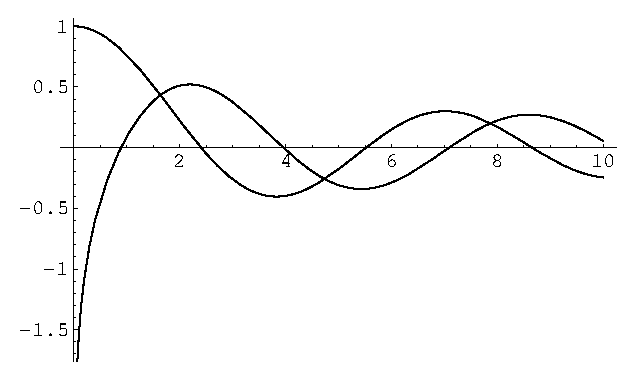
\includegraphics[width=10cm]{Bessel/BesselJY0.eps}
\caption{$J_0$ と $Y_0$ のグラフ
(\texttt{Plot[\{BesselJ[0,x],BesselY[0,x]\},\{x,0,10\}]})}
\end{figure}

また、UNIX の数学関数ライブラリィに入っている \texttt{y0(x)}, 
\texttt{y1(x)},  \texttt{yn(n,x)} も Weber の Bessel 関数 $Y_n$ であるようだ。

ついでに Wolfram MathWorld によると、
\begin{quote}
 A Bessel function of the second kind $Y_n(x)$ (e.g, Gradshteyn and Ryzhik
 2000, p. 703, eqn. 6.649.1), sometimes also denoted $N_n(x)$ (e.g,
 Gradshteyn and Ryzhik 2000, p. 657, eqn. 6.518), is a solution to the
 Bessel differential equation which is singular at the origin. Bessel
 functions of the second kind are also called Neumann functions or Weber
 functions.
\end{quote}
とある。

私なりの結論は、名前だけで議論するのは危険だ、
式で記号を定義・約束してから議論を始めるべきだ、
というものである。  \qed
\end{jremark}

\begin{screen}
\begin{jlemma}[Neumann 関数の性質]
  $t\ne 0$ に対して
\[
  Y_m(t)
  =\frac{1}{\pi}
    \left.
    \left(
            \frac{\rd J_\nu}{\rd \nu}(t)
     -(-1)^m\frac{\rd J_{-\nu}}{\rd \nu}(t)
    \right)
    \right|_{\nu=m},
\]
\[
  Y_m'(t)=\lim_{\nu\to m}Y_\nu'(t),
  \quad
  Y_m''(t)=\lim_{\nu\to m}Y_\nu''(t).
\]
\end{jlemma}
\end{screen}

  $\nu$を与えられた複素数として、$x=x(t)$ に関する微分方程式
\[
  x''(t)+\frac{1}{t}x'(t)+\left(1-\frac{\nu^2}{t^2}\right)x(t)=0
\]
を $\nu$ 次の \textbf{Bessel の微分方程式}という。

微分方程式だけを考える場合は、
$\mathrm{Re}\;\nu\ge 0$ として一般性を失わない
($\mathrm{Re}\;\nu<0$ のときは、$-\nu$ を$\nu$ と置き直せばよい)。
しかし $\mathrm{Re}\;\nu<0$ に対しても $J_\nu(z)$ を考えたいので、
それはしない。

Bessel の微分方程式は、
$t=0$ を確定特異点に持つ\footnote{微分方程式 $x^{(n)}(t)
+a_1(t)x^{(n-1)}(t)+\cdots+a_{n-1}(t)x'(t)+a_n(t)x(t)=0$ が $t=0$ を
確定特異点に持つとは、
$t^k a_k(t)$ ($1\le k\le n$) が $t=0$ の近傍で正則なことをいう。
内輪向けのノートだが、「常微分方程式ノート」
(桂田 \cite{桂田常微分ノート}) に、確定特異点の話を書いておいた。}。

\begin{screen}
\begin{jtheorem}[Besselの微分方程式の一般解]
\label{jtheorem:ベッセルの微分方程式の一般解}
  $\nu\in\C$ とする。
\begin{enumerate}[(1)]
\item
  $\nu\not\in\Z$ のとき
\[
  x(t)=c_1 J_{\nu}(t)+c_2 J_{-\nu}(t)\quad\mbox{($c_1$, $c_2$ は任意定数)}
\]
は $\nu$ 次 Bessel の微分方程式の一般解である。
\item
  $\nu$ が何であっても
\[
  x(t)=c_1 J_{\nu}(t)+c_2 Y_{\nu}(t)\quad\mbox{($c_1$, $c_2$ は任意定数)}
\]
は $\nu$ 次 Bessel の微分方程式の一般解である。
\end{enumerate}
\end{jtheorem}
\end{screen}
\begin{proof}
  ロンスキアン $W(f,g):=\det\left(\begin{array}{cc}f & g \\ f' &g'
\end{array}\right)$ を調べると、
\[
  W(J_\nu(z),J_{-\nu}(z)) =-\frac{2\sin\nu\pi}{z},\quad
  W(J_\nu(z),Y_{\nu}(z)) =\frac{2}{\pi z}
\]
となるので、$\nu\not\in\N_0$ であれば $W(J_\nu(z),J_{-\nu}(z))\ne 0$,
また $\nu$ が何であっても $W(J_\nu(z),Y_{\nu}(z))\ne 0$. \qed
\end{proof}

$m\in\Z$ のとき $J_{-m}(t)=(-1)^m J_{m}(t)$ が成り立つので、
$\nu=m\in\Z$ の場合は $x(t)=c_1 J_{\nu}(t)
+c_2 J_{-\nu}(t)$ は一般解とならないことが明らかである
(もちろんロンスキアンからも分かる)。
なお、非整数の $\nu$ に対しては、
$J_\nu$, $J_{-\nu}$ の間にこのような比例関係はない。
例えば
\begin{equation}
  J_{1/2}(x)=\left(\frac{2}{\pi x}\right)^{1/2}\sin x,\quad
  J_{-1/2}(x)=\left(\frac{2}{\pi x}\right)^{1/2}\cos x,
  \label{eq:1/2のBessel関数1}
\end{equation}
\begin{equation}
  J_{3/2}(x)=\left(\frac{2}{\pi x}\right)^{1/2}
  \left(\frac{\sin x}{x}-\cos x\right),\quad
  J_{-3/2}(x)=\left(\frac{2}{\pi x}\right)^{1/2}
  \left(-\sin x-\frac{\cos x}{x}\right)
  \label{eq:1/2のBessel関数2}
\end{equation}
であることに注目しよう
($J_\nu$ を定義する級数を整理すれば容易に求まる)。

\begin{screen}
\begin{jcorollary}
  $\nu\in\C$, $k\ne 0$ とする。微分方程式
\begin{equation}
  x''(t)+\frac{1}{t}x'(t)+\left(k^2-\frac{\nu^2}{t^2}\right)x(t)=0
  \label{eq:kの入ったベッセルの微分方程式}
\end{equation}
について、以下の (1), (2) が成り立つ。
\begin{enumerate}[(1)]
\item
  $\nu\not\in\Z$ のとき
\[
  x(t)=c_1 J_{\nu}(k t)+c_2 J_{-\nu}(k t)\quad\mbox{($c_1$, $c_2$ は任意定数)}
\]
は微分方程式 (\ref{eq:kの入ったベッセルの微分方程式}) の一般解である。
\item
  $\nu$ が何であっても
\[
  x(t)=c_1 J_{\nu}(k t)+c_2 Y_{\nu}(k t)\quad\mbox{($c_1$, $c_2$ は任意定数)}
\]
は微分方程式 (\ref{eq:kの入ったベッセルの微分方程式}) の一般解である。
\end{enumerate}
\end{jcorollary}
\end{screen}

\subsection{寝た子を起こす話}

\subsubsection{問題のありか}
  前項であげた定義式
\begin{equation}
  J_\nu(z)=\left(\frac{z}{2}\right)^\nu\sum_{m=0}^\infty
 \frac{(-1)^m}{m!\itGamma(m+\nu+1)}\left(\frac{z}{2}\right)^{2m}
  \label{eq:もう一度定義式}
\end{equation}
について、説明を補足する。一言で言うと、
$\nu$ が整数で無い場合、
$(z/2)^\nu$ は $0$ で特異性を持つことに注意する必要がある、
ということだが、
細かい話ではあるし、
$\nu\in\Z$ の場合しか考えないときには一切必要がないので
(せいぜい \ref{subsubsec:次数が整数の場合} を見れば十分)、
急いでいるときは飛ばしても構わない。

\subsubsection{簡単な $\nu\in\Z$ の場合を片付けておく}
\label{subsubsec:次数が整数の場合}

$\nu=n\in\Z$ のとき、後で証明するように
\[
 m\in\N\quad\Then\quad J_{-m}(z)=(-1)^m J_m(z)
\]
が成り立つので、$n\ge 0$ を考えてから裏返すということをやればよい。
$J_n(z)$ 自身が整関数になり、$m:=|n|$ とおくとき
\[
  J_n(z)\sim \frac{z^m}{2^m m!}\quad\mbox{($z\to 0$)}
\]
が成り立つ。特に
\[
  J_n(0)=\left\{
  \begin{matrix}
   1 & \mbox{($n=0$)} \\
   0 & \mbox{($n\ne0$)}.
  \end{matrix}
  \right.
\]

\subsubsection{$\nu\not\in\Z$ の場合 (問題点をウォッチ)}

  式 (\ref{eq:もう一度定義式}) の $\sum$ の部分
\[
  e_\nu(z):=\sum_{m=0}^\infty
 \frac{(-1)^m}{m!\itGamma(m+\nu+1)}\left(\frac{z}{2}\right)^{2m}
\]
は容易に整関数であることが証明でき (例えば d'Alembert の収束判定法)、
\[
  e_{\nu}(0)=\frac{1}{\itGamma(\nu+1)}\ne 0
\]
ということも分かる。
従って $J_\nu$ は $z\mapsto (z/2)^\nu$ と同じ特異性を持つことが分かる。

以下、この文書では $\nu\in\R$ の場合のみを考えることにする。
この文書の目的には明らかにそれで十分であるので、
$\nu$ が虚数である場合の議論をさぼっても構わないであろう。

\subsubsection{$\nu\in\R\setminus\Z$ の場合 --- 方針}

高等学校で、$a>0$ に対して、指数関数 $\R\ni x\mapsto a^x\in\R$ を学んだ。
従って、
$z>0$, $\nu\in\R$ に対しては、
冪乗 $z^\nu$ は定義済みであると言える。
正数でない $z$ に対して $z^\nu$ をいかに定めるかが問題であるが、
大ざっぱに言って、
\[
  z^\nu=\exp\left(\nu\log z\right)
\]
という等式を基礎にする。この右辺に現れる $\log z$ が曲者である。

\subsubsection{寄り道?: 多価関数としての $z^\nu$}

複素関数論で、多価関数としての $\log z$ について学んだはずである。
与えられた $z$ に対して $\exp w=z$ を満たす $w$ を $z$ の対数と呼んで、
$\log z$ と表すのであるが、
$w$ が一意的には定まらないのが注意を要するところである。

\begin{screen}
\begin{jlemma}
  $z=r e^{i\theta}$ ($r>0$, $\theta\in\R$) とするとき、
任意の $w\in\C$ に対して、次が成り立つ。
\[
 \exp w=z
 \quad\LongIff\quad
 \exists k\in\Z\quad\mbox{s.t.}\quad w=\log|z|+ i(\theta+2 k\pi).
\]
ただし、右辺に現れる $\log|z|$ は $e^y=|z|$ を満たす $y\in\R$ (これは
一意的に存在する) を意味する。
\end{jlemma}
\end{screen}
\begin{proof}
  (流石に簡単なので省略する。) \qed
\end{proof}

要するに、ここで定義した「関数」 $\log z$ は無限多価である
(通常の意味の写像にはならない)。
そのため、
\begin{align*}
 z^\nu=\exp(\nu\log z)
  =\exp\left\{\nu\left[\log|z|+i(\theta+2k\pi)\right]\right\}
  =|z|^\nu e^{i\nu\theta}\exp\left(2i\nu k\pi\right)\\
 \mbox{($|z|^\nu$ は高校数学の意味での巾乗)}
\end{align*}
も多価関数になりうる (最後の因子に注意)\footnote{ただし、
$\nu\in\Z$ のときは、
$\exp(2 i\nu k\pi)=1$ であるから、値が一つに定まる。}。
例えば $\nu=\dfrac{1}{\ell}$ ($\ell\in\Z$) の場合、
$z^\nu:=\exp(\nu\log z)$ は $|\ell|$ 価関数である。

しかし、$\left|z^\nu\right|=|z|^\nu$ は成立する。
ここで $\nu\in\R$ であることが効いていることに注意しよう。

\subsubsection{本道?: 主値}

  $z=r e^{i\theta}$ ($r>0$, $\theta\in(-\pi,\pi)$) に対して、
\[
  \Log z:=\log r+i\theta
\]
と定め、これを $z$ の対数の主値と呼ぶ。

  複素平面から負軸を除いた領域 $\Omega:=\C\setminus(-\infty,0]$ において、
写像 $\Log\colon\Omega\ni z\mapsto \Log z\in\C$ が定まるが、
これは正則関数となる。
これは高校数学の意味での対数関数の拡張になっていて、
\[
  \frac{\D}{\D z}\Log z=\frac{1}{z},\quad
  \exp\left(\Log z\right)=z
\]
を満たす。

  我々は $\nu\in\R$, $z\in\Omega=\C\setminus(-\infty,0]$ に対して、
\[
  z^\nu:=\exp\left(\nu\Log z\right)
\]
として $z^\nu$ を定める。
\[
  \forall z\in\Omega\quad
  \left(z^\nu\right)'=\nu z^{\nu-1},\quad
  \left|z^\nu\right|=|z|^\nu\quad\mbox{($|z|^\nu$ は高校数学の巾乗)}
\]
が成り立つ。特に
\[
 \lim_{z\in\Omega\atop z\to0}z^\nu=
 \left\{
  \begin{matrix}
   0 & \mbox{($\nu>0$)}\\
   \infty & \mbox{($\nu<0$)}.
  \end{matrix}
 \right.
\]
これから $\nu>0$ の場合、$0^\nu=0$ と約束すると、
$J_\nu(z)$ は $\Omega\cup\{0\}$ 上の連続関数に拡張できることが分かる。

\begin{yodan}[もしも $\nu\in\R$ でなければ]
  やはり対数の主値 $\Log$ を用いて
\[
  z^\nu:=\exp\left(\nu\Log z\right)
\]
により $z^\nu$ を定める。こうしても
\[
 \frac{\D}{\D z}z^\nu=\nu z^{\nu-1}
\]
は成り立つ。しかし $\left|z^\nu\right|$ はあまり簡単ではない。

  $\nu=\alpha+i\beta$ ($\alpha$, $\beta\in\R$) とするとき、
$z=re^{i\theta}$ ($r>0$, $\theta\in(-\pi,\pi)$) に対して、
\begin{align*}
  z^\nu&=\exp\left(\nu\Log z\right)
       =\exp\left[(\alpha+i\beta)\left(\log r+i\theta\right)\right]\\
       &=\exp
        \left[
          (\alpha\log r-\beta\cdot\theta)
          +i\left(\beta\log r+\alpha\cdot\theta\right)
        \right]
\end{align*}
であるから
\[
  \left|z^\nu\right|
  =\exp
        \left(\alpha\log r-\beta\cdot\theta\right)
  =r^\alpha e^{-\beta\cdot\theta}\le r^\alpha e^{|\beta|\pi}.
\]
  特に $\alpha=\MyRe\nu>0$ である場合は
\[
  \lim_{z\to 0\atop z\in\Omega} z^\nu=0.
\]
  主値でない場合は $|z^\nu|$ 自体が無限多価であり、
$\dsp\lim_{z\to 0\atop z\in\Omega} z^\nu=0$ も成立しないが、
主値を選ぶということで何とかなりそうである。 \qed
\end{yodan}

\section{$J_n(z)$ の基本的な性質}

  $n\in\N_0$ に対する Bessel 関数の性質を列挙する。

\begin{enumerate}
\item
  任意次数の Bessel 関数の零点はすべて実数であり、
$0$ を中心として対称に分布する。
\item
  任意次数の Bessel 関数の零点は単純である。
\item
\[
  \frac{\D}{\D z}\left(z^{-n}J_n(z)\right)=-z^{-n}J_{n+1}(z),\quad
  \frac{\D}{\D z}\left(z^{n+1}J_{n+1}(z)\right)=z^{n+1}J_{n}(z).
\]
\item
  $J_n$ と $J_{n+1}$ の零点は重なることなく、
交互に並んでいる。
\item
  任意の$m\in\N$に対して、$J_n$ と $J_{n+m}$ は共通零点を持たない。
\item
  $n$ 次 Bessel 関数 $J_n(t)$ の正の零点は無限個存在するが、
小さい方から順に並べたものを $\{\mu_{n m}\}_{m\in\N}$ とすると、
\[
  \lim_{m\to\infty} \mu_{n m}=\infty,
\]
もっと詳しく
\[
  \lim_{m\to\infty} (\mu_{n,m+1}-\mu_{n,m})=\pi
\]
が成り立つ (つまり、$J_n(t)$ は $t$ が大きいところでは、零点の間隔がほ
ぼ $\pi$ に等しい、ということである)。さらに
\[
  \lim_{n\to\infty} (\mu_{n+1,1}-\mu_{n,1})=1.
\]
\item
  $0<x\ll1$ に対して (というよりも $x\to 0$ のときと言うべき?)
\begin{align*}
  J_n(x)&\sim \frac{1}{2^n n!}x^n\quad\mbox{($n=0,1,\dots$)},\\[1em]
 Y_n(x)&\sim
 \left\{
 \begin{array}{ll}
  \dfrac{2}{\pi}\log x          & \mbox{($n=0$)} \\
  -\dfrac{2^n(n-1)!}{\pi}x^{-n} & \mbox{($n\in\N$)}.
 \end{array}
 \right.
\end{align*}
%
  $x\gg n$ のとき (というよりも $x\to\infty$ のときと言うべき?)
\[
  J_n(x)\sim\sqrt{\frac{2}{\pi x}}\cos\left(x-(2n+1)\frac{\pi}{4}\right),
\]
\[
  Y_n(x)\sim\sqrt{\frac{2}{\pi x}}\sin\left(x-(2n+1)\frac{\pi}{4}\right).
\]
%
\item
  (整数次 Bessel 関数の母関数)
\[
  \exp\left[\frac{x}{2}\left(t-\frac{1}{t}\right)\right]
  =\sum_{n=-\infty}^{\infty}J_n(x)t^n.
\]
\end{enumerate}

\subsection{零点に関する性質とその証明}

  $\nu\in\R$ とするとき、$J_\nu$ の零点について調べる。

  ものすごく大ざっぱには、$J_\nu$ は Bessel の微分方程式
\[
  w''(z)+\frac{1}{z}w'(z)+\left(1-\frac{\nu^2}{z^2}\right)w(z)=0
\]
の解であり、この方程式は $|z|$ が大きいとき、単振動の方程式
\[
  w''(z)+w(z)=0\quad\mbox{(この解は三角関数 $w(z)=A\cos z+B\sin z$)}
\]
に「近い」から、Bessel 関数 $J_\nu(z)$は $z$ が大きいとき、
挙動が三角関数のそれに似ていると想像できる。

  まず、$J_\nu$ の零点は、$0$ であるか、
\[
  e_\nu(z):=\sum_{m=0}^\infty\frac{(-1)^m}{m!\itGamma(m+\nu+1)}
 \left(\frac{z}{2}\right)^{2m}
 \qquad\mbox{(この記号を以下しばらくの間だけ用いる)}
\]
の零点であるかのどちらかである。

\begin{screen}
\begin{jproposition}
  $\nu\in\R$ とするとき、$J_\nu$ は ($0$ 以外の) 純虚数の零点は持たない。
\end{jproposition}
\end{screen}
\begin{proof}
これには $e_\nu$ が ($0$ 以外の) 純虚数の零点は持たないことを確かめればよい。

$z=i t$ ($t\in\R$, $t\ne 0$) とするとき、
\[
 e_\nu(it)=\sum_{m=0}^\infty\frac{(-1)^m}{m!\itGamma(m+\nu+1)}\frac{(-1)^m
 t^{2m}}{2^{2m}}
 =\sum_{m=0}^\infty\frac{1}{m!\itGamma(m+\nu+1)}\left(\frac{t^2}{4}\right)^{m}.
\]
  これは $0$ 以上の項の和であり、十分大きい $m$ に対して、
第 $m$ 項は正であるから、$e_\nu(it)>0$.
ゆえに $e_\nu$ は純虚数の零点は持たない。 \qed
\end{proof}

\begin{screen}
\begin{jlemma}
  $\nu\in\R$ とするとき、
\[
 z\in\C\setminus(-\infty,0]\quad\Then\quad
 \overline{J_\nu(z)}=J_\nu(\overline z).
\]
\end{jlemma}
\end{screen}
\begin{proof}
$e_\nu(z)$ を定義する級数の係数は実数であるから、
\[
 \overline{e_\nu(z)}=e_\nu(\overline z)\quad\mbox{($z\in\C$)}
\]
が成り立つ。

一方、
\[
  \nu\in\R,\quad z\in\C\setminus(-\infty,0]\quad\Then\quad
  \overline{z^\nu}=\left(\overline z\right)^\nu
\]
が成り立つ\footnote{実際、$z=re^{i\theta}$ ($r>0$, $\theta\in(-\pi,\pi)$) とするとき、
\[
  z^\nu=\exp\left(\nu\Log z\right)=\exp\left[\nu(\log r+i\cdot\theta)\right]
  =r^\nu\exp(i\nu\theta)
\]
であり、一方 $\overline z=r e^{-i\theta}$ であるから
\[
 \left(\overline z\right)^\nu=\exp\left(\nu\Log\overline z\right)
    =\exp\left[\nu(\log r-i\theta)\right]
  =r^\nu\exp(-i\nu\theta)
  =\overline{r^\nu\exp(i\nu\theta)}
  =\overline{z^\nu}.
\]}。
ゆえに
\[
 \overline{J_\nu(z)}
 =\overline{\left(\frac{z}{2}\right)^\nu e_{\nu}(z)}
 =\overline{\left(\frac{z}{2}\right)^\nu}\overline{e_{\nu}(z)}
 =\left(\frac{\overline z}{2}\right)^\nu e_{\nu}(\overline z)
 =J_\nu(\overline z). \qed
\]
\end{proof}
\begin{screen}
\begin{jproposition}
  $\nu\in\R$ とするとき、$J_\nu$ は虚数の零点を持たない。
\end{jproposition}
\end{screen}
\begin{proof}
  $J_\nu$ が虚数の零点 $\mu=\alpha+i\beta$ ($\alpha$, $\beta\in\R$,
$\beta\ne0$) を持つと仮定する。このとき補題によって、
$\overline\mu=\alpha-i\beta$ も零点になる。
\begin{align*}
 \int_0^1 x\left|J_\nu(\mu x)\right|^2\Dx
 &=\int_0^1 xJ_\nu(\mu x)\overline{J_\nu(\mu x)}\;\Dx
  =\int_0^1 xJ_\nu(\mu x){J_\nu(\overline\mu x)}\;\Dx\\
 &=\frac{1}{\mu^2-\overline\mu^2}
   \left[
    \overline\mu J_\nu(\mu)J_\nu'(\overline\mu)
 -
    \mu J_\nu(\overline\mu)J_\nu'(\mu)
   \right]
  =0.
\end{align*}
  これから $J_\nu(\mu x)\equiv 0$ となるが、明らかな矛盾である。
--- 以上の議論は $\nu$ が小さいときは成立しない。
その場合の証明は準備中。 \qed
\end{proof}

\begin{screen}
\begin{jproposition}
  $\nu\in\R$ とする。
$J_\nu$ の正の零点全体は小さい方から順に番号づけることができる。
すなわち、狭義単調増加数列
\[
  0<\mu_{\nu,1}<\mu_{\nu,2}<\cdots
\]
が存在して、
$\{\mu_{\nu,m}\}\cup\{-\mu_{\nu,m}\}\cup\{0\}$ が $J_\nu$ の零点全体となる。
\end{jproposition}
\end{screen}
\begin{proof}
   上の命題から、$J_\nu$ の零点は実軸上にしか存在しない。
$J_\nu$ の零点は $0$ または $e_\nu$ の零点であり、
$e_\nu$ は偶関数または奇関数であるから、
$J_\nu$ の零点は $0$ に関して左右対称の位置にある。
また $e_\nu$ は恒等的に $0$ ではない整関数であるから、
零点は集積せず (「一致の定理」による)、
任意の有界な区間 $I\subset \R$ には有限個の零点しか存在しないことが分かる。 \qed
\end{proof}

この時点ではまだ零点が無限個存在することを証明していない。

次の補題は、ボウマン \cite{ボウマン} を参考にした。
\begin{screen}
\begin{jlemma}
  $\forall \nu\in\R$, $\forall k>1$, $\exists A>0$, $\forall a\ge A$,
$\exists x\in[a,a+\pi]$ s.t. $J_\nu(kx)=0$.
\end{jlemma}
\end{screen}
\begin{proof}
  $u(x):=\sqrt{k x}J_\nu(k x)$ とおくと、
$J_\nu(t)=t^{-1/2}u(t/k)$ となるので、
\begin{align*}
  &J_\nu'(t)=-\frac{1}{2}t^{-3/2}u\left(\frac{t}{k}\right)
            +t^{-1/2}u'\left(\frac{t}{k}\right),\\
  &J_\nu''(t)=\frac{3}{4}t^{-5/2}u\left(\frac{t}{k}\right)
            -\frac{1}{k}t^{-3/2}u'\left(\frac{t}{k}\right)+
             \frac{1}{k^2}t^{-1/2}u''\left(\frac{t}{k}\right).
\end{align*}
  Bessel の微分方程式に代入して整理すると
\[
  u''\left(\frac{t}{k}\right)
 +k^2\left[1+\left(\frac{1}{4}-\nu^2\right)t^{-2}\right]
  u\left(\frac{t}{k}\right)=0.
\]
  ゆえに
\begin{equation}
  u''(x)=-w(x)u(x),\quad
  w(x):=k^2-\left(\nu^2-\frac{1}{4}\right)x^{-2}.
  \label{eq:uについての微分方程式}
\end{equation}
  $v(x):=\sin(x-a)$ とおくと $v''=-v$ が成り立つ。
これに $u$ をかけた方程式から、
(\ref{eq:uについての微分方程式}) に $v$ を書けた方程式を辺々引き算すると
\[
 u(x)v''(x)-u''(x)v(x)=(w(x)-1)u(x)v(x).
\]
左辺が $\left[u(x)v'(x)-u'(x)v(x)\right]'$ に等しいことに注意して、
区間 $[a,a+\pi]$ で積分すると
\[
 \left[u(x)v'(x)-u'(x)v(x)\right]_{a}^{a+\pi}
  =\int_a^{a+\pi}(w(x)-1)u(x)v(x)\;\Dx.
\]
左辺については、$v(a)=v(a+\pi)=0$, $v'(a)=1$, $v'(a+\pi)=-1$ であるから
\[
 \left[u(x)v'(x)-u'(x)v(x)\right]_{a}^{a+\pi}=-u(a+\pi)-u(a).
\]
一方、右辺については、
$a$ を十分大きく取ると $[a,\infty)$ で $w(x)-1>0$ であり、
また一般に $(a,a+\pi)$ で $v>0$ であるから、
$(a,a+\pi)$ で $(w(x)-1)v(x)>0$.
また $a>0$ ならば $[a,\infty)$ で $u$ は連続であるので、
積分の平均値の定理から、
\[
 \exists\xi\in[a,a+\pi]\quad\mbox{s.t.}\quad
 \int_a^{a+\pi}(w(x)-1)u(x)v(x)\;\Dx=u(\xi)\int_a^{a+\pi}(w(x)-1)v(x)\;\Dx.
\]
ゆえに
\[
 -(u(a+\pi)+u(a))=u(\xi)\int_a^{a+\pi}(w(x)-1)v(x)\;\Dx.
\]
  右辺の積分は正であるから、$u(a)$, $u(a+\pi)$, $u(\xi)$ の3つが
すべて正になったり、あるいはすべて負になったりすることはあり得ない。
ゆえに少なくとも一つが $0$ になるか、正のものと負のものが存在する。
後者の場合は中間値の定理を用いて、
結局 $u$ は $[a,a+\pi]$ のどこかで $0$ になることが分かる。 \qed
\end{proof}

\begin{screen}
\begin{jproposition}
  $\nu\in\R$ とするとき、$J_\nu$ の正の零点は無限個存在し、
小さい方から順に並べたものを $\{\mu_{\nu,m};m\in\N\}$ とするとき、
\[
  \lim_{m\to\infty}\mu_{\nu,m}=\infty.
\]
\end{jproposition}
\end{screen}
\begin{proof}
  零点が無限個存在することは補題から分かる。集積点を持たないので、
$\infty$ に発散する。 \qed
\end{proof}

\begin{screen}
\begin{jproposition}[$J_\nu$ の $0$ でない零点は単純である]
  $\nu\in\R$ とするとき、$\mu\ne 0$ が $J_\nu$ の零点ならば
  $J_\nu'(\mu)\ne 0$.
\end{jproposition}
\end{screen}
\begin{proof}
  $J_\nu(\mu)=0$ であるから、$\mu\in\R$ であることに注意する。
$J_\nu'(\mu)=0$ とすると、
$t=\mu$ を初期時刻とする常微分方程式の初期値問題
\[
  u''(t)+\frac{1}{t}u'(t)+\left(1-\frac{\nu^2}{t^2}\right)u(t)=0,\quad
  u(\mu)=u'(\mu)=0
\]
の解は、
解の一意性により $u(t)\equiv 0$ でなければならない。
ゆえに $J_\nu(t)\equiv 0$. これは矛盾であるから $J_\nu'(\mu)\ne 0$. \qed
\end{proof}
\begin{proof}
  $w=J_\nu(z)$ は Bessel の微分方程式
\[
  w''+\frac{1}{z}w'+\left(1-\frac{\nu^2}{z^2}\right)w=0
\]
の解である。$\mu\ne 0$ が $J_\nu(\mu)=J_\nu'(\mu)=0$ を満たすならば、
微分方程式に代入して、
\[
  J_\nu''(\mu)=0
\]
が成り立つ。微分方程式を $z$ で微分してから $z=\mu$ を代入するという操作
を続けていくと
\[
  J_\nu^{(m)}(\mu)=0\quad\mbox{($m=0,1,2,\cdots$)}
\]
が得られる。これから $J_\nu(z)\equiv 0$ が得られ、矛盾となる。 \qed
\end{proof}

\begin{screen}
\begin{jlemma}
\[
  \frac{\D}{\D
  z}\left(z^{-\nu}J_\nu(z)\right)=-z^{\nu}J_{\nu+1}(z),\quad
  \frac{\D}{\D z}\left(z^{\nu+1}J_{\nu+1}(z)\right)=z^{\nu+1}J_{\nu}(z).
\]
\end{jlemma}
\end{screen}
\begin{proof}
  単なる計算である。 \qed
\end{proof}
\begin{screen}
\begin{jproposition}
  $J_\nu$ の零点と $J_{\nu+1}$ の零点は互い違いに並んでいる。
\end{jproposition}
\end{screen}
\begin{proof}
  $\alpha$ と $\beta$ ($0<\alpha<\beta$) が $J_\nu$ の零点であるとするとき、
これらは $f(t):=t^{-\nu}J_\nu(t)$ の零点でもある。
Rolle の定理から、
\[
  \exists \gamma\in(\alpha,\beta)\quad\mbox{s.t.}\quad f'(\gamma)=0.
\]
$f'(t)=-t^{-\nu}J_{\nu+1}(t)$ であるから、
$-\gamma^{-\nu}J_{\nu+1}(\gamma)=0$. ゆえに $J_{\nu+1}(\gamma)=0$.
ゆえに「$J_\nu$ の二つの正の零点の間には $J_{\nu+1}$ の零点が存在する」。

同様にして「$a$ と $b$ ($0\le a<b$) が $J_{\nu+1}$ の零点であるとするとき、
$J_\nu(c)=0$ を満たす $c\in(a,b)$ が存在する」。
\qed
\end{proof}

\begin{screen}
\begin{jproposition}[零点の分布]
  $\nu\in\R$ とするとき、
$J_\nu$ の正の零点を小さい方から順に並べたものを $\{\mu_{\nu,m};
m\in\N\}$ とするとき、
\[
 \lim_{m\to\infty}\left(\mu_{\nu,m+1}-\mu_{\nu,m}\right)=\pi.
\]
 ($J_\nu(t)$ は $t$ が大きいところでは、零点の間隔はほぼ $\pi$ に
等しい --- 三角関数に近いと言ったことの裏付け。)
さらに
\[
  \lim_{\nu\to\infty}\left(\mu_{\nu+1,1}-\mu_{\nu,1}\right)=1.
\]
\end{jproposition}
\end{screen}
\begin{proof}
  前半は例えば大谷 \cite{大谷常微分} に書いてある (定理 6.5)。 \qed
\end{proof}

\begin{screen}
\begin{jproposition}
  任意の $\nu\in\R$ と任意の $m\in\N$ に対して、
$J_\nu$ と $J_{\nu+m}$ は共通の零点を持たない。
\end{jproposition}
\end{screen}
\begin{proof}
  (これは金子 \cite{金子} に書いてあった命題。準備中…)
\[
  J_{\nu+m}(z)=R_{\nu,m}(z)J_{\nu+1}(z)+S_{\nu,m}(z)J_{\nu}(z)
\]
と書けることと、Siegel の定理「$s$ が $0$ でない代数的数のとき、
$J_\nu(s)$ は超越数である。」による。\qed
\end{proof}

\section{Fourier-Bessel 展開}

  $u(x):=J_\nu(\alpha x)$,   $v(x):=J_\nu(\beta x)$ とおくと、
\begin{align}
  &x u''+u'+\left(\alpha^2-\frac{\nu^2}{x^2}\right)x u=0,
  \label{eq:uの微分方程式}\\
  &x v''+v'+\left(\beta^2-\frac{\nu^2}{x^2}\right)x v=0
\end{align}
であるから、第1式に $v$ をかけたものから、
第2式に $u$ をかけたものを引くと
\[
  x(u''v-v''u)+(u'v-v'u)+(\alpha^2-\beta^2)x u v=0.
\]
これから
\[
 \frac{\D}{\D x}\left[x (u'v-u v')\right]
 =\left(\beta^2-\alpha^2\right)x u v
\]
が得られる。

$\nu\in\N_0$ として\footnote{もっと緩い条件で良いように
書いてある本もあったが、筆者は納得できなかった。
$x u v$ が $[0,1]$ で可積分であるだけでなく、
$x\to 0$ のとき $x(u'v-uv')\to 0$ となる必要がある。
$\MyRe\nu>0$ などの条件が必要ではないか?
この種の議論が省略されている本が多く、少々イライラさせられる。
こういうところは Bourbaki 流に明解に書いて欲しいものだ。}
両辺を $[0,1]$ で積分すると
\begin{equation}
 \left(\beta^2-\alpha^2\right)\int_0^1 x J_\nu(\alpha x)J_\nu(\beta x)\;\Dx
 =\alpha J_\nu'(\alpha)J_\nu(\beta)-\beta J_\nu'(\beta)J_\nu(\alpha).
  \label{eq:Lommel}
\end{equation}
これを \textbf{Lommel の積分}という。

  式 (\ref{eq:uの微分方程式}) の両辺に $x u'(x)$ をかけて
\[
  2x^2 u'' u'+2x\left(u'\right)^2+2(\alpha^2 x^2-\nu^2) u u'=0.
\]
  これから
\begin{align*}
 \frac{\D}{\Dx}
 \left[
  x^2\left(u'\right)^2+(\alpha^2 x^2-\nu^2)u^2
 \right]
 &=2x\left(u'\right)^2
   +x^2\cdot 2u''u'+2\alpha^2 x u^2
   +2(\alpha^2x^2-\nu^2)u u' \\
 &=2\alpha^2x u^2.
\end{align*}
  $u=J_\nu(\alpha x)$, $u'=\alpha J_\nu'(\alpha x)$ を代入すると
\[
  \frac{\D}{\D x}
 \left[
  \alpha^2x^2J_\nu'(\alpha x)^2
 +(\alpha^2 x^2-\nu^2)J_\nu(\alpha x)^2
 \right]
 =2\alpha^2 x J_\nu(\alpha x)^2.
\]
この左辺を、Bessel 関数の漸化式から得られる
\begin{align*}
  J_\nu(t)^2-J_{\nu-1}(t)J_{\nu+1}(t)
  &=J_\nu(t)^2
   -\left(\frac{\nu}{t}J_{\nu}(t)+J_{\nu}'(t)\right)
    \left(\frac{\nu}{t}J_{\nu}(t)-J_{\nu}'(t)\right)\\
  &=J_\nu(t)^2-\left(\frac{\nu^2}{t^2}J_\nu(t)^2-J_\nu'(t)^2\right)
  =J_\nu'(t)^2+\left(1-\frac{\nu^2}{t^2}\right)J_\nu(t)^2
\end{align*}
を用いて変形すると
\[
 \frac{\D}{\D x}
  \left[
    x^2\left(J_\nu(\alpha x)^2-J_{\nu-1}(\alpha x)J_{\nu+1}(\alpha
    x)\right)
  \right]
  =
  2xJ_\nu(\alpha x)^2.
\]
これを $[0,1]$ で積分すると
\[
 2\int_0^1 x J_\nu(\alpha x)^2\;\D x
 =\left[
   x^2\left(J_\nu(\alpha x)^2-J_{\nu+1}(\alpha x)J_{\nu-1}(\alpha x)\right)
  \right]_0^1
 =J_\nu(\alpha)^2-J_{\nu+1}(\alpha)J_{\nu-1}(\alpha).
\]
すなわち
\begin{equation}
 \int_0^1 x J_\nu(\alpha x)^2\;\D x
 =\frac{1}{2}\left(J_\nu(\alpha)^2-J_{\nu+1}(\alpha)J_{\nu-1}(\alpha)\right).
 \label{eq:Lommel2}
\end{equation}

  $\alpha$ と $\beta$ を Bessel 関数の零点に選ぶと直交性が得られる。
\begin{screen}
\begin{jproposition}[Bessel 関数の直交関係式]
  $\nu\in\N_0$ とするとき、
$J_\nu$ の正の零点を小さい方から順に
\[
  \mu_{\nu,1}<\mu_{\nu,2}<\cdots
\]
とおくと、
\[
 \int_0^1 r J_\nu(\mu_{\nu,n}r)
          J_\nu(\mu_{\nu,m}r)\D r
  =\frac{J_{\nu+1}(\mu_{\nu,n})^2}{2}\delta_{nm}
 \quad\mbox{($n,m\in\N$)}
\]
\end{jproposition}
\end{screen}
(もしかすると $\MyRe\nu>0$ となる $\nu\in\C$ に対しても成立するのか?)
\begin{proof}
  まず (\ref{eq:Lommel}) に $J_\nu(\alpha)=J_\nu(\beta)=0$ を代入すると、
\[
  (\beta^2-\alpha^2)\int_0^1 x J_\nu(\alpha x)J_\nu(\beta x)\;\Dx=0.
\]
ここで $\alpha\ne\beta$ ならば、割り算により直交関係
\[
 \int_0^1 x J_\nu(\alpha x)J_\nu(\beta x)\;\Dx=0
\]
が得られる。

  一方、漸化式
\[
  \frac{2\nu}{t}J_{\nu}(t)=J_{\nu-1}(t)+J_{\nu+1}(t)
\]
の $t$ に、$J_\nu(\alpha)=0$ を満たす $\alpha\ne 0$ を代入すると
\[
  J_{\nu-1}(\alpha)=-J_{\nu+1}(\alpha)
\]
が得られるので、 (\ref{eq:Lommel2}) に代入して
\[
 \int_0^1 xJ_\nu(\alpha x)^2\;\Dx
 =\frac{1}{2}\left(0^2-J_{\nu+1}(\alpha)\left(-J_{\nu+1}(\alpha)\right)\right)
 =\frac{J_{\nu+1}(\alpha)^2}{2}.  \qed
\]
\end{proof}

\begin{screen}
\begin{jtheorem}[Bessel の展開]
  $f\colon (0,1)\to\C$ が連続で、
$\dsp\int_0^1\sqrt{x}f(x)\,\D x$ が絶対収束するとき、
$f$ が有界変分であるような任意の閉区間 $I\subset (0,1)$ の任意の $x$,
任意の $n\in\N\cup\{0\}$ に対して、
\[
  f(x)=\sum_{j=1}^\infty A_j J_n(\lambda_j x)
\]
が成り立つ。ただし
\[
  A_j:=\frac{2}{J_{n+1}(\lambda_j)^2}
  \int_0^1 x f(x)J_n(\lambda_j x)\;\D x
 \quad\mbox{($j\in\N$)}
\]
で、$\lambda_j$ は $J_n$ の正の零点を小さい順に並べたものである:
\[
 \{x>0; J_n(x)=0\}=\{\lambda_j\}_{j\in\N},\quad
 0<\lambda_1<\lambda_2<\cdots<\lambda_{j}<\lambda_{j+1}<\cdots.
\]
\end{jtheorem}
\end{screen}

  次のような展開も可能である。
\begin{enumerate}[(1)]
\item
\[
  f(x)=B_0 x^n+\sum_{j=1}^\infty B_j J_n(\mu_j x),
\]
\begin{align*}
  &B_0=(2n+2)\int_0^1 f(x)x^{n+1}\;\Dx,\\
  &B_j=\frac{2}{J_n(\mu_j)^2}\int_0^1 x f(x)J_n(\mu_j x)\;\Dx
 \quad\mbox{($j\in\N$)}.
\end{align*}
ここで $\mu_j$ は $J_{n+1}(x)$ の零点を小さい方から順に並べたものである。
%
\item
  (Dini の展開) $h>0$ を任意に固定する。
\[
  f(x)=\sum_{j=1}^\infty C_j J_n(\nu_j x).
\]
ただし
\[
  C_j=\frac{2\nu_j^2}{\left[\nu_j^2-h(2n-h)\right]J_n(\nu_j)^2}
  \int_0^1 xf(x)J_n(\nu_j x)\;\Dx.
\]
ここで$\nu_j$ は
\[
  x J_{n+1}(x)-h J_n(x)=0
\]
の正根を小さい方から順に並べたものとする。
\end{enumerate}

\begin{jremark}[不連続関数の展開]
  $f$ が連続でなくて、
単に $\sqrt{x}f(x)$ が $(0,c)$ 上 Lebesgue 可積分とするだけで、
結果の等式を
\[
  \frac{f(x+0)+f(x-0)}{2}
  =\sum_{j=1}^\infty A_j J_n(\lambda_j x)
\]
で置き換えたものが成立する。 --- 普通の Fourier 級数と同じだ。 \qed
\end{jremark}

\begin{screen}
\begin{jtheorem}[Fourier-Bessel の展開]
\label{jtheorem:フーリエ・ベッセルの展開}
  円盤 $\{(x,y);x^2+y^2<1\}$ の完全系
\[
 f(r\cos\theta,r\sin\theta)=
  \frac{1}{2}\sum_{j=1}^\infty A_{0j}J_0(\mu_{0j}r)
 +\sum_{n=1}^\infty\sum_{j=1}^\infty
  J_n(\mu_{nj}r)
  (A_{nj}\cos n\theta+B_{nj}\sin n\theta)
\]
\[
  A_{nj}=\frac{2}{\pi J_{n+1}(\mu_{nj})^2}
  \int_0^1\left(\int_0^{2\pi}f(r\cos\theta,r\sin\theta)
  J_n(\mu_{nj}r)\cos n\theta\,\D\theta\right)r\;\D r,
\]
\[
  B_{nj}=\frac{2}{\pi J_{n+1}(\mu_{nj})^2}
  \int_0^1\left(\int_0^{2\pi}f(r\cos\theta,r\sin\theta)
  J_n(\mu_{nj}r)\sin n\theta\,\D\theta\right)r\;\D r.
\]
\end{jtheorem}
\end{screen}
\begin{proof}
  $r\in(0,1)$ を固定して、$\theta\mapsto f(r,\theta)$ を考えると、
Fourier 級数展開
\[
  f(r\cos\theta,r\sin\theta)=\frac{a_0(r)}{2}
 +\sum_{n=1}^\infty (a_n(r)\cos n\theta+b_n(r)\sin n\theta),
\]
\[
  a_n(r):=\frac{1}{\pi}\int_0^{2\pi}
          f(r\cos\theta,r\sin\theta)\cos n\theta\,\D\theta,
  \quad
  b_n(r):=\frac{1}{\pi}\int_0^{2\pi}
          f(r\cos\theta,r\sin\theta)\sin n\theta\,\D\theta
\]
が得られる。
  $a_n(r)$, $b_n(r)$ は $(0,1)$ 上の関数だから、
Fourier-Bessel 展開ができる。
\[
 a_n(r)=\sum_{j=1}^\infty A_{nj}J_n(\mu_{nj}r),\quad
 A_{nj}:=\frac{2}{J_{n+1}(\mu_{nj})^2}\int_0^1 r a_n(r)J_n(\mu_{nj}r)\,\D r,
\]
\[
 b_n(r)=\sum_{j=1}^\infty B_{nj}J_n(\mu_{nj}r),\quad
 B_{nj}:=\frac{2}{J_{n+1}(\mu_{nj})^2}\int_0^1 r b_n(r)J_n(\mu_{nj}r)\,\D r.
\]
以上まとめると定理を得る。 \qed
\end{proof}

\begin{screen}
\begin{jcorollary}
  円盤 $\{(x,y);x^2+y^2<R^2\}$ の完全系
\[
 f(r\cos\theta,r\sin\theta)=
  \frac{1}{2}\sum_{j=1}^\infty A_{0j}J_0(\mu_{0j}r)
 +\sum_{n=1}^\infty\sum_{j=1}^\infty
  J_n(\mu_{nj}r)
  (A_{nj}\cos n\theta+B_{nj}\sin n\theta)
\]
\[
  A_{nj}=\frac{2}{\pi R^2 J_{n+1}(\mu_{nj} R)^2}
  \int_0^R\left(\int_0^{2\pi}f(r\cos\theta,r\sin\theta)
  J_n(\mu_{nj}r)\cos n\theta\,\D\theta\right)r\;\D r,
\]
\[
  B_{nj}=\frac{2}{\pi R^2 J_{n+1}(\mu_{nj} R)^2}
  \int_0^R\left(\int_0^{2\pi}f(r\cos\theta,r\sin\theta)
  J_n(\mu_{nj}r)\sin n\theta\,\D\theta\right)r\;\D r.
\]
\end{jcorollary}
\end{screen}

\section{Bessel の微分方程式を素朴に解いてみる}

  (要するに Bessel の微分方程式は未定係数法もどきで解くことができ、
自然に Bessel 関数が得られる、という話である。)

  Bessel の微分方程式は $t=0$ を確定特異点に持つので、
\textbf{Frobenius の理論}で扱うことができるが
(桂田 \cite{桂田常微分ノート})、
そういう ``一般論を知っていると仮定しての説明'' はやめて、
素朴に始めてみよう。
%
\[
 x(t)=\sum_{k=0}^\infty b_k t^{\lambda+k}\quad\mbox{($b_0\ne 0$)}
\]
%
の形に書けると仮定する\footnote{老婆心:
Bessel の微分方程式の係数は $t=0$ で正則ではないので、
$t=0$ で正則でない解がありうる。
こういう場合は (結果論になるが)、
普通のベキ級数ではなくて、$t^\lambda$ ($\lambda$ は
半端になりうる数) をかけた級数の形で解が得られる。}。微分方程式に代入して
%
\[
 \sum_{k=0}^\infty (k+\lambda)(k+\lambda-1)b_k x^{k+\lambda-2}
 +\sum_{k=0}^\infty (k+\lambda)b_kx^{k+\lambda-2}
 +\sum_{k=0}^\infty \left(1-\frac{n^2}{t^2}\right)b_k x^{k+\lambda}
 =0.
\]
整理すると
\[
 (\lambda^2-n^2)b_0 x^{\lambda-2}
 +\left[(\lambda+1)^2-n^2\right]b_1 x^{\lambda-1}
 +\sum_{k=0}^\infty
  \left([(k+\lambda+2)^2-n^2]b_{k+2}+b_k\right)x^{k+\lambda}=0.
\]
%
まず最低次の項の係数を考えて、
\[
 \lambda^2-n^2=0\quad\mbox{ゆえに}\quad \lambda=\pm n.
\]
%
\paragraph{$\lambda=n$ の場合}
  $x^{\lambda-1}$ の係数が $(n+1)^2-n^2\ne 0$ となるから $b_1=0$ で
なければならない。係数の漸化式は
%
\[
 b_{k+2}=-\frac{b_k}{(k+n+2)^2-n^2}=-\frac{b_k}{(k+2)(k+2n+2)}.
\]
%
これから
%
\begin{eqnarray*}
 b_2&=&-\frac{b_0}{2(2n+2)}=-\frac{n!b_0}{2^2(n+1)! 1!},\\
 b_4&=&-\frac{b_2}{4(2n+4)}= \frac{n!b_0}{2^4(n+2)! 2!},\\
 b_6&=&-\frac{b_4}{6(2n+6)}=-\frac{n!b_0}{2^6(n+3)! 3!},
\end{eqnarray*}
%
一般に
%
\[
 b_{2k}=\frac{(-1)^k n!}{2^{2k}(n+k)! k!} b_0,\quad
 b_{2k-1}=0 \quad\mbox{($k\in\N$)}
\]
%
したがって、このときの解は
%
\[
 x(t)=b_0 2^n n! \sum_{k=0}^\infty\frac{(-1)^k}{(n+k)!k!}
  \left(\frac{t}{2}\right)^{2k+n}.
\]
%
すなわち
\[
  x(t)=b_0 2^n n! J_n(t).
\]

\paragraph{$\lambda=-n$ の場合}
  漸化式が
%
\[
 b_{k+2}=-\frac{b_k}{(k-n+2)^2-n^2}=-\frac{b_k}{(k+2)(k-2n+2)}.
\]
%
となる。以下の計算は省略するが、こうすると $J_{-n}(x)$ が現れる。

これでめでたく解けたようだが、
$n\in\Z$ の場合は $J_{-n}(x)=(-1)^n J_n(x)$ なので、
解の基本系が得られていないのである
($n\not\in\Z$ の場合は $J_n$, $J_{-n}$ が解の基本系となることが示せる)。
我々が本当に欲しいのは $n\in\N_0$ の場合なのでちょっと困った事態である。

もちろん Frobenius の理論では、
この壁を突破する処方箋が用意されているが、
それに従わず、
前節で見たような Neumann 関数の導入で切り抜けることができるわけである。

\section{UNIX 上で遊ぶ}

UNIX の数学関数ライブラリィには、
第1種、第2種の整数次 Bessel 関数 \texttt{j0(x)}, \texttt{j1(x)},
\texttt{jn(n,x)}, \texttt{y0(x)}, \texttt{y1(x)}, \texttt{yn(n,x)} が
含まれている (便利、便利)。
Windows などでは用意されていないが、
そういう場合は GSL (GNU Scientific Library) が利用できる。
なお、この手の数値計算に関する話題については、
桂田 \cite{桂田ベッセル} というメモも参照せよ。

\subsection{グラフを描こう}

次のプログラムは、
UNIX の数学関数ライブラリィを利用してグラフを描くためのものである。
%
\begin{shaded}
\footnotesize
\verbatimfile{Bessel/draw-Bessel-glsc.c}
\end{shaded}

\begin{center}
%\epsfile{file=Bessel/Bessel.ps,width=10cm}
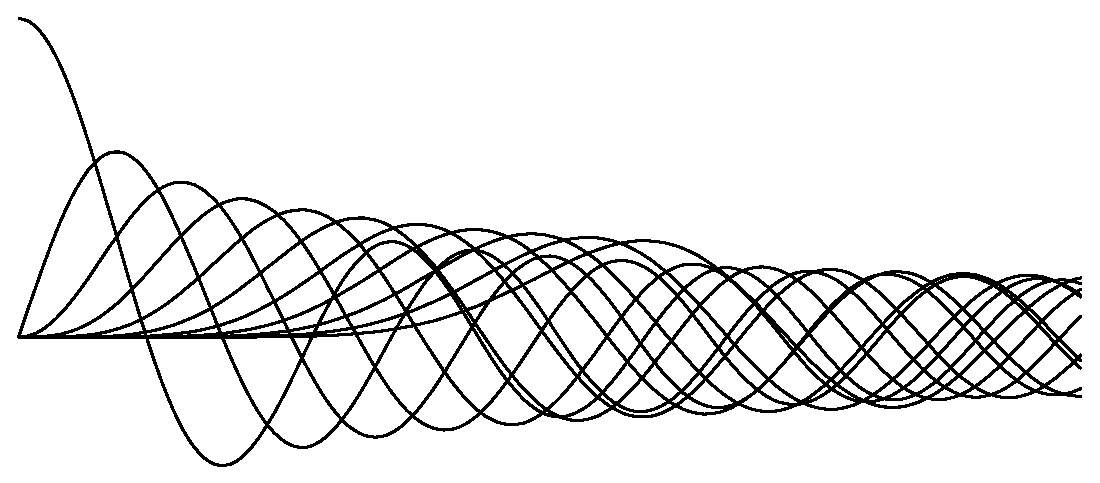
\includegraphics[width=10cm]{Bessel/Bessel.ps}
\end{center}

  この図には $0$ 次から $10$ 次までの Bessel 関数の、$[0,20]$ の範囲の
グラフを描いてある。いずれも振動しながら減衰していくのが分かる。

\subsection{零点を求める}

  Bessel 関数の零点をまとめて求めるための賢い方法もあるらしいが、
まだ読んでいないので、
ここではライブラリィ関数を使って方程式を解いて求めてみる
(ものすごい安直)。
なお桂田 \cite{桂田ベッセル} も参照せよ。

%
\begin{shaded}
 \footnotesize
 \verbatimfile{prog/find_Bessel_roots.c}
\end{shaded}

\begin{itembox}{$J_0$, $J_1$, $J_2$ の最初の 10 個の零点}
\verbatimfile{prog/find_Bessel_roots.out}
\end{itembox}

(後の (\ref{eq:漸化式2}) を使えば、
導関数が計算出来るので、Newton 法で計算できるはず。
今度遊んでみよう。)

\section{メモ}

\subsection{Bessel の積分, Hansen の積分}

$n\in\N_0$ とする。
\[
  J_n(z)
  =\sum_{m=0}^\infty\frac{(-1)^m}{m!(n+m)!}\left(\frac{z}{2}\right)^{n+2m}
\]
であるが、実は $C$ を原点のまわりを正の向きに一周する閉曲線とすると
\[
  J_n(z)=\frac{1}{2\pi i}\oint_{C}
         e^{(z/2)(\zeta-1/\zeta)}\frac{\D \zeta}{\zeta^{n+1}}
\]
が成り立つ。実際 $\zeta=2u/z$ と変数変換して得られる
\[
  \mbox{右辺}=\frac{1}{2\pi i}\sum_{m=0}^\infty\frac{(-1)^m}{m!}
  \left(\frac{z}{2}\right)^{n+2m}\oint_{C'}\frac{e^u}{u^{n+m+1}}\D u
\]
で、右辺の線積分を留数計算すれば $J_n(z)$ に等しいことが分かる。

これから
\[
  J_n(z)=\frac{1}{\pi}\int_0^\pi\cos(n\varphi-z\sin\varphi)\D\varphi
\]
が得られる。これを $J_n$ に対する \textbf{Bessel の積分}
(\textbf{Bessel's integral for $J_n$})とよぶ。

  要するに
\[
  e^{(z/2)(\zeta-1/\zeta)}=\sum_{n=-\infty}^{\infty}\zeta^n J_n(z).
  =J_0(z)+\sum_{n=1}^{\infty}\left[\zeta^n+(-1)^n\zeta^{-n}\right]J_n(z)
\]
が成立するわけで、
$e^{(z/2)(\zeta-1/\zeta)}$ は $J_n(z)$ の\textbf{母関数} (\textbf{generating
function}) である。

ちなみに、先に母関数表示
\[
 \exp\left[\frac{z}{2}\left(t-\frac{1}{t}\right)\right]
 =\sum_{n=-\infty}^\infty J_n(z)t^n
\]
からスタートして、$t=e^{i\theta}$ とおいて、
\[
 \cos(z\sin\theta),\quad \sin(z\cos\theta)
\]
の Fourier 級数展開を考えてもよい。

\begin{yodan}
  上式を
\[
  J_n(z)=\frac{1}{2\pi}\int_0^{2\pi}\cos(n\varphi-z\sin\varphi)\D\varphi
\]
と書き換えると、解析的周期関数の1周期にわたる積分なので、
台形公式で高精度に計算できる。
例えば $J_4(5)$ の計算に、
区間を (わずか) $32$ 等分した台形公式で $10^{-16}$ オーダーの
精度の値が得られる。 \qed
\end{yodan}

\subsection{加法定理}

(準備中)

\subsection{漸化式 (基本関係)}

  $J_\nu$ の級数による定義式から、単純な計算によって、
次の2つの漸化式 (recurrence formulae) が確かめられる。
\begin{align}
  &\frac{2\nu}{z}J_\nu(z)=J_{\nu-1}(z)+J_{\nu+1}(z),\label{eq:漸化式1}\\
  &2J_\nu'(z)=J_{\nu-1}(z)-J_{\nu+1}(z). \label{eq:漸化式2}
\end{align}

  $\nu=0$ の場合は特に $J_{-1}(z)=-J_1(z)$ であるから、
\[
  J_0'(z)=-J_1(z).
\]

(\ref{eq:漸化式1}), (\ref{eq:漸化式2}) を方程式とみなして解くと
\begin{align}
  &J_{\nu-1}(z)=\frac{n}{z}J_{\nu}(z)+J_{\nu}'(z),\label{eq:漸化式3}\\
  &J_{\nu+1}(z)=\frac{n}{z}J_{\nu}(z)-J_{\nu}'(z).\label{eq:漸化式4}
\end{align}
これらは次のように変形できる。
\begin{align}
  &\frac{\D}{\D z}\left(z^\nu J_\nu(z)\right)=z^\nu J_{\nu-1}(z),\\
  &\frac{\D}{\D z}\left(z^{-\nu}J_\nu(z)\right)=-z^{-\nu}J_{\nu+1}(z).
\end{align}
特に
\[
  \frac{\D}{\D z}\left(z J_1(z)\right)=z J_0(z).
\]

少なくとも次のことは言える。
\begin{center}
  Bessel 関数の導関数 (不定積分) は番号をずらしたりして簡単に計算できる。
\end{center}

\begin{yodan}
  少数の Bessel 関数だけを使って他のものを表すこと。
\begin{enumerate}
\item
  次数の低いもので表す。
  (\ref{eq:漸化式3}) により、
$J_{\nu+1}$ は $J_{\nu}$ と $J_{\nu}'$ で表現できるわけだが、
$J_{\nu}$ は 2 階の微分方程式の解であるから、
$J_{\nu+1}$ の導関数達も $J_{\nu}$ と $J_{\nu}'$ で表現できることが分かる:
\[
  \forall k\in\N_0\quad\exists P(t),Q(t)\in\C[t]\quad\mbox{s.t.}\quad
  \left(\frac{\D}{\D z}\right)^k J_{\nu+1}(z)
  =P\left(\frac{1}{z}\right) J_\nu(z)+Q\left(\frac{1}{z}\right) J_\nu'(z).
\]
\item
  次数の高いもので表す。
\[
  \forall k\in\N_0\quad\exists
  \widetilde P(t),\widetilde Q(t)\in\C[t]\quad\mbox{s.t.}\quad
  \left(\frac{\D}{\D z}\right)^k J_{\nu-1}(z)
  =\widetilde P\left(\frac{1}{z}\right) J_\nu(z)
   +\widetilde Q\left(\frac{1}{z}\right) J_\nu'(z).
\]
\item
  (上の二つを使うと)
  例えば $\nu=n\in\Z$ のとき、$J_n(z)$ とそのすべての導関数は
\[
   P\left(\frac{1}{z}\right) J_0(z)+Q\left(\frac{1}{z}\right) J_0'(z)
  =P\left(\frac{1}{z}\right) J_0(z)-Q\left(\frac{1}{z}\right) J_1(z)
\]
の形に表現できる
(数式処理を使うと少し遊べそう)。 \qed
\end{enumerate}
\end{yodan}

\subsection{半整数次数の Bessel 関数}

(準備中)

すでに $J_{\pm 1/2}$, $J_{\pm3/2}$ が
三角関数を用いて表されることは紹介済みである
((\ref{eq:1/2のBessel関数1}), (\ref{eq:1/2のBessel関数2}))。
漸化式
\[
  J_{\nu-1}(x)+J_{\nu+1}(x)=\frac{2\nu}{x}J_\nu(x)
 \quad\text{($x>0$)}
\]
が成り立つので、帰納法で、
任意の $n=0,1,2,\cdots$ に対して、
有理関数 $P_n(x)$, $Q_n(x)$ が存在して、
\[
  J_{n\pm 1/2}(x)
 =\frac{1}{\sqrt{\pi x}}\left(P_n(x)\cos x
+Q_n(x)\sin x\right)
\]
が得られる。

\subsection{漸近挙動}

(準備中 --- 既に簡単な結果だけは紹介してあるが…)

\section{変形 Bessel 関数}

  円柱で Laplace 方程式を解く際に現れる変形 Bessel 関数を導入する。

  この節では、 $i$ で虚数単位を表す ($i^2=-1$)。

  $\nu\in\C$ に対して、
\begin{equation}
  u''+\frac{1}{z}u'-\left(1+\frac{\nu^2}{z^2}\right)u=0
  \label{eq:変形Bessel方程式}
\end{equation}
を $\nu$ 次の\textbf{変形 Bessel の方程式}とよぶ。

カッコ内の $1$ を $-1$ に置き換えると通常の Bessel の微分方程式になる。
このことから、特解として $J_\nu(iz)$, $Y_{\nu}(iz)$ があることが分かるが、
応用上は、$z=x\in\R$ とするときに実数値となる解が望ましい。
少し考えると、正則な解として
\[
  I_\nu(z):=e^{-\nu\pi i/2}J_\nu(i z)=
  \left(\frac{z}{2}\right)^{\nu}
  \sum_{m=0}^\infty
  \frac{1}{m!\itGamma(\nu+m+1)}\left(\frac{z}{2}\right)^{2m}
\]
が得られる。これを $\nu$ 次の\textbf{変形 Bessel 関数} (\textbf{modified
Bessel function of the first kind of
order $\nu$}) という\footnote{というわけで、
複素変数の Bessel 関数 $J_\nu$ について完全な知識が得られれば、
わざわざ $I_\nu$ を持ち出す必要はない、ということになる。}。
特に $\nu=n\in\N_0$ の場合は
\[
 I_n(z)=i^{-n}J_n(iz)
\]
である。例えば
\[
  I_{1/2}(z)=\left(\frac{2}{\pi z}\right)^{1/2}\sinh z,\quad
  I_{-1/2}(z)=\left(\frac{2}{\pi z}\right)^{1/2}\cosh z.
\]

  Bessel 関数と同様に、
\begin{align*}
  &\det\left(\begin{array}{rr} I_{\nu}(z) & I_{-\nu}(z) \\ I_{\nu}'(z) &
 I_{-\nu}'(z) \end{array}\right)
  =I_\nu(z)I_{-\nu}'(z)-I_{\nu}'(z)I_{-\nu}(z)=-\frac{2\sin\nu\pi}{\pi z},\\
  &I_{-n}(z)=I_n(z)\quad\mbox{($n\in\N$)}
\end{align*}
が成り立つ。ゆえに $\nu\not\in\Z$ の場合、
\[
 u=C_1 I_{\nu}(z)+C_2 I_{-\nu}(z)\quad\mbox{($C_1$, $C_2$ は任意定数)}
\]
は変形 Bessel の方程式の一般解を与えるが、
$\nu\in\Z$ の場合はそうならない。

  そこで $\nu\not\in\Z$ の場合、
\[
 K_\nu(z):=\frac{\pi}{2}\frac{I_{-\nu}(z)-I_\nu(z)}{\sin\nu\pi},
\]
  $\nu=n\in\Z$ の場合、
\[
  K_n(z)=\lim_{\nu\to n}K_{\nu}(z)
 =\frac{(-1)^n}{2}\left.\left(\frac{\rd I_{-\nu}}{\rd\nu}(z)-
\frac{\rd I_\nu}{\rd\nu}(z)\right)\right|_{\nu=n}
\]
とおくことによって $K_{\nu}(z)$ を定める\footnote{不定形の極限なので、
ロピタルの定理が適用できることに注意しよう。}。こうすると
\[
 y=C_1 I_\nu(z)+C_2 K_\nu(z)
 \quad\mbox{($C_1$, $C_2$ は任意定数)}
\]
は (\ref{eq:変形Bessel方程式}) の一般解になる。

$k\ne 0$ に対して、微分方程式
\[
   u''+\frac{1}{z}u'-\left(k^2+\frac{\nu^2}{z^2}\right)u=0
\]
の一般解は
\[
 y=C_1 I_\nu(k z)+C_2 K_\nu(k z)
 \quad\mbox{($C_1$, $C_2$ は任意定数)}.
\]

\begin{yodan}
  Kelvin 卿により導入された $\mathrm{ber}\;x$, $\mathrm{bei}\; x$ という
関数があるが、これは
\[
  I_0\left(\frac{1+i}{\sqrt{2}}x\right)
  =\mathrm{ber}\;x+i\;\mathrm{bei}\;x
\]
で定義される。
\begin{align*}
  &\mathrm{ber}\;x
   =1-\frac{x^4}{2^2\cdot 4^2}+\frac{x^8}{2^2\cdot4^2\cdot6^2\cdot8^2}-\cdots\\
  &\mathrm{bei}\;x
   =\frac{x^2}{2^2}-\frac{x^6}{2^2\cdot 4^2\cdot 6^2}
   +\frac{x^{10}}{2^2\cdot4^2\cdot6^2\cdot8^2\cdot10^2}-\cdots  \qed
\end{align*}
\end{yodan}

\section{Bessel について}

Friedrich Wilhelm Bessel (1784--1846, Minden に生まれ、
K\"onigsberg にて没する, 天文学に顕著な業績がある) は、
Kepler の方程式を解くために Bessel 関数の基礎固めをすることになった。

\subsection*{Bessel の問題}

太陽の回りを1つの惑星がまわる二体問題を考える。
楕円軌道が $(x/a)^2+(y/b)^2=1$ で、
焦点 $(c,0)$ ($c=\sqrt{a^2-b^2}$) に太陽があるとする。
近日点 $(a,0)$ が $\pi=(1,0)$ となるように縮尺を変えると、
太陽の位置は $\mathrm{S}=(e,0)$ となる ($e=c/a$)。
単位円周上を等角速度で動く仮想の天体を考える。
ただし、周期と近日点を過ぎるタイミングは問題としている惑星と同じとする。
ある時刻に平均近点角が $M$ であるとは、
その仮想の天体の座標が $(\cos M,\sin M)$ ということである。
問題の惑星の位置を $\mathrm{P}=(x,y)$ とする。
単位円周上の点 $\mathrm{P}'$ を $\mathrm{P}'=(x,
\sqrt{1-x^2}\,\sign y)$ で定める。
$E=\angle \pi\mathrm{OP}'$ を離心近点角という。
Kepler の法則から、
離心近点角 (eccentric anomaly) $E$, 平均近点角 (mean anomaly) $M$,
楕円の離心率 (eccentricity) $e\in[0,1)$ について
%
\begin{equation}
  E-e\sin E=M
  \label{eq:ケプラーの方程式}
\end{equation}
%
という関係式が成り立つ。これを \textbf{Kepler の方程式}とよぶ
(これは文献に初めて現れた超越方程式という評判がある)。
この方程式を解いて $E$ や $\cos(m E)$, $\sin(m E)$ を $M$ で
表すことを \textbf{Bessel の問題}という。

これを解くために Bessel 関数が必要になった、ということである。
実際、解は
\begin{align}
  &E=M+\sum_{n=1}^\infty\frac{2}{n}J_n(ne)\sin(nM),\\
  &\cos(m E)=-\frac{e}{2}\delta_{m1}+\sum_{n=1}^\infty
  \frac{m}{n}\left(J_{n-m}(ne)+J_{n+m}(ne)\right)\cos(n M),\\
  &\sin(m E)=
  \sum_{n=1}^\infty\frac{m}{n}\left(J_{n-m}(ne)+J_{n+m}(ne)\right)\sin(n M)
\end{align}
と表される。

なお、$E$ から真近点角 (true anomaly) $\angle\pi\mathrm{SP}=\nu$ を求めるには、
方程式
\[
 \tan\frac{\nu}{2}=\sqrt{\frac{1+e}{1-e}}\tan\frac{E}{2}
\]
を解けばよい。

\begin{yodan}[Kepler の方程式を数値的に解く]
具体的に数値で与えられた $M$, $e$ に対して、
(\ref{eq:ケプラーの方程式}) の解 $E$ を求めるには、
数値解法を使うのが簡単である。
筆者は初めてパソコンを買った頃に遊んでいた天文計算プログラム
(中野主一氏作) の中でこの方程式に出会い、
「(Kepler の方程式を解くと言っても、
微分方程式を解いているわけではないし) 一体何をしているのだろう?」
と不思議に思った経験がある。 \qed
\end{yodan}

\chapter{Laplacian の極座標表示}

\section{2次元の場合}\label{節:ラプラシアンの極座標表示}
  $\R^2$ における極座標
\begin{eqnarray*}
  &&x=r\cos\theta,\\
  &&y=r\sin\theta
\end{eqnarray*}
で Laplacian を表すと
\begin{equation}
 \Laplacian
  = \frac{\rd^2}{\rd r^2}
   +\frac{1}{r}\frac{\rd}{\rd r}
   +\frac{1}{r^2}\frac{\rd^2}{\rd\theta^2}
  \label{eq:2次元ラプラシアンの極座標表示}
\end{equation}

この公式の導出は例えば、
桂田『解析概論I講義ノート』 \cite{桂田解析概論1}
(あるいはその改訂版 \cite{桂田多変数1}) に載せてある。
その要点は
\[
  \left(
  \begin{array}{cc}
  {x_r} & {x_\theta} \\
  {y_r} & {y_\theta}
  \end{array}
  \right)
 =
  \left(
  \begin{array}{cr}
  \cos\theta & -r\sin\theta \\
  \sin\theta &  r\cos\theta
  \end{array}
  \right)
\]
より
\[
  \left(
  \begin{array}{cc}
  {r_x} & {r_y} \\
  {\theta_x} & {\theta_y}
  \end{array}
  \right)
 =
  \left(
  \begin{array}{cc}
  {x_r} & {x_\theta} \\
  {y_r} & {y_\theta}
  \end{array}
  \right)^{-1}
 =
  \left(
  \begin{array}{cr}
  \cos\theta & -r\sin\theta \\
  \sin\theta &  r\cos\theta
  \end{array}
  \right)^{-1}
 =\frac{1}{r}
  \left(
  \begin{array}{rr}
   r\cos\theta & r\sin\theta \\
  -\sin\theta & \cos\theta
  \end{array}
  \right)
\]
であるから、
\begin{align*}
 \frac{\rd}{\rd x}
 =\frac{\rd r}{\rd x}\frac{\rd}{\rd r}
 +\frac{\rd\theta}{\rd x}\frac{\rd}{\rd\theta}
 =\cos\theta\frac{\rd}{\rd r}-\frac{\sin\theta}{r}\frac{\rd}{\rd\theta},\\
 \frac{\rd}{\rd y}
 =\frac{\rd r}{\rd y}\frac{\rd}{\rd r}
 +\frac{\rd\theta}{\rd y}\frac{\rd}{\rd\theta}
 =\sin\theta\frac{\rd}{\rd r}+\frac{\cos\theta}{r}\frac{\rd}{\rd\theta}.
\end{align*}
これから
\[
 \Laplacian u
 =\frac{\rd^2u}{\rd x^2}+\frac{\rd^2u}{\rd y^2}
 =\left(\cos\theta\frac{\rd}{\rd r}
       -\frac{\sin\theta}{r}\frac{\rd}{\rd\theta}\right)^2 u
  +\left(
     \sin\theta\frac{\rd}{\rd r}+\frac{\cos\theta}{r}\frac{\rd}{\rd\theta}
   \right)^2 u.
\]
後はこれをていねいに計算するだけである。

また付録の \ref{ch:楕円ラプラアシアン} 章「楕円領域のラプラシアン」に
この公式を数式処理で導出するための Mathematica プログラムを載せてある。

\section{3次元の場合}

\begin{align*}
 \Laplacian
 &=\frac{\rd^2}{\rd r^2}
  +\frac{2}{r}\frac{\rd}{\rd r}
  +\frac{1}{r^2}\Lambda,\\
  \Lambda&=\frac{1}{\sin\theta}
          \frac{\rd}{\rd\theta}
	  \left(
	  \sin\theta\frac{\rd}{\rd\theta}
	  \right)
          +\frac{1}{\sin^2\theta}
          \frac{\rd^2}{\rd\phi^2}
  =\frac{\rd^2}{\rd\theta^2}+\cot\theta\frac{\rd}{\rd\theta}
   +\frac{1}{\sin^2\theta}\frac{\rd^2}{\rd\phi^2}.
\end{align*}

この公式の導出も桂田『解析概論I講義ノート』 \cite{桂田解析概論1}
(あるいはその改訂版 \cite{桂田多変数1}),
『極座標とLaplacian』 \cite{桂田極座標} に載せてある。

Mathematica プログラムも書いてみたい。

はてな?$n=2$ のときを
\[
 \Laplacian=\frac{1}{r}\frac{\rd}{\rd r}\left(r\frac{\rd}{\rd r}\right)
  +\frac{1}{r^2}\frac{\rd^2}{\rd\theta^2}
\]
と書くと、何か不思議な感じがする (Laplacian も漸化式で書ける?)。

\section{一般の $n$ 次元の場合}

  $n$ 次元空間 $\R^n$ における Laplacian の極座標表示は、
島倉 \cite{島倉} にあったような記憶がある。

  $u(x)=f(r)$, $r=|x|$ となる場合は、
\[
  \Laplacian u=f''(r)+\frac{n-1}{r}f'(r)
\]
となる (「微分方程式2」の講義ノート (桂田 \cite{桂田1}) にも書いたが、
簡単であるので自力で確認するとよい)。

一般の場合は
\[
  \Laplacian u=\frac{1}{r^{n-1}}\frac{\rd}{\rd r}\left(r^{n-1}u_r\right)
   +\frac{1}{r^2}\Lambda u
  =u_{rr}+\frac{n-1}{r}u_r+\frac{1}{r^2}\Lambda u.
\]
  ここで $\Lambda$ は単位球面の \textbf{Laplace-Beltrami 作用素}である。

$n=2$ のときは
\begin{equation}
 \Lambda=\Lambda_\theta=\frac{\rd^2}{\rd\theta^2}.
 \label{eq:2次元ラプラス・ベルトラミ作用素}
\end{equation}
$n=3$ のときは
\begin{equation}
 \Lambda=\Lambda_{\theta,\phi}
 =\frac{1}{\sin\theta}\frac{\rd}{\rd\theta}
  \left(\sin\theta\frac{\rd}{\rd\theta}\right)
  +\frac{1}{\sin^2\theta}\frac{\rd^2}{\rd\phi^2}.
  \label{eq:3次元ラプラス・ベルトラミ作用素}
\end{equation}

\chapter{円盤領域における熱方程式}

  境界条件は同次の場合を考える。

\section{円盤領域での Dirichlet 境界値問題}\label{sec:円盤Dirichlet}
\label{sec:円盤領域における熱方程式のディリクレ問題}

2次元の単位円盤領域
\[
 \Omega:=\{(x,y)\in\R^2; x^2+y^2<1\}
\]
における熱方程式の初期値境界値問題
\begin{equation}
 u_t=\Laplacian u,\quad u(x,y,t)=0\quad\mbox{($(x,y)\in\rd\Omega$)},\quad
 u(x,y,0)=u_0(x,y)\quad\mbox{($(x,y)\in\overline\Omega$)}
 \label{eq:円盤における初期値ディリクレ境界値問題}
\end{equation}
を Fourier の方法で解いてみよう。

いつものように、
熱方程式と境界条件を満たし、
$u(x,y,t)=\eta(t)\zeta(x,y)$ という形をしている
非自明な $u$ を求めることを目標にする。
まず熱方程式に代入すると
%
\[
  \frac{\Laplacian\zeta(x,y)}{\zeta(x,y)}
 =\frac{\eta'(t)}{\eta(t)}.
\]
これは定数なので $-\lambda$ とおくと、
\[
 \eta'(t)=-\lambda\eta(t),
 \quad
 \Laplacian\zeta(x,y)=-\lambda\zeta(x,y).
\]

一方、境界条件に代入すると
\[
 \zeta(x,y)=0\quad\mbox{($(x,y)\in\rd\Omega$)}
\]
を得る。

  こうして、$\Omega$ における Laplacian の固有値問題が登場する。

  $\Omega$ は、
$1$ 次元区間の直積ではないから、
このままでは Fourier の方法は適用できないが、
極座標を用いて問題を変換するとうまく解けるようになる。
%
\begin{align*}
   x&= r\cos\theta,\\
   y&= r\sin\theta
\end{align*}
%
により変数を $(x,y)$ から $(r,\theta)$ に変換し、
\[
  Z(r,\theta):=\zeta(x,y)
\]
とおくと、$-\Laplacian \zeta=\lambda\zeta$ は
%
\[
  \frac{\rd^2 Z}{\rd r^2}+\frac{1}{r}\frac{\rd Z}{\rd r}+
  \frac{1}{r^2}\frac{\rd^2 Z}{\rd\theta^2}=-\lambda\zeta
  \quad\mbox{($0<r<1$, $\theta\in[0,2\pi]$)}
\]
%
という方程式に変換される。ここで
%
\[
  Z(r,\theta)=R(r)\Theta(\theta)
\]
%
とおいて、代入すると
%
\[
   R''(r)\Theta(\theta)
 +\frac{1}{r}R'(r)\Theta(\theta)
 +\frac{1}{r^2}R(r)\Theta''(\theta)
 =-\lambda R(r)\Theta(\theta).
\]
%
  両辺を $R(r)\Theta(\theta)$ で割って、
%
\[
   \frac{R''(r)}{R(r)}
 +\frac{1}{r}\frac{R'(r)}{R(r)}
 +\frac{1}{r^2}\frac{\Theta''(\theta)}{\Theta(\theta)}
 =-\lambda.
\]
%
移項すると
\[
  \frac{r^2 R''(r)+r R'(r)+\lambda r^2 R(r)}{R(r)}=
  -\frac{\Theta''(\theta)}{\Theta(\theta)}.
\]
%
(いつものように) この式の値は定数であることが分る。
それを $\alpha$ とおくと、
\begin{align*}
 &\Theta''(\theta)+\alpha\Theta(\theta)=0,\\
 &r^2 R''(r)+r R'(r)+\left(\lambda r^2-\alpha\right)R(r)=0.
\end{align*}
  $\Theta$ は周期 $2\pi$ の関数であるから\footnote{任意の $k\in\Z_{\ge 0}$
に対して $\Theta^{(k)}(0)=\Theta^{(k)}(2\pi)$ が成り立つが、
微分方程式から $k=0,1$ のときだけ考えれば良いことが分かる。}、
\[
  \Theta(0)=\Theta(2\pi),\quad \Theta'(0)=\Theta'(2\pi).
\]
こうして $\Theta$ についての固有値問題
\begin{equation}
  \Theta''(\theta)=-\alpha\Theta(\theta),\quad
  \Theta(0)=\Theta(2\pi),\quad \Theta'(0)=\Theta'(2\pi)
\end{equation}
が導かれた。これは (よく知られているように)
\begin{equation}
 \alpha=n^2,\quad n\in\N\cup\{0\},\quad
 \Theta(\theta)=A\cos n\theta+B\sin n\theta
  \quad\mbox{($A$, $B$ は任意定数)}
\end{equation}
と解ける。一方 $R$ については、境界条件も考慮して
\begin{equation}
  R'(r)+\frac{1}{r}R'(r)+\left(\lambda-\frac{n^2}{r^2}\right)R(r)=0,\quad
  R(1)=0,\quad \mbox{$R(0)$ は有限}.
\end{equation}
多くの本で、この形で条件を書いてあるが、固有値問題であるから
\begin{equation*}
  R'(r)+\frac{1}{r}R'(r)-\frac{n^2}{r^2}R(r)=-\lambda R(r),\quad
  R(1)=0,\quad \mbox{$R(0)$ は有限}.
\end{equation*}
と書く方が良いかもしれない。

  ここで
\[
  \rho:=\sqrt{\lambda}r,\quad W(\rho):=R(r)
\]
とおくと $R(r)=W\left(\sqrt{\lambda}r\right)$ より、
\[
  R'(r)=\sqrt{\lambda}W(\rho),\quad R''(r)=\lambda W''(\rho)
\]
であるから、上の方程式に代入して、
\begin{subequations} % 2021-04-31 00:23の式群
\begin{align}
 &W''(\rho)+\frac{1}{\rho}W'(\rho)+\left(1-\frac{n^2}{\rho^2}\right)W(\rho)=0,
 \label{eq:Besselの方程式登場} \\
 &W\left(\sqrt{\lambda}\right)=0,\quad\mbox{$W(0)$ は有限}.
 \label{eq:Wに関する境界条件}
\end{align}
\end{subequations}
  
  (\ref{eq:Besselの方程式登場}) は Bessel の微分方程式である。一般解は
\[
  W(\rho)=A J_n(\rho)+B Y_n(\rho)\quad\mbox{($A$, $B$は任意定数)}
\]
である (定理\ref{jtheorem:ベッセルの微分方程式の一般解})。
ここで $J_n$ は $n$ 次の Bessel 関数、
$Y_n$ は $n$ 次の Neumann 関数である。
\[
  J_n(z):=\sum_{k=0}^\infty\frac{(-1)^k}{k! (n+k)!}
 \left(\frac{z}{2}\right)^{n+2k}.
\]
  $Y_n$ については、原点の近傍で有界でないこと以外は使わないので、
ここでは定義式は省略する
 (定義\ref{jtheorem:ベッセルの微分方程式の一般解} を見よ)。

原点の近傍で $W$ は有界であることから、$B=0$ でなければならない。すなわち
\[
 W(\rho)=A J_n(\rho).
\]
ゆえに
\[
  R(r)=A J_n(\sqrt{\lambda}r).
\]

  $R(1)=0$ であるためには、
$\sqrt{\lambda}$ は $J_n$ の零点であることが必要十分である。

$J_n$ の正の零点は小さい方から順に並べることができる
(どこかに集積したりはしない)。
それを
\[
  \mu_{1,n}<\mu_{2,n}<\cdots<\mu_{m,n}<\cdots
\]
とおくと、
\[
  \exists m\in\N\quad\mbox{s.t.}\quad \sqrt{\lambda}=\mu_{m,n}.
\]
以上から円盤における固有値問題の解として
\begin{equation}
  \lambda=\mu_{m,n}^2,\quad
  Z(r,\theta)=J_n(\mu_{m,n}r)
  \left\{
   \begin{matrix}
     \cos n\theta\\ \sin n\theta
   \end{matrix}
  \right\}
\end{equation}
が得られる。

ゆえに円盤における熱方程式に対する変数分離解として
\[
 e^{-\mu_{m,n}^2 t}
 J_n(\mu_{m,n}r)
    \left\{
   \begin{matrix}
     \cos n\theta\\ \sin n\theta
   \end{matrix}
  \right\}
\]
が得られる。

初期値境界値問題 (\ref{eq:円盤における初期値ディリクレ境界値問題}) の解は、
それらの重ね合わせ
\begin{equation}
 u(x,y,t)
  =\frac{1}{2}\sum_{m=1}^\infty A_{m0}e^{-\mu_{m,0}^2 t}J_0(\mu_{m,0}r)
 +\sum_{n=1}^\infty\sum_{m=1}^\infty
  e^{-\mu_{m,n}^2 t}
 J_n(\mu_{m,n}r)(A_{mn}\cos n\theta+B_{mn}\sin n\theta)
\end{equation}
で与えられると期待できる。係数 $A_{mn}$, $B_{mn}$ は、
定理\ref{jtheorem:フーリエ・ベッセルの展開}より
\begin{subequations} % 2021-04-31 00:34の式群
\begin{align}
 &A_{mn}=\frac{2}{\pi J_{n+1}(\mu_{mn})^2}
  \int_0^1\left(\int_{-\pi}^{\pi}f(r,\theta)\cos n\theta\;\D\theta\right)
    r J_n(\mu_{m,n}r)\D r,\\
 &B_{mn}=\frac{2}{\pi J_{n+1}(\mu_{mn})^2}
  \int_0^1\left(\int_{-\pi}^{\pi}f(r,\theta)\sin n\theta\;\D\theta\right)
    r J_n(\mu_{m,n}r)\D r.
\end{align}
\end{subequations}

\iffalse
\begin{yodan}
  公式の書き方だが、$n=0$ とそうでないのを分けるのは面倒なので、
\begin{align*}
 &u(r\cos\theta,r\sin\theta,t)
  =\sum_{n=0}^\infty\sum_{m=1}^\infty
  e^{-\mu_{m,n}^2 t}
 J_n(\mu_{m,n}r)(A_{mn}\cos n\theta+B_{mn}\sin n\theta),\\
 &A_{mn}=\frac{\eps_n}{\pi J_{n+1}(\mu_{mn})^2}\int_0^1 r J_n(\mu_{m,n}r)\D r
  \int_{-\pi}^{\pi}f(r,\theta)\cos n\theta\;\D\theta,\\
 &
 B_{mn}=\frac{\eps_n}{\pi J_{n+1}(\mu_{mn})^2}\int_0^1 r J_n(\mu_{m,n}r)\D r
  \int_{-\pi}^{\pi}f(r,\theta)\sin n\theta\;\D\theta,\\
 &\eps_n=\left\{
  \begin{array}{ll}
   2 & \mbox{($n\ne 0$)}\\
   1 & \mbox{($n=0$)}
  \end{array}
  \right.
\end{align*}
くらいがよいだろうか?それとも $\eps_n$ を $2-\delta_{n0}$ と書くか? \qed
\end{yodan}
\fi

\section{円盤領域での Neumann 境界値問題}

(工事中…卒研でのチャレンジャー募集中)

金子 \cite{金子} に Neumann 境界値問題についての言及がある
(熱方程式ではなく、波動方程式だが、固有関数はまったく同じわけだから)。
\begin{align*}
  &u_t(x,y,t)=\Laplacian u(x,y,t)\quad\mbox{($(x,y)\in\Omega$,  $t>0$)},\\
  &\frac{\rd u}{\rd n}(x,y,t)=0 \quad\mbox{($(x,y)\in\rd\Omega$, $t>0$)},\\
  &u(x,y,0)=f(x,y) \quad\mbox{($(x,y)\in\overline\Omega$)}.
\end{align*}

最初の素朴な予想は、式の形は Dirichlet 境界条件の場合と同じで、
\[
 u(r\cos\theta,r\sin\theta,t)
  =\frac{1}{2}\sum_{m=1}^\infty A_{m0}e^{-\mu_{m,0}^2 t}J_0(\mu_{m,0}r)
 +\sum_{n=1}^\infty\sum_{m=1}^\infty
  e^{-\mu_{m,n}^2 t}
 J_n(\mu_{m,n}r)(A_{mn}\cos n\theta+B_{mn}\sin n\theta).
\]
\[
 A_{mn}=\frac{2}{\pi J_{n+1}(\mu_{mn})^2}\int_0^1
  \left(int_{-\pi}^{\pi}f(r,\theta)\cos n\theta\;\D\theta\right)
   r J_n(\mu_{m,n}r)\D r.
\]
\[
 B_{mn}=\frac{2}{\pi J_{n+1}(\mu_{mn})^2}\int_0^1
   \left(\int_{-\pi}^{\pi}f(r,\theta)\sin n\theta\;\D\theta\right)
   r J_n(\mu_{m,n}r)\D r.
\]
ただし $\mu_{m,n}$ は $J_n'(x)$ の零点を順番に小さい方から順に
並べたものである?
\[
  \mu_{1,n}<\mu_{2,n}<\mu_{3,n}<\cdots<\mu_{m,n}<\mu_{m+1,n}<\cdots
\]
  (この $\mu_{m,n}$ をもう少し具体的に書けないかなとも思うけれど、
仕方がないのだろうか?)

おっと、でも固有値 $\lambda=0$ というのがあるかな?
\begin{equation}
  R''+\frac{1}{r}R'+\left(0-\frac{n^2}{r^2}\right)R=0.
  \label{eq:λ=0の場合}
\end{equation}
に対して、$W(\rho)=R(r/\sqrt{0})$ という変数変換はできないから、
これは別途考察を要する、だな。
(\ref{eq:λ=0の場合}) は Euler の方程式か。
何だ、円盤で Laplace 方程式を解くときと同じだ
(例えば桂田 \cite{桂田1} の第3章)。一般解は
\[
 R(r)=\left\{
 \begin{array}{ll}
  A r^n+B r^{-n} & \mbox{($n\ne 0$)} \\
  A+B\log r & \mbox{($n=0$)}
  \end{array}
 \right.
\]
これで $R'(1)=0$ を満たすものを求めると、
\[
 R(r)=\left\{
 \begin{array}{ll}
  A\left(r^n-r^{-n}\right) & \mbox{($n\ne 0$)} \\
  A & \mbox{($n=0$)}
  \end{array}
 \right.
\]
なるほど。これは $m=0$ に対応するものと考えるべきかな。

きちんと計算して解を書き下す、
もちろん $\mu_{m,n}$ の漸近挙動の解析もつけて、
というのは、ちょっとした課題になるだろう。

$m$, $n$ が小さい (特に一方が $0$) 場合の変数分離解を可視化してみたい。

\chapter{円柱領域における熱方程式}

  境界条件は Dirichlet 境界条件とする
(Neumann や Robin どうなるのかなあ…)。

  この章の内容は吉原君の卒業研究レポートである。
まだチェックが入っていない。小さなミスはあると思うが、
大筋は正しいのでは?と考えている。

\section{同次 Dirichlet 境界条件の場合}

  これは寺沢 \cite{寺沢2} にある。後で照合してみよう。

半径 $1$, 高さ $h$ の円柱領域 $\Omega=\{(x,y,z); x^2+y^2<1,\ 0<z<h\}$ に
おける熱方程式の初期値境界値問題
\begin{align*}
  u_t(x,y,z,t)&=\Laplacian u(x,y,z,t) &&\mbox{($(x,y,z)\in\Omega$, $t>0$)},\\
  u(x,y,z,t)&=0 &&\mbox{($(x,y,z)\in\rd\Omega$, $t>0$)},\\
  u(x,y,z,0)&=f(x,y,z) &&\mbox{($(x,y)\in\overline\Omega$)}
\end{align*}
を考える。

\begin{align*}
  u(r\cos\theta,r\sin\theta,t)
 =\sum_{n=0}^\infty\sum_{m=1}^\infty
  e^{-((\ell\pi/h)^2+\mu_{mn}^2)t}
  J_n(\mu_{mn}r)(A_{\ell m n}\cos n\theta+B_{\ell m n}\sin n\theta)
   \sin\frac{\ell\pi z}{h},
\end{align*}
\begin{align*}
  A_{\ell m n}=\frac{4}{\pi h J_{n+1}(\mu_{mn})^2}
  \int_0^h\int_{-\pi}^\pi\int_0^1 r J_n(\mu_{mn}r)
  f(r\cos\theta,r\sin\theta,z)\cos n\theta\sin\frac{\ell\pi z}{h}\;
  \D r\,\D\theta\,\Dz,\\
  B_{\ell m n}=\frac{4}{\pi h J_{n+1}(\mu_{mn})^2}
  \int_0^h\int_{-\pi}^\pi\int_0^1 r J_n(\mu_{mn}r)
  f(r\cos\theta,r\sin\theta,z)\sin n\theta\sin\frac{\ell\pi z}{h}\;
  \D r\,\D\theta\,\Dz.
\end{align*}

  $n=0$ のとき、本当にこれでいいのか???

\section{非同次 Dirichlet 境界条件}

  非同次 Dirichlet 境界条件 (ただしデータは時刻 $t$ に依存しない) を
与えてみる。これは Laplace 方程式の Dirichlet 境界値問題を解けばよい。

  $\Gamma_s$ は側面、$\Gamma_t$ は上の面、$\Gamma_b$ は底の面とする。
\begin{align*}
  \Gamma_s&:=\{(x,y,z); x^2+y^2=1, 0<z<h\},\\
  \Gamma_t&:=\{(x,y,h); x^2+y^2<1\},\\
  \Gamma_b&:=\{(x,y,0); x^2+y^2<1\}.
\end{align*}

\subsection{側面で非同次データ}

\begin{align*}
  &\Laplacian u=0\quad\mbox{(in $\Omega$)},\\
  &u(x,y,z)=\Phi(x,y,z)\quad\mbox{($(x,y,z)\in\Gamma_s$)},\\
  &u(x,y,z)=0\quad\mbox{($(x,y,z)\in\Gamma_t\cup\Gamma_b$)}.
\end{align*}

この問題の解は変形Bessel 関数 $I_n$ を用いて、次のように与えられる。
\[
  u(r\cos\theta,r\sin\theta,z)
 =\sum_{n=0}^\infty\sum_{\ell=1}^\infty
  I_n\left(\frac{\ell\pi}{h}\right)
  \left(A_{\ell n}\cos n\theta+B_{\ell n}\sin
 n\theta\right)\sin\frac{\ell\pi z}{h},
\]
\[
 A_{\ell n}=\frac{2}{\pi h I_n(\ell\pi/h)}\int_0^h\int_{-\pi}^\pi
  \Phi(\cos\theta,\sin\theta,z)\cos n\theta\sin\frac{\ell\pi z}{h}\;
  \D\theta\,\D z,
\]
\[
 B_{\ell n}=\frac{2}{\pi h I_n(\ell\pi/h)}\int_0^h\int_{-\pi}^\pi
  \Phi(\cos\theta,\sin\theta,z)\sin n\theta\sin\frac{\ell\pi z}{h}\;
  \D\theta\,\D z.
\]

\subsection{上面で非同次データ}

\begin{align*}
  &\Laplacian u=0\quad\mbox{(in $\Omega$)},\\
  &u(x,y,z)=\Phi(x,y)\quad\mbox{($(x,y,z)\in\Gamma_t$)},\\
  &u(x,y,z)=0\quad\mbox{($(x,y,z)\in\Gamma_s\cup\Gamma_b$)}.
\end{align*}

\[
 u(r\cos\theta,r\sin\theta,z)=\sum_{n=0}^\infty\sum_{m=1}^\infty
  \sinh(\mu_{mn}z)J_n(\mu_{mn}r)
  \left(A_{mn}\cos n\theta+B_{mn}\sin n\theta\right),
\]
\[
 A_{mn}=\frac{2}{\pi\sinh(\mu_{mn}h)J_{n+1}(\mu_{mn})^2}
 \int_{-\pi}^\pi\int_0^1 r
  J_n(\mu_{mn}r)\Phi(r\cos\theta,r\sin\theta)\cos n\theta\;\D r\,\D\theta.
\]
\[
 B_{mn}=\frac{2}{\pi\sinh(\mu_{mn}h)J_{n+1}(\mu_{mn})^2}
 \int_{-\pi}^\pi\int_0^1 r
  J_n(\mu_{mn}r)\Phi(r\cos\theta,r\sin\theta)\sin n\theta\;\D r\,\D\theta.
\]

\subsection{底面で非同次データ}

\begin{align*}
  &\Laplacian u=0\quad\mbox{(in $\Omega$)},\\
  &u(x,y,z)=\Phi(x,y)\quad\mbox{($(x,y,z)\in\Gamma_b$)},\\
  &u(x,y,z)=0\quad\mbox{($(x,y,z)\in\Gamma_s\cup\Gamma_t$)}.
\end{align*}

\[
 u(r\cos\theta,r\sin\theta,z)=\sum_{n=0}^\infty\sum_{m=1}^\infty
  \sinh(\mu_{mn}(h-z))J_n(\mu_{mn}r)
  \left(A_{mn}\cos n\theta+B_{mn}\sin n\theta\right),
\]
\[
 A_{mn}=\frac{2}{\pi\sinh(\mu_{mn}h)J_{n+1}(\mu_{mn})^2}
 \int_{-\pi}^\pi\int_0^1 r
  J_n(\mu_{mn}r)\Phi(r\cos\theta,r\sin\theta)\cos n\theta\;\D r\,\D\theta.
\]
\[
 B_{mn}=\frac{2}{\pi\sinh(\mu_{mn}h)J_{n+1}(\mu_{mn})^2}
 \int_{-\pi}^\pi\int_0^1 r
  J_n(\mu_{mn}r)\Phi(r\cos\theta,r\sin\theta)\sin n\theta\;\D r\,\D\theta.
\]

\chapter{円盤領域における波動方程式}

  金子 \cite{金子} に少し詳しく書いてあったような記憶がある。
照合してみること。

  境界条件は同次 Dirichlet の場合を考える。

\section{Dirichlet 境界条件の場合}

  単位円盤 $\Omega=\{(x,y);x^2+y^2<1\}$ における
波動方程式の初期値境界値問題
\begin{align*}
  \frac{1}{c^2}u_{tt}
    &=\Laplacian u\quad\mbox{(in $\Omega\times(0,\infty)$)},\\
  u(x,t)&= 0\quad\mbox{(on $\rd\Omega\times(0,\infty)$)},\\
  u(x,0)&= \phi(x)\quad\mbox{($x\in\overline\Omega$)},\\
  u_t(x,0)&= \psi(x)\quad\mbox{($x\in\overline\Omega$)}
\end{align*}
の解は
\begin{align*}
 u
 &=\frac{1}{2}\sum_{m=1}^\infty
  A_{0m}J_0(\mu_{m0}r)\cos(c\mu_{m0}t)
  +\sum_{n=1}^\infty\sum_{m=1}^\infty
   J_n(\mu_{mn}r)\cos(c\mu_{mn}t)
  \left(A_{mn}\cos n\theta+B_{mn}\sin n\theta\right)\\
 &\!\!\!\!+
  \frac{1}{2}\sum_{m=1}^\infty
  C_{0m}J_0(\mu_{m0}r)\frac{\sin(c\mu_{m0}t)}{\mu_{m0}}
  +\sum_{n=1}^\infty\sum_{m=1}^\infty
   J_n(\mu_{mn}r)\frac{\sin(c\mu_{mn}t)}{\mu_{mn}}
  \left(C_{mn}\cos n\theta+D_{mn}\sin n\theta\right).
\end{align*}

\[
 A_{mn}=\frac{2}{\pi J_{n+1}(\mu_{mn})^2}\int_0^1 r J_n(\mu_{mn}r)\D r
  \int_{-\pi}^{\pi}\phi(r\cos\theta,r\sin\theta)\cos n\theta\;\D\theta.
\]
\[
 B_{mn}=\frac{2}{\pi J_{n+1}(\mu_{mn})^2}\int_0^1 r J_n(\mu_{mn}r)\D r
  \int_{-\pi}^{\pi}\phi(r\cos\theta,r\sin\theta)\sin n\theta\;\D\theta.
\]
\[
 C_{mn}=\frac{2}{\pi J_{n+1}(\mu_{mn})^2}\int_0^1 r J_n(\mu_{mn}r)\D r
  \int_{-\pi}^{\pi}\psi(r\cos\theta,r\sin\theta)\cos n\theta\;\D\theta.
\]
\[
 D_{mn}=\frac{2}{\pi J_{n+1}(\mu_{mn})^2}\int_0^1 r J_n(\mu_{mn}r)\D r
  \int_{-\pi}^{\pi}\psi(r\cos\theta,r\sin\theta)\sin n\theta\;\D\theta.
\]

あるいは上の余談の真似をして
\begin{align*}
 &u(r\cos\theta,r\sin\theta,t)
  =\sum_{n=0}^\infty\sum_{m=1}^\infty
   J_n(\mu_{mn}r)\cos(c\mu_{mn}t)
  \left(A_{mn}\cos n\theta+B_{mn}\sin n\theta\right)\\
 &\qquad\qquad+\sum_{n=0}^\infty\sum_{m=1}^\infty
   J_n(\mu_{mn}r)\frac{\sin(c\mu_{mn}t)}{\mu_{mn}}
  \left(C_{mn}\cos n\theta+D_{mn}\sin n\theta\right),\\
 &A_{mn}=\frac{2-\delta_{n0}}{\pi J_{n+1}(\mu_{mn})^2}
   \int_0^1 r J_n(\mu_{mn}r)\D r
  \int_{-\pi}^{\pi}\phi(r\cos\theta,r\sin\theta)\cos n\theta\;\D\theta,\\
 &B_{mn}=\frac{2}{\pi J_{n+1}(\mu_{mn})^2}
   \int_0^1 r J_n(\mu_{mn}r)\D r
  \int_{-\pi}^{\pi}\phi(r\cos\theta,r\sin\theta)\sin n\theta\;\D\theta,\\
 &C_{mn}=\frac{2-\delta_{n0}}{\pi J_{n+1}(\mu_{mn})^2}
  \int_0^1 r J_n(\mu_{mn}r)\D r
  \int_{-\pi}^{\pi}\psi(r\cos\theta,r\sin\theta)\cos n\theta\;\D\theta,\\
 &D_{mn}=\frac{2}{\pi J_{n+1}(\mu_{mn})^2}
  \int_0^1 r J_n(\mu_{mn}r)\D r
  \int_{-\pi}^{\pi}\psi(r\cos\theta,r\sin\theta)\sin n\theta\;\D\theta.
\end{align*}

  これも $m$, $n$ が小さい固有振動解 (定常波) をアニメーションで見てみたい。

\chapter{球における問題}

\section{目標}

球領域における Laplace 方程式, Poisson 方程式, 熱方程式, 波動方程式,
それぞれについてまとめておきたい
(現時点では、あちこち証明が抜けていて、事実の羅列に近いところがある)。

卒業研究レポート島倉・田邊 \cite{島倉・田邊} がある。
Laplace 方程式の Dirichlet 境界値問題、
熱方程式の初期値境界値問題(同次 Dirichlet 境界条件) を取り扱っている。

球における Laplace 方程式は Poisson 積分で解ける
(「微分方程式2」(桂田 \cite{桂田1}) にも引用した)。
あるいは球面調和関数を用いた公式 (藤田 \cite{藤田1})?

金子 \cite{金子} の 2.5 節 (私の記憶が確かならば) が参考になりそう。

\section{球関数}

  空間次元が $3$ の場合、つまり $\R^3$ での話である。
以下出て来る $n$ は空間次元ではないことに注意せよ。

  参考書としては、藤田 \cite{藤田1} の \S4.5,
寺沢 \cite{寺沢1} の第10章がある。

  $r^n Y(\theta,\phi)$ の形をしている調和関数を
$n$ 次の\textbf{体球関数}、
$Y(\theta,\phi)$ を $n$ 次の\textbf{球面調和関数} (spherical harmonics)、
あるいは\textbf{球関数} (spherical function)という。

\begin{align*}
 \Laplacian(r^n Y(\theta,\phi))
 &=\frac{1}{r^2}\frac{\rd}{\rd r}
  \left(r^2\frac{\rd}{\rd r}\left(r^n Y\right)\right)
  +\frac{1}{r^2}\Lambda_{\theta,\phi}(r^n Y(\theta,\phi))\\
 &=\frac{n(n+1)}{r^2}Y(\theta,\phi)+\frac{1}{r^2}\Lambda Y(\theta,\phi)
 \\
 &=\frac{1}{r^2}\left(\Lambda Y+n(n+1)Y\right)
\end{align*}
であるから
($\Lambda$ は (\ref{eq:3次元ラプラス・ベルトラミ作用素}) で
定義されるLaplace-Beltrami 作用素である)、
$Y$ が $n$ 次の球面調和関数であるためには
\begin{equation}
  \Lambda Y+n(n+1)Y=0
\end{equation}
が必要十分である。
つまり球面調和関数は Laplace-Beltrami 作用素 $\Lambda$ の固有関数である。

\begin{yodan}
  2次元で $r^n Y(\theta)$ の形をした調和関数を探すと
\[
  Y''+n^2 Y=0
\]
という方程式が得られ、$Y(\theta)=A\cos n\theta+B\sin n\theta$ となる。 \qed
\end{yodan}

  任意の多重指数 $\alpha=(\alpha_1,\alpha_2,\alpha_3)\in\N_0^3$ に対して、
\[
 \rd_x^\alpha\left(\frac{1}{|x|}\right)
 =\frac{P^{(\alpha)}(x)}{|x|^{2|\alpha|+1}}
\]
で $P^{(\alpha)}(x)$ を定めると、
$P^{(\alpha)}(x)$ は $|\alpha|$ 次の同次多項式で、かつ調和関数である
(藤田 \cite{藤田1} の定理4.17)。
したがって $Y^{(\alpha)}(x)
:=P^{(\alpha)}(x)/|x|^{|\alpha|}$ は $|\alpha|$ 次の球面調和関数になる。
$\rd_x^\alpha(1/|x|)$ を $\alpha$ に対応する\textbf{多重極ポテンシャル}、
$P^{(\alpha)}(x)$ を $\alpha$ に対応する\textbf{調和多項式}、
$Y^{(\alpha)}$ を $\alpha$ に対応する\textbf{球面調和関数}という。

$\Lambda$ の固有値は $\lambda_n=-n(n+1)$ ($n\in\N_0$) であり、
$\lambda_n$ に属する固有空間は
\[
  {\cal L}_n:=\mathrm{span}\{P^{(\alpha)}(x); |\alpha|=n\}
\]
であり、その次元は $2n+1$ である。
${\cal L}_0$ は、$1$ で張られ、これは基底となる。
${\cal L}_1$ は、$x_1$, $x_2$, $x_3$ で張られ、これらは基底となる。
${\cal L}_2$ は、
$2x_1^2-x_2^2-x_3^2$, $2x_2^2-x_3^2-x_1^2$, $2x_3^2-x_1^2-x_2^2$, 
$3x_2x_3$, $3x_3x_1$, $3x_1x_2$ で張られるが、
これらは線型独立ではない (1つ余計)。

\begin{yodan}
  2次元では、$S^1$ における作用素 $\Lambda=\frac{\rd^2}{\rd\theta^2}$ の
固有値は $-n^2$ ($n=0,1,2,\cdots$) で、
対応する固有関数 $\cos n\theta$,
$\sin n\theta$ で $S^1$ 上の任意の関数が展開できる。 \qed
\end{yodan}

(以下書いてあることは、
\ref{ch:球におけるラプラス方程式のディリクレ境界値問題の解}章の内容で
上書きされるかもしれない。)

\[
  Y_n(\theta,\phi)=\Theta(\theta)\Phi(\phi)
\]
と変数分離する。
\[
  \frac{\sin^2\theta}{\Theta}
  \left(
  \frac{1}{\sin\theta}\frac{\D}{\D\theta}\left(\sin\theta\frac{\D\Theta}{\D\theta}\right)+n(n+1)\Theta
  \right)
  =-\frac{1}{\Phi}\frac{\D^2\Phi}{\D\phi^2}.
\]
  $\Phi$ については、
\[
 \Phi''+c\Phi=0
\]
となるので、$c=m^2$ ($m\in\N_0$) と解ける。
\[
   \frac{1}{\sin\theta}\frac{\D\Theta}{\D\theta}
  +\left(n(n+1)-\frac{m^2}{\sin^2\theta}\right)\Theta=0.
\]
$\cos\theta=:\mu$ とおくと、
\[
 \frac{\D}{\D\mu}\left[(1-\mu^2)\frac{\D\Theta}{\D\mu}\right]
 +\left(n(n+1)-\frac{m^2}{1-\mu^2}\right)\Theta=0.
\]
これは Legendre の培関数の微分方程式である。
$\theta=0$ で連続な解は $P_n^m(\mu)$ であるので、
結局
\[
  P_n(\cos\theta),\quad
  P_n^m(\cos\theta)\cos m\phi,\quad
  P_n^m(\cos\theta)\sin m\phi
  \quad\mbox{($m=1,2,\dots,n$)}.
\]
これらは1次独立であるので、これが ${\cal L}_n$ の基底となる。

\begin{itembox}{Legendre陪多項式}
  $P_n^m(x)$ は次式で定義される、
(次数$n$, 異数 $m$ の) 第1種の\textbf{Legendre培多項式}
(associated Legendre function)である
(寺沢 \cite{寺沢1} \S10.11)。
\begin{equation}
 P_n^m(x):=(1-x^2)^{m/2}\frac{\D^m}{\D x^m}P_n(x),
\end{equation}
ここで $P_n(x)$ は $n$ 次の \textbf{Legendre 多項式}で、
例えば \textbf{Rodrigues の公式}
\begin{equation}
  P_n(x)=\frac{1}{2^n n!}\frac{\D^n}{\D x^n}\left[(x^2-1)^n\right]
\end{equation}
で定めることができる。
これは Legendre の微分方程式
\begin{equation}
 (1-x^2)\frac{\D^2 y}{\D x^2}-2x\frac{\D y}{\D x}+n(n+1)y=0
\end{equation}
の1つの特解である。
\[
  P_0(x)=1,\quad
  P_1(x)=x,\quad
  P_2(x)=\frac{3}{2}x^2-\frac{1}{2},\quad
  P_3(x)=\frac{5}{2}x^3-\frac{3}{2}x,\cdots \qed
\]
\end{itembox}

本当は3次元の Laplace 方程式に興味を持ったときに、
このあたり勉強しておかないといけないのだな。

次数が低い場合に、可視化したいが、どうやればよいのだろうか?
球面上に等高線を描いたり、レベルを色で表現したりするのか?
例えば球面が震えている様子が描けるか?

\chapter{球における Laplace 方程式の Dirichlet 境界値問題}
\label{ch:球におけるラプラス方程式のディリクレ境界値問題の解}

  半径 $R>0$ の球
\[
 \Omega=\{(x,y,z)\in\R^3; x^2+y^2+z^2<R^2\}
\]
における Laplace 方程式の同次 Dirichlet 境界値問題
\begin{equation}
  \Laplacian u=0\quad\mbox{(in $\Omega$)},\quad
   u=\psi\quad\mbox{(on $\Gamma$)}
  \label{eq:ラプラス方程式のディリクレ境界値問題}
\end{equation}
を考える。ここで $\Gamma:=\rd\Omega$ である。

\section{Fourier の方法}

\subsection{変数分離: 固有値問題を導出する}

極座標
\[
  x=r\sin\theta\cos\phi,\quad
  y=r\sin\theta\sin\phi,\quad
  z=r\cos\theta
\]
を用いると
\begin{align*}
 &\Laplacian=\frac{\rd^2}{\rd r^2}+\frac{2}{r}\frac{\rd}{\rd r}
  +\frac{1}{r^2}\Laplacian_S,\\
 &\Laplacian_S:=\frac{\rd^2}{\rd\theta^2}+\cot\theta\frac{\rd}{\rd\theta}
  +\frac{1}{\sin^2\theta}\frac{\rd^2}{\rd\phi^2}
\end{align*}
となる。
ここで $\Laplacian_S$ は球面 Laplace 作用素
(Laplace-Beltrami 作用素) と呼ばれる微分作用素である
(前の章と記号が違っている…)。

そこで (\ref{eq:ラプラス方程式のディリクレ境界値問題}) は、
次の方程式に書き直される。
\begin{align}
  & \left(
    \displaystyle
    \frac{\rd^2}{\rd r^2}+\frac{2}{r}\frac{\rd}{\rd r}
    +\frac{1}{r^2}\Laplacian_S
  \right) u=0\quad\mbox{($0<r<R$, $\theta\in[0,\pi]$, $\phi\in[0,2\pi]$)},
    \label{eq:極座標で書いた3次元ラプラス方程式} \\
  & u(R,\theta,\phi)=\psi(R,\theta,\phi)
    \quad\mbox{($\theta\in[0,\pi]$, $\phi\in[0,2\pi]$)}.
    \label{eq:極座標で書いた境界条件}
\end{align}

  この微分方程式 (\ref{eq:極座標で書いた3次元ラプラス方程式}) の解で、
$u(r,\theta,\phi)=U(r)v(\theta,\phi)$ の形をしたものを求める。
\[
 \Laplacian u
 =(U''(r)+\frac{2}{r}U'(r))v(\theta,\phi)
 +\frac{1}{r^2}U(r)\Laplacian_S v(\theta,\phi)
\]
であるから、
\[
 \frac{r^2(U''(r)+\dfrac{2}{r}U'(r))}{U(r)}
 =-\frac{\Laplacian_S v(\theta,\phi)}{v(\theta,\phi)}.
\]
この等式の値は定数である。これを $\mu$ とおくと、
\begin{align}
  &U''(r)+\dfrac{2}{r}U'(r)-\frac{\mu}{r^2}U(r)=0, 
\label{eq:オイラー方程式}\\
  &-\Laplacian_S v(\theta,\phi)=\mu v(\theta,\phi).
\label{eq:ラプラス・ベルトラミ作用素の固有値問題}
\end{align}

$\mu$, $v$ は $-\Laplacian_S$ の固有値、固有ベクトルに他ならない。
$\mu\ge 0$ であることを示すために補題を一つ準備する。

\begin{screen}
\begin{jlemma}
  $S$ を単位球面、$u$, $v\in C^2(S)$ とするとき、
\[
 -\int_S\Laplacian_S u v\;\D\sigma
  =\int_S\nabla_S u\cdot\nabla_S v\;\D\sigma.
\]
ただし $\Laplacian_S$ は球面上の Laplace-Beltrami 作用素で、
$\nabla_S$ は次式で定義される作用素である。
\[
 \nabla_S w=
  \left(
    \dfrac{\rd w}{\rd\theta},
    \dfrac{1}{\sin\theta}\dfrac{\rd w}{\rd\phi}
  \right)^T.
\]
\end{jlemma}
\end{screen}
(ちなみに $C^2(S)$ は何だろうとか、
$\dfrac{1}{\sin\theta}$ があって大丈夫だろうかとか、
細部を詰める必要がある。)
\begin{proof}
  $D:=\{(\theta,\phi);\theta\in[0,\pi],\ \phi\in[0,2\pi]\}$ とおく。
\begin{align*}
  -\int_S\Laplacian_S u v\;\D\sigma
 &=-\dint_D\left(u_{\theta\theta}+\cot\theta u_\theta
     +\dfrac{1}{\sin^2\theta}u_{\phi\phi}\right)v\cdot \sin\theta\;
   \D\theta\,\D\phi\\
 &=-\int_0^{2\pi}\left\{\left[u_\theta v\sin\theta\right]_0^\pi
  -\int_0^{\pi}u_\theta \frac{\rd}{\rd\theta}\left(v\sin\theta\right)\D\theta
  \right\}\D\phi\\
 &\quad -\dint_{D}u_\theta v\cos\theta\;\D\theta\,\D\phi
  -\int_0^\pi\left\{\left[u_\phi\dfrac{v}{\sin\theta}\right]_0^{2\pi}
   -\int_0^{2\pi}u_\phi\frac{\rd}{\rd\phi}
   \left(\dfrac{v}{\sin\theta}\right)\D\phi\right\}\D\theta\\
 &=\int_0^{2\pi}\!\!\!\int_0^{\pi}
  u_\theta\left(v_\theta\sin\theta+v\cos\theta\right)\D\theta\,\D\phi
  -\dint_D u_\theta v\cos\theta\;\D\theta\,\D\phi
  +\dint_D u_\phi v_\phi\dfrac{1}{\sin\theta}\;\D\theta\,\D\phi\\
 &=\dint_D\left(u_\theta v_\theta+\dfrac{u_\phi
 v_\phi}{\sin^2\theta}\right)
  \sin\theta\;\D\theta\,\D\phi\\
 &=\int_S\left(u_\theta v_\theta+\dfrac{u_\phi
 v_\phi}{\sin^2\theta}\right)\D\sigma \\
 &=\int_S\nabla_S u\cdot\nabla_S v\;\D\sigma. \qed
\end{align*}
\end{proof}
\begin{screen}
\begin{jcorollary}
  $S$ は単位球面で、$u\in C^2(S)$ と $\mu\in\C$ が
  $-\Laplacian_S u=\mu u$, $u\not\equiv 0$ を満たすとき、
$\mu\ge 0$.
\end{jcorollary}
\end{screen}
\begin{proof}
\begin{align*}
  \mu\int_S |u|^2\D\sigma
  &=\int_S \mu u \overline u\;\D\sigma
  =\int_S(-\Laplacian u)\overline u\;\D\sigma
  =\int_S\left\|\nabla_S u\right\|^2\D\sigma.
\end{align*}
  ゆえに
\[
 \mu =\frac{\dsp\int_S\left\|\nabla_S u\right\|^2\D\sigma}
               {\dsp\int_S |u|^2\D\sigma}\ge 0. \qed
\]
\end{proof}

\subsection{$U$ を求める}

(この項の内容は、円盤のときと同じであり、繰り返しになる。)

  $r=e^s$ により\footnote{この変数変換で、
より一般の $r^2 U''(t)+p r U'(r)+q U(r)=0$ という Euler の微分方程式が解ける。
この元ネタは良く知らない (調べたことがない) が、
平面極座標の関係で現れたのだろうか?
そういえば円環領域で差分法をするときにもそうすることがあるのだったか。}、
変数を $r$ から $s$ に変換すると
%
\[
  \frac{\D^2 U}{\D s^2}+\frac{\D U}{\D s}-\mu  U=0.
\]
これは特性根の方法で解くことができる。

特性方程式は
\[
 \nu^2+\nu-\mu=0.
\]

  前項で $\mu\ge 0$ であることが分かっている。
$\mu>0$ である場合は正の根と負の根を持ち、
$\mu=0$ である場合は $0$ と負の根を持つ。
いずれにせよ、
大きい根を $\nu_1$, 小さい根を $\nu_2$ とすると、
$\nu_1\ge 0>\nu_2$ であり、一般解は
\[
  U=A e^{\nu_1 s}+B e^{\nu_2 s}\quad\mbox{($A$, $B$ は任意定数)}.
\]
これから
\[
 U(r)=A r^{\nu_1}+B r^{\nu_2}
\]
となるが、$U(r)$ は $r=0$ で有限の値を取るので、
実は $B=0$ でなければならない。ゆえに
\[
  U(r)=A r^{\nu_1}.
\]

調和関数は $C^\infty$ 級であることから、
$U(r)$ は $r=0$ でも無限回微分可能であり、
$\nu_1$ が整数でなければならないことが分かる。
ゆえに
\[
  \exists\nu\in\N\cup\{0\}\quad\mbox{s.t.}\quad
  \nu^2+\nu-\mu=0\quad\mbox{すなわち}\quad \mu=\nu(\nu+1).
\]

まとめておく。
$U$ は微分方程式(\ref{eq:オイラー方程式})の解のうち、
$[0,R)$ で無限回微分可能であることから、
\begin{equation}
  (\exists \nu\in\N\cup\{0\})\quad U(r)=r^n, \quad \mu=\nu(\nu+1).
\end{equation}

\subsection{$v$ を求める}

  $v$ についての条件は、球面全体で $C^2$ 級であり、
\begin{equation}
  -\Laplacian_S v(\theta,\phi)=\mu v(\theta,\phi)
  \quad\mbox{($(\theta,\phi)\in[0,\pi]\times[0,2\pi]$)}
  \label{eq:球面ラプラス作用素の固有値問題}
\end{equation}
を満たすというものである。
前項の議論で、
$\mu$ は非負整数 $\nu$ を用いて $\mu=\nu(\nu+1)$ と書けることが分かっている。

再び Fourier の変数分離法を用いる。
$v(\theta,\phi)=V(\theta)W(\phi)$ とおくと、
\[
 -\left(V''(\theta)W(\phi)
   +\cot\theta V'(\theta)W(\phi)
  +\frac{1}{\sin^2\theta}V(\theta)W''(\phi)\right)=\nu(\nu+1)V(\theta)W(\phi).
\]
これから
\[
 \sin^2\theta\frac{V''(\theta)+\cot\theta V'(\theta)+\nu(\nu+1)V(\theta)}
 {V(\theta)}=-\frac{W''(\phi)}{W(\phi)}.
\]

いつもの議論によって、この値は定数である。それを $c$ とおくと、
\begin{align}
  &-W''(\phi)=c W(\phi)\quad\mbox{($\phi\in[0,2\pi]$)},\\
  &V''(\theta)+\cot\theta V'(\theta)
  +\left[\nu(\nu+1)-\frac{c}{\sin^2\theta}\right]V(\theta)=0
  \quad\mbox{($\theta\in[0,\pi]$)}.
\end{align}

この $W$ は周期 $2\pi$ の関数でなければならない。
ゆえに良く知られているように
\[
 \exists \ell\in\N\cup\{0\}\quad\mbox{s.t.}\quad c=\ell^2.
\]
さらにこのとき
\[
  W(\phi)=A\cos\ell\phi+B\sin\ell\phi
  \quad\mbox{($A$, $B$ は任意定数)}.
\]

  $c=\ell^2$ を方程式に代入すると
\[
  V''(\theta)+\cot\theta V'(\theta)
 +\left[\nu(\nu+1)-\frac{\ell^2}{\sin^2\theta}\right]V(\theta)=0.
\]
$t=\cos\theta$ とおいて、$\theta$ から $t$ に変数変換すると
\[
 (1-t^2)\frac{\D^2 V}{\D t^2}-2 t\frac{\D V}{\D t}
 +\left[\nu(\nu+1)-\frac{\ell^2}{1-t^2}\right]V=0
 \quad\mbox{($-1<t<1$)}.
\]
これは \textbf{Legendre の陪微分方程式}
(英語では general Legendre equation というのが普通?)
と呼ばれる微分方程式である。
この方程式の解のうち、
$t=\pm 1$ でも連続なものは、\textbf{Legendre の陪多項式}
(associated Legendre polynomial)
\begin{equation}
  P_\nu^\ell(t):=(1-t^2)^{\ell/2}\left(\frac{\D}{\D t}\right)^\ell
  P_\nu(t)
 \quad\mbox{($\ell=0,1,\cdots,\nu$)}
  \label{eq:ルジャンドルの陪関数}
\end{equation}
の定数倍に限ることが知られている。
ここで $P_\nu$ は、\textbf{Legendre 多項式} (Legendre polynomials)
\begin{equation}
  P_\nu(t):=\frac{1}{2^\nu \nu!}\left(\frac{\D}{\D t}\right)^\nu
  \left[(t^2-1)^\nu\right]
 \quad\mbox{(\textbf{Rodrigues の公式})}
\end{equation}
である。

Mathematica には \texttt{LegendreP[]} という関数が用意されていて、
\texttt{LegendreP[$\nu$,t]} で $P_{\nu}(x)$ を、
\texttt{LegendreP[$\nu$,$\ell$,t]} で $P_\nu^\ell(x)$ を計算することが出来る。

\begin{itembox}{Mathematica に質問}\footnotesize
\begin{verbatim}
In[1]:= Table[LegendreP[n,t],{n,0,5}]

                         2            3          2       4
                 1    3 t   -3 t   5 t   3   15 t    35 t
Out[1]= {1, t, -(-) + ----, ---- + ----, - - ----- + -----, 
                 2     2     2      2    8     4       8
 
                3       5
     15 t   35 t    63 t
>    ---- - ----- + -----}
      8       4       8
\end{verbatim}
\end{itembox}
つまり
\begin{align*}
  &P_0(t)=1,\quad
  P_1(t)=t,\quad
  P_2(t)=\frac{1}{2}(3t^2-1),\quad
  P_3(t)=\frac{1}{2}(5t^3-3t),\\
  &P_4(t)=\frac{1}{8}(35t^4-30t^2+3),\quad
  P_5(t)=\frac{1}{8}(63t^5-70t^3+15t).
\end{align*}

以下の三点を注意しておこう (定義式を見ればすぐに分かる)。
\begin{enumerate}[(i)]
\item 
  $P_\nu(t)$ は、$t$ の $\nu$ 次多項式である。
\item
  $P_\nu^0(t)=P_\nu(t)$.
\item
  $\ell$ ($>\nu$) に対して、
(強引に) (\ref{eq:ルジャンドルの陪関数}) を用いて $P_\nu^{\ell}(t)$ を
定義しても $P_\nu^{\ell}(t)\equiv 0$.
\end{enumerate}

\subsection{変数分離した微分方程式}

以上から、
(\ref{eq:球面ラプラス作用素の固有値問題}) の変数分離解は
\[
  P_\nu^{\ell}(\cos\theta)(A\cos\ell\phi+B\sin\ell\phi)\quad
 \mbox{($\ell=0,1,\dots,\nu$; $A$ と $B$ は任意定数)}
\]
と求まり、
(\ref{eq:球面ラプラス作用素の固有値問題}) の一般解が次のように得られる。
\[
 v(\theta,\phi)
  =\frac{1}{2}A_0 P_\nu(\cos\theta)+
  \sum_{\ell=1}^\nu
  P_\nu^{\ell}(\cos\theta)(A_\ell\cos\ell\phi+B_\ell\sin\ell\phi)
 \quad\mbox{($A_\ell$, $B_\ell$ は任意定数)}.
\]

\subsection{変数分離解と一般解}

  以上より、Laplace 方程式の変数分離解として
\[
  r^\nu P_\nu^\ell(\cos\theta)\cos\ell\phi,\quad
  r^\nu P_\nu^\ell(\cos\theta)\sin\ell\phi
 \quad\mbox{($\nu=0,1,\dots$; $\ell=0,1,\dots,\nu$)}
\]
が得られた。

この ``線型結合''
\[
 \sum_{\nu=0}^\infty
  r^\nu
 \left(
  \frac{1}{2}A_{\nu,0} P_\nu(\cos\theta)
  +\sum_{\ell=1}^\nu P_\nu^\ell(\cos\theta)
   (A_{\nu,\ell}\cos\ell\phi+B_{\nu,\ell}\sin\ell\phi)
 \right)
\]
はやはり Laplace 方程式の解であり、
実は任意の調和関数を表せることが分かる。
係数 $A_{\nu,\ell}$,  $B_{\nu,\ell}$ は直交性から決定することができる。

\section{境界値問題の解の公式}

(準備中)

\section{おまけ: 球面Laplace作用素の固有値・固有関数}

  上の議論で分かったことをまとめておく。
$-\Laplacian_S$ の固有値は $\nu(\nu+1)$ ($\nu\in\N_0$) で、
\[
  P_\nu^\ell(\cos\theta)\cos\ell\phi,\quad
  P_\nu^\ell(\cos\theta)\sin\ell\phi
 \quad\mbox{($\ell=0,1,\dots,\nu$)}
\]
はそれに属する固有関数である。
すなわち
\begin{align*}
 -\Laplacian P_\nu^\ell(\cos\theta)\cos\ell\phi
  &=\nu(\nu+1)P_\nu^\ell(\cos\theta)\cos\ell\phi,\\
 -\Laplacian P_\nu^\ell(\cos\theta)\sin\ell\phi
  &=\nu(\nu+1)P_\nu^\ell(\cos\theta)\sin\ell\phi.
\end{align*}

一般論から、固有関数をすべて集めた
\[
  P_\nu^\ell(\cos\theta)\cos\ell\phi,\quad
  P_\nu^\ell(\cos\theta)\sin\ell\phi
  \quad\mbox{($\nu=0,1,\dots$; $\ell=0,1,\dots,\nu$)}
\]
は $L^2(S^2)$ の完全系となるはずである。

\section{球面調和関数 $Y^m_k(x)$}

前節までの議論を見ると、次のような関数を定義する意義は分かりやすい。
\begin{equation}
 Y^m_k(\theta,\phi):=(-1)^{(m+|m|)/2}
  \sqrt{\frac{2k+1}{4\pi}\cdot\frac{\left(k-|m|\right)!}{\left(k+|m|\right)!}}
     P_k^{|m|}(\cos\theta)e^{im\phi}.
\end{equation}
  陪多項式の右上の添字は非負のものしか使わない。
$(m+|m|)/2$ は要するに、$m$ が $\max\{m,0\}$ 
($m$ が負ならば $0$, そうでなければ $m$)である。

\begin{yodan}[C++用のクラス・ライブラィ boost では]
\htlink{\textbf{Boost}}{} には%
\[
  Y_n^m(\theta,\phi)=\sqrt{\frac{2n+1}{4\pi}\cdot\frac{(n-m)!}{(n+m)!}}
  P_n^m(\cos\theta)e^{i m\phi}
\]
を計算する関数
\begin{screen}
{\footnotesize
\begin{verbatim}
template <class T1, class T2> std::complex<calculated-result-type>
spherical_harmonic(unsigned n, int m, T1 theta, T2 phi);

template <class T1, class T2, class Policy> std::complex<calculated-result-type>
spherical_harmonic(unsigned n, int m, T1 theta, T2 phi, const Policy&);
\end{verbatim}
}
\end{screen}
が用意されている
(\url{http://www.boost.org/doc/libs/1_65_0/libs/math/doc/html/math_toolkit/sf_poly/sph_harm.html})。
これは複素数値であるわけだが、
$\MyRe Y_m^k(\theta,\phi)$, $\MyIm Y_m^k(\theta,\phi)$ という実数値の関数
(つまり $e^{im\phi}$ の部分が $\cos(m\phi)$, $\sin(m\phi)$ になっている)
を計算する関数
\begin{screen}
\begin{verbatim}
template <class T1, class T2> calculated-result-type
spherical_harmonic_r(unsigned n, int m, T1 theta, T2 phi);

template <class T1, class T2, class Policy> calculated-result-type
spherical_harmonic_r(unsigned n, int m, T1 theta, T2 phi, const Policy&);

template <class T1, class T2> calculated-result-type
spherical_harmonic_i(unsigned n, int m, T1 theta, T2 phi);

template <class T1, class T2, class Policy> calculated-result-type
spherical_harmonic_i(unsigned n, int m, T1 theta, T2 phi, const Policy&);
\end{verbatim}
\end{screen}
もある。 \qed
\end{yodan}

\section{Legendre多項式, Legendre倍多項式の計算}

(この節は工事中)

$P_\nu(t)$, $P_\nu^\ell(t)$ の数値が計算したい場合は、
色々な方法がある。
連続した $\nu$, $\ell$ について求めたい場合は、
漸化式を用いると良い。

定義からすぐ分かる
\[
  P_0(x)=1,\quad P_1(x)=x,
\]
と、次の\textbf{Bonnet の漸化式} (Bonnet's recursion formula)
を用いると $P_0(x)$, $P_1(x)$, $P_2(x)$, $\dots$ が計算出来る。
\begin{screen}
\begin{jproposition}[Bonnetの漸化式]
\begin{equation}
 (\nu+1)P_{\nu+1}(x)=(2\nu+1)x P_\nu(x)-\nu P_{\nu-1}(x)
  \label{eq:ボネの漸化式}
\end{equation}
\end{jproposition}
\end{screen}
\begin{proof}
  母函数表示
\[
 \frac{1}{\sqrt{1-2xt+t^2}}=\sum_{n=0}^\infty P_n(x)t^{n}
\]
を用いる。両辺を $t$ について微分すると
\[
 \frac{x-t}{\sqrt{1-2xt+t^2}}=(1-2xt+t^2)\sum_{n=1}^\infty n P_n(x)t^{n-1}.
\]
左辺に定義式を代入して
\[
  (x-t)\sum_{n=0}^\infty P_n(x)t^n
  =(1-2xt+t^2)\sum_{n=1}^\infty n P_n(x)t^{n-1}.
\]
係数比較をすると (\ref{eq:ボネの漸化式}) を得る。 \qed
\end{proof}

陪多項式の方は?定義から
\[
  P_\ell^0(x)=P_\ell(x)
\]
であり、漸化式 (たくさんある)
\[
 \sqrt{1-x^2}P_{\ell}^{m+1}=(\ell-m+1)P_{\ell+1}^m(x)
                     -(\ell+m+1)x P_\ell^{m}(x).
\]
を用いて右上の添字を上げて行くのか? 
これで $0\le m\le \ell$ に対して、$P_\ell^m(x)$ が計算出来る。
右上の添字が負の場合は
\[
 P_\ell^{-m}(x)=(-1)^m\frac{(\ell-m)!}{(\ell+m)!} P_{\ell}^m(x)
\]
を使う。この辺はまだ試していないので自信がない。

\chapter{円盤領域における差分法}%

\section{ターゲット問題}

  $\Omega:=\{(x,y); x^2+y^2<R^2\}$ における熱方程式の初期値境界値問題
\begin{align}
  u_t(x,y)&=\Laplacian u(x,y) &&\mbox{($(x,y)\in\Omega$,  $t\in(0,\infty)$)}
   \label{円盤eq:熱方程式}\\
  u(x,y,t)&=0 &&\mbox{($(x,y)\in\Gamma$, $t\in(0,\infty)$)}
   \label{円盤eq:ディリクレ条件}\\
  u(x,y,0)&=u_0(x,y)&&\mbox{($(x,y)\in\overline\Omega$)}
   \label{円盤eq:初期条件}
\end{align}
を差分法で解こう。ここで $\Gamma:=\rd\Omega$.

\section{原点以外での Laplacian の差分近似 (素朴版)}

  $\Omega=\{(x,y); x^2+y^2<R^2\}$ という
領域を極座標変換すると
$D:=\{(r,\theta); 0\le r<R,\ 0\le\theta\le 2\pi\}$ が対応する。
  Laplacian の極座標表示は、
\ref{節:ラプラシアンの極座標表示} で示したように
\begin{equation}
 \Laplacian
  = \frac{\rd^2}{\rd r^2}
   +\frac{1}{r}\frac{\rd}{\rd r}
   +\frac{1}{r^2}\frac{\rd^2}{\rd\theta^2}
  \label{eq:2次元ラプラシアンの極座標表示再掲}
\end{equation}
である。

$N_r,N_\theta\in\N$ を取って、
\[
 h_r:=\frac{R}{N_r}, \quad
 h_\theta:=\frac{2\pi}{N_\theta},
\]
\begin{eqnarray*}
 && r_i:=i h_r\quad\mbox{($i=0,1,\dots,N_r$)},\quad
 \theta_j:=j h_\theta\quad\mbox{($j=0,1,\dots,N_\theta$)},\\
 && u_{i,j}:=u(r_i,\theta_j)
  \quad \mbox{($i=0,1,\dots,N_r$; $j=0,1,\dots,N_\theta$)}
\end{eqnarray*}
とおき、$u(r_i,\theta_j)$ の右辺の各項を中心差分近似すると
%
\begin{align}
  \Laplacian u(r_i,\theta_j)
 &=\frac{u_{i+1,j}-2u_{ij}+u_{i-1,j}}{h_r^2}
  +\frac{1}{r_i}\frac{u_{i+1,j}-u_{i-1,j}}{2h_r}
  +\frac{1}{r_i^2}\frac{u_{i,j+1}-2u_{i,j}+u_{i,j-1}}{h_\theta^2}
  \label{eq:原点以外でのラプラシアンの近似} \\
 & +O(h_r^2+h_\theta^2)
 \qquad\mbox{($N_r,N_\theta\to\infty$)}.
 \nonumber
\end{align}

(あれ?$i=1$ のときを考えると $O(h_r^2)$ と書くのは甘いか?
これは一度ゆっくり考える必要がある。)

\begin{yodan}[原点を含まない場合に有効なある工夫]
問題とする領域そのものが原点を含まない場合は、
$\rho=\log r$ と変数変換すると
\[
  \frac{\rd u}{\rd t}
 =\frac{\rd^2 u}{\rd r^2}+\frac{1}{r}\frac{\rd u}{\rd r}
  +\frac{1}{r^2}\frac{\rd^2 u}{\rd\theta^2}
\]
%
は
%
\[
  e^{2\rho}\frac{\rd u}{\rd t}
 =\frac{\rd^2 u}{\rd \rho^2}+\frac{\rd^2 u}{\rd\theta^2}
\]
%
に変換されることを覚えておくと役に立つことがある (そうです)。

実際
\begin{align*}
 \frac{\rd u}{\rd r}&=\frac{\rd u}{\rd \rho}\frac{\rd\rho}{\rd r}
  =\frac{1}{r}\frac{\rd u}{\rd\rho},\\
 \frac{\rd^2u}{\rd r^2}&=\frac{\rd}{\rd r}
  \left(\frac{1}{r}\frac{\rd u}{\rd\rho}\right)
 =-\frac{1}{r^2}\frac{\rd u}{\rd \rho}
  +\frac{1}{r}\frac{\rd}{\rd r}\frac{\rd u}{\rd\rho}
 =-\frac{1}{r^2}\frac{\rd u}{\rd \rho}
  +\frac{1}{r}\frac{\rd\rho}{\rd r}\frac{\rd}{\rd\rho}\frac{\rd
  u}{\rd\rho}\\
 &=-\frac{1}{r^2}\frac{\rd u}{\rd \rho}+\frac{1}{r^2}\frac{\rd^2 u}{\rd\rho^2}
\end{align*}
であるから、
\[
 \frac{\rd^2u}{\rd r^2}
 +\frac{1}{r}\frac{\rd u}{\rd r}+\frac{1}{r^2}\frac{\rd^2u}{\rd\theta^2}
 =-\frac{1}{r^2}\frac{\rd u}{\rd \rho}+\frac{1}{r^2}\frac{\rd^2 u}{\rd\rho^2}
 +\frac{1}{r}\cdot\frac{1}{r}\frac{\rd u}{\rd\rho}
 +\frac{1}{r^2}\frac{\rd^2u}{\rd\theta^2}
 =\frac{1}{r^2}
 \left(\frac{\rd^2 u}{\rd\rho^2}+\frac{\rd^2u}{\rd\theta^2}\right).
\]
ゆえに熱方程式は
\[
  \frac{\rd u}{\rd t}=\frac{1}{r^2}
  \left(\frac{\rd^2 u}{\rd\rho^2}+\frac{\rd^2u}{\rd\theta^2}\right).
\]
両辺に $r^2=e^{2\rho}$ をかけると
\[
 e^{2\rho}\frac{\rd u}{\rd t}
 =\frac{\rd^2 u}{\rd\rho^2}+\frac{\rd^2 u}{\rd\theta^2}. \qed
\]
\end{yodan}

\section{原点以外での Laplacian の差分近似 -- Swartztrauber-Sweet 近似}

  $\Omega=\{(x,y); x^2+y^2<R^2\}$ における Laplacian の近似を考える。
Laplacian の極座標表示 (\ref{eq:2次元ラプラシアンの極座標表示再掲}) は
%
\begin{equation}
 \Laplacian
  =\frac{1}{r}\frac{\rd}{\rd r}\left(r\frac{\rd}{\rd r}\right)
  +\frac{1}{r^2}\frac{\rd^2}{\rd\theta^2}
\end{equation}
%
のようにも書き換えられる。
ここに現われる導関数を中心差分近似するというのもオーソドックスな考え方である。

前節と同様に $h_r$, $h_\theta$, $\theta_j$ を定めるが、
$r_i$ については、
添字 $i$ が「半整数」 ($i=m+1/2$,
$m\in\Z$ と書けるということ) についても用いる:
\[
  r_i=i h
 \quad\mbox{($i=0,1/2,1,3/2,\dots,N_r-1/2,N_r$)}.
\]

$1\le i\le N_r-1$, $j=0,1,\dots,N_\theta-1$ に対して
%
\begin{align}
 \Laplacian u(r_i,\theta_j)
 &\kinji
  \frac{1}{r_i h_r^2}
  \left(
   r_{i+1/2}(u_{i+1,j}-u_{ij})-r_{i-1/2}(u_{ij}-u_{i-1,j})
  \right)
  \label{eq:SS近似}\\
 &\quad+\frac{1}{r_i^2 h_\theta^2}
  \left(u_{i,j+1}-2u_{i,j}+u_{i,j-1}\right) \nonumber
\end{align}
と近似する。

山本 \cite{山本1} によると、
これは \textbf{Swartztrauber-Sweet 近似}と呼ぶべきものらしい。
以下では、SS 近似と略称する。

\paragraph{忘れないためのメモ}
「この近似は」 Swartztrauber-Sweet (1973) により提案されたとあるが、
どこが彼らのオリジナリティなのだろう。

Strikwerda-Nagel (1986),
松永・山本 [36] (これは山本先生の著書の文献番号) というのを探そう。
解析法を解読してマスターすることが望まれる。

次の論文は、コピーしに行かないといけない
(fulltext で契約してくれないかな --- お願いして読めるようになった。
嬉しい。)。
\begin{quote}
N.~Matsunaga and T.~Yamamoto,
Convergence of Swartztrauber Sweet's approximation
for the Poisson-type euqation on a disk,
Numer.~Funct.~Anal. and
Optimiz., 20, pp.~917--928 (1999).
\end{quote}

\section{原点での Laplacian の差分近似}\label{eq:原点でのラプラシアン}

(ネットでこの文書を見た人から、
以下説明する方法の出典を尋ねられたことがあります。
筆者は、差分法の定番本 Smith \cite{Smith} (邦訳あり) で知りました。)

\medskip

原点 ($r=0$) では、
(\ref{eq:原点以外でのラプラシアンの近似}) や (\ref{eq:SS近似}) は使えない。
そこで極座標に変換しないで差分近似した
%
\begin{align*}
 \Laplacian u(0,0)
 &=u_{xx}(0,0)+u_{yy}(0,0)\\
 &=\frac{u(h_x,0)-2u(0,0)+u(-h_x,0)}{h_x^2}
 +\frac{u(0,h_y)-2u(0,0)+u(0,-h_y)}{h_y^2}
 +O(h_x^2+h_y^2)
\end{align*}
に戻って考える。
$h_x=h_y=h$ とすると
\[
 \Laplacian u(0,0)=\frac{4}{h^2}
  \left\{
  \frac{1}{4}\left[u(h,0)+u(-h,0)+u(0,h)+u(0,-h)\right]
  -u(0,0)
  \right\}
  +O(h^2).
\]

$N_\theta$ が $4$ の倍数ならば、
$u_{ij}:= u(r_i,\theta_j)$ として、
\[
 \Laplacian u(0,0)=
 \frac{4}{h_r^2}
  \left[
  \frac{1}{4}
  \left(
  u_{1,0}+u_{1,N_\theta/4}+u_{1,N_\theta/2}+u_{1,3N_\theta/4}
  \right)
  -u_{00}
  \right]+O(h_r^2).
\]

ところで Laplacian は座標系の回転に関して不変であるから\footnote{つまり
任意の$\theta$ について、$\twovector{x'}{y'}
=\left(\begin{array}{rr}\cos\theta & -\sin\theta\\ \sin\theta
  &\cos\theta \end{array}\right)\twovector{x}{y}$ として新しい
変数 $x'$, $y'$ を導入したときに、
$\dfrac{\rd^2 u}{\rd x^2}+\dfrac{\rd^2 u}{\rd y^2}
=\dfrac{\rd^2 u}{\rd x'^2}+\dfrac{\rd^2 u}{\rd y'^2}$
が成り立つ。
「微分方程式2」の講義ノート \cite{桂田1} にも書いてあります。}、
任意の $j_0$ について
\[
 \Laplacian u(0,0)=\frac{4}{h_r^2}
  \left(\frac{1}{4}
   (
   u_{1,j_0}+u_{1,N_\theta/4+j_0}+u_{1,N_\theta/2+j_0}+u_{1,3N_\theta/4+j_0}
   )
   -u_{00}
   \right)
   +O(h_r^2)
\]
%
が成り立つことになる。

  $j_0=0,1,\cdots,N_\theta/4-1$ について平均を取ると次式が得られる:
\begin{equation}
 \Laplacian u(0,0)
 =\frac{4}{h_r^2}
  \left(
  \frac{1}{N_\theta}\sum_{j=0}^{N_\theta-1}u_{1,j}-u_{00}
  \right)+O(h_r^2).
  \label{eq:ラプラシアンの原点での近似}
\end{equation}
この式は有名な Laplacian の球面平均の定理で解釈することもできる
(準備中)。

  この (\ref{eq:ラプラシアンの原点での近似}) にすると、
$N_\theta$ が $4$ の倍数である必然性はなくなる。

\section{陽解法}

\subsection{差分方程式}

熱方程式の初期値境界値問題
(\ref{円盤eq:熱方程式}),
(\ref{円盤eq:ディリクレ条件}),
(\ref{円盤eq:初期条件})
に対して、
Laplaician $\Laplacian u$ を前節までに説明した方法で近似し、
$u_t$ を前進差分近似することで、
差分方程式を導く。

ここでは、SS 近似でない「素朴な」近似で説明するが、
SS 近似を採用した場合もほとんど同様である。

  繰り返しになるが、格子点の定め方から説明する。
$N_r$, $N_\theta\in\N$, $\tau>0$ に対して、
\[
  h_r:=\frac{R}{N_r},\quad h_\theta:=\frac{2\pi}{N_\theta},
\]
\[
  r_i:=i h_r\quad\mbox{($i=0,1,\cdots,N_r$)},\quad
  \theta_j:=j h_\theta\quad\mbox{($j=0,1,\cdots,N_\theta$)}.
\]
\[
  t_n:=n\tau\quad\mbox{($n=0,1,2,\cdots$)}
\]
\[
 \lambda_r:=\frac{\tau}{h_r^2},\quad
 \lambda_\theta:=\frac{\tau}{h_\theta^2}
\]
とおく。

原点以外では、次のような差分方程式を課す
(時間微分を前進差分近似、空間微分は中心差分近似)。
\[
  \frac{U^{n+1}_{ij}-U^{n}_{ij}}{\tau}
 =\frac{U^{n}_{i+1,j}-2U^n_{ij}+U^{n}_{i-1,j}}{h_r^2}
  +\frac{1}{r_i}\frac{U^n_{i+1,j}-U^n_{i-1,j}}{2h_r}
  +\frac{1}{r_i^2}\frac{U^n_{i,j+1}-2U^{n}_{ij}+U^n_{i,j-1}}{h_\theta^2}.
\]
移項して整理すると
\begin{eqnarray}
  U^{n+1}_{ij}
  &=&\left(1-2\lambda_r-\frac{2\lambda_\theta}{r_i^2}\right)U^{n}_{ij}
  +\lambda_r
  \left[
  \left(1+\frac{h_r}{2r_i}\right)U^n_{i+1,j}
  +
  \left(1-\frac{h_r}{2r_i}\right)U^n_{i-1,j}
  \right]
  \label{eq:円盤の熱方程式の差分化メイン} \\
 &&
  +\frac{\lambda_\theta}{r_i^2}
  \left(U^n_{i,j+1}+U^n_{i,j-1}\right)
  \nonumber \\
 &&\qquad
 \mbox{($i=1,2,\cdots,N_r-1$;
        $j=0,1,\cdots,N_\theta-1$;
	$n=0,1,\cdots$)}.
  \nonumber
\end{eqnarray}
%
ただし $U^n_{i,N_\theta}=U^n_{i,0}$,
$U^n_{i,-1}=U^n_{i,N_\theta-1}$ と考える。
また $U^{n}_{0,j}$ は $j$ によらず共通の値 (原点一点に対応するので) とする。

原点については、\ref{eq:原点でのラプラシアン} 節の議論から
\[
 \frac{U^{n+1}_{00}-U^n_{00}}{\tau}
 =\frac{4
   \left(
   \dsp\frac{1}{N_\theta}\sum_{j=0}^{N_\theta-1}U^n_{1j}-U^n_{00}
   \right)
   }{h_r^2}.
\]
これから
%
\begin{align}
  U^{n+1}_{00}&=(1-4\lambda_r)U^n_{00}
  +\frac{4\lambda_r}{N_\theta}\sum_{j=0}^{N_\theta-1}U^n_{1j}
  \quad\mbox{($n=0,1,\dots$)},\\
  U^{n+1}_{0j}&=U^{n+1}_{00}\quad\mbox{($j=1,2,\cdots,N_\theta-1$;
      $n=0,1,\dots$)}.
\end{align}

\subsection{陽解法プログラム例}

次のプログラムは、単位円盤領域における熱方程式の初期値境界値問題
(境界条件は Dirichlet 条件) を、初期条件が
\[
  f(r\cos\theta,r\sin\theta)
  =J_0(\mu_{1,0}r)
\]
である場合に解くものである。
解のグラフの鳥瞰図を描くために gnuplot を呼び出している。
厳密解は
\[
  u(r\cos\theta,r\sin\theta,t)=J_0(\mu_{1,0}r)\exp\left(-\mu_{1,0}^2 t\right)
\]
である (\ref{sec:円盤Dirichlet} を見よ)。

(\textcolor{red}{この初期値は単純すぎてあまり良くないかもしれない。
角度に依存する解を試そう。})

\begin{shaded}
\footnotesize
\verbatimlisting{prog/heat2d-disk-e.c}
\end{shaded}

\subsection{陽解法の安定性}

数値実験によると\footnote{前項のプログラムでは、
初期条件として $\theta$ に依存しないものを採用しているが、
この場合は時間刻み幅をかなり大きくしても破綻なく計算できる。
安定性条件を実験的に調べるには、
初期条件を $\theta$ に依存するものに変更する必要があるようである。
そのうちにプログラムを差し換えるつもりだが、
急ぐ場合は遠藤・高木・内藤レポート \cite{遠藤・高木・内藤} を参照せよ。}、
上で説明した陽解法スキームの安定性条件はかなり厳しいようである。

まだ完全に解析しきれていないが、
安定性条件は (\ref{eq:円盤の熱方程式の差分化メイン}) の係数を正とするための
%
\begin{equation}
  \lambda_r\le \frac{1}{4},\quad
  \min_{1\le i\le N_r-1}
  \left(1-2\lambda_r-\frac{2\lambda_\theta}{r_i^2}\right)\ge 0
\end{equation}
%
ではないかと予想している\footnote{これが十分であることは、
以下に証明を書いてあるわけだが、必要であることの厳密な証明は難しい。
「離散最大値原理を満たすために必要」くらいならば簡単に証明できるかな。}。
前者の不等式は
\begin{equation}
 \tau\le\frac{h_r^2}{4}
 \label{eq:円盤陽解法の安定性条件0}
\end{equation}
と書き直せ、また後者は
%
\[
 0\le 1-2\lambda_r-\frac{2\lambda_\theta}{r_1^2}
  =1-\frac{2\tau}{h_r^2}-\frac{2\tau}{h_\theta^2 h_r^2}
  =1-\tau\left(\frac{2}{h_r^2}+\frac{2}{(h_\theta h_r)^2}\right)
\]
すなわち
\begin{equation}
 \tau
 \le\left(\frac{2}{h_r^2}+\frac{2}{(h_r h_\theta)^2}\right)^{-1}
 =\frac{(h_r h_\theta)^2}{2(1+h_\theta^2)}
 \label{eq:円盤陽解法の安定性条件}
\end{equation}
と書き直すことができる。

一目見て、(\ref{eq:円盤陽解法の安定性条件}) の方が
(\ref{eq:円盤陽解法の安定性条件0}) よりも厳しい条件である。
実際、$h_\theta^2\le 1$ の場合は、
(\ref{eq:円盤陽解法の安定性条件0}) は (\ref{eq:円盤陽解法の安定性条件})
から導かれる。

この不等式が十分条件になることの証明は、
1次元区間における熱方程式に対する陽解法の安定性の証明と同様である。

$\|\cdot\|$ を最大値ノルムとする。例えば
\[
 \|U^n\|:=\dsp\max_{0\le i\le N_r\atop 0\le j\le N_\theta}
 \left|U^n_{ij}\right|
\]
である。$i\ne 0,N_r$ のとき、
%
\begin{align*}
   \left|U^{n+1}_{ij}\right|
  &\le\left(1-2\lambda_r-\frac{2\lambda_\theta}{r_i^2}\right)
  \left|U^{n}_{ij}\right|
  +\lambda_r
  \left[
  \left(1+\frac{h_r}{2r_i}\right)\left|U^n_{i+1,j}\right|
  +
  \left(1-\frac{h_r}{2r_i}\right)\left|U^n_{i-1,j}\right|
  \right]\\
 &\quad
  +\frac{\lambda_\theta}{r_i^2}
  \left(\left|U^n_{i,j+1}\right|+\left|U^n_{i,j-1}\right|\right)\\
  &\le\left(1-2\lambda_r-\frac{2\lambda_\theta}{r_i^2}\right)\|U^n\|
  +\lambda_r
  \left[
  \left(1+\frac{h_r}{2r_i}\right)\|U^n\|
  +
  \left(1-\frac{h_r}{2r_i}\right)\|U^n\|
  \right]\\
 &\quad
  +\frac{\lambda_\theta}{r_i^2}
  \left(\|U^n\|+\|U^n\|\right)\\
 &=\|U^n\|.
\end{align*}
また $i=0$ の場合は、$1-4\lambda_r\ge 0$ に注意すると
\[
  \left\|U^{n+1}_{00}\right\|
  \le(1-4\lambda_r)\left|U^{n}_{00}\right|
   +\frac{4\lambda_r}{N_\theta}\sum_{j=0}^{N_\theta-1}\left|U_{1,j}^n\right|
  \le(1-4\lambda_r)\|U^n\|
  +\frac{4\lambda_r}{N_\theta}\cdot N_\theta\|U^n\|
  =\|U^n\|.
\]
$i=N_r$ の 場合は
\[
  U^{n+1}_{ij}=\alpha_{ij}
\]
であるから、$\|U^{n+1}_{ij}\|\le\left|\alpha_{ij}\right|\equiv\|\alpha\|$.

ゆえに $\|U^{n+1}\|\le \max\{\|U^{n}\|,\|\alpha\|\}$. これから
\[
  \|U^n\|\le \max\{\|U^0\|,\|\alpha\|\}=\max\{\|u_0\|,\|\alpha\|\}.
\]
($u_0$ は初期値, $\alpha$ は境界値であったことを思いだそう。)

こうして、
解 (差分解) の最大値ノルムが、
初期値と境界値で定まる量によって抑えられることが分かった。
すなわちこの差分スキームは、最大値ノルムの意味で安定である。  \qed

\medskip

一応安定性の十分条件 (\ref{eq:円盤陽解法の安定性条件}) は得られたというものの、
$\tau=O((h_rh_\theta)^2)$ でないといけないというのは、
長方形領域における安定性の条件と比べると非常に厳しく、
到底受け入れられるものではない。

なお、数値実験の結果によると、
(\ref{eq:円盤陽解法の安定性条件}) は安定性の必要条件でもあるらしい。
数値実験以外にも状況証拠は得られていて、
筆者としては必要条件であることを信じているが、
その証明は今後の課題である。

\section{「半陰」スキーム}\label{sec:半陰スキーム}

\subsection{差分方程式}

  以下 $\theta$ 方向の微分係数を陰的に扱うことにする。すなわち
\[
  \frac{U^{n+1}_{ij}-U^{n}_{ij}}{\tau}
 =\frac{U^{n}_{i+1,j}-2U^n_{ij}+U^{n}_{i-1,j}}{h_r^2}
  +\frac{1}{r_i}\frac{U^n_{i+1,j}-U^n_{i-1,j}}{2h_r}
  +\frac{1}{r_i^2}
   \frac{U^{n+1}_{i,j+1}-2U^{n+1}_{ij}+U^{n+1}_{i,j-1}}{h_\theta^2}.
\]
原点の処理に関してはこれまで通りとする。
こうして出来るスキームを、
この文書では「\textbf{半陰}」スキームと呼ぶことにする。
$r$ 方向についてはこれまで通りで、
$\theta$ 方向だけ陰解法、
つまり半分だけ陰解法という意味で「半」と付けたのだが、
かなり自分勝手な命名であり、
ここに書いてあることを「外で」話すときはくれぐれも注意すること。
いずれにせよ、暫定的な名前で、その気分をカッコ「」で表している。

(片方向陰解法とか、角度方向陰解法とか、偏角方向陰解法とか、
色々考えてはいるのだけど、ぐっと来るものがない…)

\medskip

ともあれ、上の差分方程式を整理すると
\begin{eqnarray}
 &&  \left(1+\frac{2\lambda_\theta}{r_i^2}\right)U^{n+1}_{ij}
  -\frac{\lambda_\theta}{r_i^2}\left(U^{n+1}_{i,j+1}+U^{n+1}_{i,j-1}\right)\\
 &&\qquad\qquad
   =\left(1-2\lambda_r\right)U^{n}_{ij}
  +\lambda_r
  \left[
  \left(1+\frac{h_r}{2r_i}\right)U^n_{i+1,j}
  +
  \left(1-\frac{h_r}{2r_i}\right)U^n_{i-1,j}
  \right]\nonumber \\
 &&\qquad\qquad\qquad
 \mbox{($i=1,2,\cdots,N_r-1$;
        $j=0,1,\cdots,N_\theta-1$;
	$n=0,1,\cdots$)}.
  \nonumber
\end{eqnarray}
ただし、左辺に現れる $U^{n+1}_{i,-1}$, $U^{n+1}_{i,N_\theta}$ はそれぞれ
$U^{n+1}_{i,N_\theta-1}$, $U^{n+1}_{i,0}$ のことであり、
右辺に現れる
$U^{n}_{N_r,j}$ は境界値から計算され ($=u|_{r=1,\theta=\theta_j}$)、
もちろん $U^{n}_{0j}$ は ($j$ が何であっても) 原点での値である。

ここで
%
\begin{eqnarray}
  &&A_i:=\left(1+\frac{2\lambda_\theta}{r_i^2}\right)I
     -\frac{\lambda_\theta}{r_i^2}J,\quad
  J:=
  \left(
  \begin{array}{ccccc}
   0 & 1      &        &        & 1 \\
   1 & 0 & 1 \\
     & \ddots & \ddots & \ddots \\
     &        & \ddots & \ddots & 1 \\
   1 &        &        &   1    & 0
  \end{array}
  \right)\in M(N_\theta;\R),
  \label{eq:周期三重対角行列}\\
 && \Vector{U}_i^{n+1}
  :=\left(U_{i0}^{n+1},\cdots,U_{i,N_\theta-1}^{n+1}\right)^T,\\
 &&
 \Vector{b}_i^{n}:=
 \left(
 \begin{array}{c}
 (1-2\lambda_r)U_{i0}^{n}
 +\lambda_r
  \left[\left(1+\dfrac{h_r}{2r_i}\right)U_{i+1,0}^n
       +\left(1-\dfrac{h_r}{2r_i}\right)U_{i-1,0}^n
  \right]\\
  \vdots\\
 (1-2\lambda_r)U_{ij}^{n}
 +\lambda_r
  \left[\left(1+\dfrac{h_r}{2r_i}\right)U_{i+1,j}^n
       +\left(1-\dfrac{h_r}{2r_i}\right)U_{i-1,j}^n
  \right]\\
  \vdots\\
 (1-2\lambda_r)U_{i,N_\theta-1}^{n}
 +\lambda_r
  \left[
   \left(1+\dfrac{h_r}{2r_i}\right)U_{i+1,N_\theta-1}^n
  +\left(1-\dfrac{h_r}{2r_i}\right)U_{i-1,N_\theta-1}^n
  \right]
  \end{array}
 \right)
\end{eqnarray}
%
とおくと
\begin{equation}
  A_i\Vector{U}_i^{n+1}=\Vector{b}_i^n
  \quad\mbox{($i=1,2,\cdots,N_r-1$)}.
 \label{eq:周期三項方程式}
\end{equation}

原点においては、陽解法のときと同様に
\begin{equation}
 U_{00}^{n+1}
 =(1-4\lambda_r)U^n_{00}
 +
 \frac{4\lambda_r}{N_\theta}\sum_{j=0}^{N_\theta-1}U_{1j}^n
\end{equation}
を採用する。

この「半陰」スキームでは、
未知数の個数が $N_\theta$ の連立1次方程式を $N_r-1$ 個解くことになる。
普通の陰解法では、
未知数の個数が $N_\theta N_r$ の連立1次方程式を 1 個解くことになるので、
それと比べると、
「半陰」スキームでは計算量がかなり節約されることになる。

\textcolor{red}{(ここはもっと具体的に書こう。)}

\subsection{「周期3重対角行列」係数の方程式}
\label{subsec:周期三重のLU分解}

\textcolor{red}{(ここは FFT 使うという手もあるかも。
調べよう。)}

3重対角行列のLU分解と、
それに基づく三重対角行列を係数行列とする連立1次方程式の解法は有名だが、
(\ref{eq:周期三重対角行列}) のように
\[
  \left(
   \begin{array}{ccccc}
    d_1 & u_1 & & & \ell_1 \\
   \ell_2 & d_2 & u_2 &   \\
           & \ddots & \ddots & \ddots & \\
           &           & \ell_{N-1} & d_{N-1} & u_{N-1} \\
    u_N    &           &        & \ell_{N}  & d_{N}
   \end{array}
  \right)
\]
の形をした行列の場合はどうなるだろうか?
実はこの行列をもう少し一般化した
\[
  \left(
   \begin{array}{ccccc}
    d_1   & u_1 &     & & r_1 \\
   \ell_2 & d_2 & u_2 & & \vdots  \\
           & \ddots & \ddots & \ddots & r_{N-2}\\
           &           & \ell_{N-1} & d_{N-1} & u_{N-1} \\
    b_1    & \cdots    & b_{N-2}    & \ell_{N}  & d_{N}
   \end{array}
  \right)
\]
の形の行列は
\[
 \left(
  \begin{array}{cccccc}
   * & \\
   * & * & \\
     & \ddots & \ddots & \\
     &        &    *    & * \\
   * & \cdots &    *    & * & *
  \end{array}
 \right)
 \left(
  \begin{array}{cccccc}
   * & *  & & & *\\
     & * & * & & *\\
     &  & \ddots & \ddots & \vdots \\
     &        &         & * & *\\
     & &         &   & *
  \end{array}
 \right)
\]
%
のように LU 分解できる。
このことの証明はさぼるが
(ちょっと考えれば明らかである)、
数値実験で状況証拠を見せておこう。

\begin{itembox}{MATLAB プログラム \texttt{testptrilu.m}}\footnotesize
\verbatimlisting{prog/testptrilu.m}
\end{itembox}\\
というプログラムを準備しておいて、
以下の計算をした。

\begin{itembox}{Octave で実験 (状況証拠)}\footnotesize
\verbatimfile{prog/testptrilu.out}
\end{itembox}

(後から気が付いたのだが、\texttt{[l u p]=lu(a);} でなく、
\texttt{[l u]=lu(a);} とするべきかもしれない。)

この LU 分解を実行する関数 \texttt{ptrilu0()}, 
\texttt{ptrilu1()} とそれに基づいて連立1次方程式を
解く C の
関数 \texttt{ptrisol0()}, \texttt{ptrisol1()} を作成した。
付録の \ref{chapter:周期三重対角行列} 「周期三重対角行列」を見よ。

\subsection{「半陰」スキームのプログラム例}

\begin{shaded}
\footnotesize
\verbatimlisting{prog/heat2d-disk-i.c}
\end{shaded}

\subsection{「半陰」スキームの安定性}

これも類推と数値実験から、
遠藤・高木・内藤 \cite{遠藤・高木・内藤} では、
上の「半陰」スキームが安定であるための必要十分条件は
%
\[
  1-4\lambda_r\ge 0\quad\mbox{i.e.}\quad \lambda_r\le\frac{1}{4}
\]
%
であると予想している。
これが本当ならば「半陰」スキームは一応の満足が行くと考えられる
(十分性は証明できそうなので、満足??)。

\section{ADI スキーム}

\subsection{2005年春の時点での見解}
\label{sec:2005春の見解}

この章は、何度も言及している 1998 年度卒研の
遠藤・高木・内藤 \cite{遠藤・高木・内藤} の内容を
まとめるつもりで書き出したものである。
最初は前節の半陰スキームでとりあえずうまく行っているが、
ADI 法にする方がもっと良いだろうと (実は根拠なく) 信じていた。
ところが 2004年暮れから2005年年明けにかけて、
実際に ADI 法のプログラムを書いて実験してみる機会があり、
「もっと良い」と言うことに疑問を持つようになった。
特に円柱領域の数値実験の経験から
「むしろ半陰スキームのままの方が良いという可能性もある」
と考えている。
この問題はいつかは完全に解決したいと思っているが、
はてさていつになるでしょう。

(というわけで、
実は疑問だらけの ADI スキームであるが、
まずはやってみようということで、
そのまま残す。)

\subsection{差分方程式}

\subsubsection{第 $n$ 段から第 $n+1/2$ 段}

  $\theta$ に関する導関数の部分を陰的に扱うことにする
(基本的に \ref {sec:半陰スキーム} の半陰解法と同じである)。
%
\[
  \frac{U^{n+1/2}_{ij}-U^{n}_{ij}}{\tau/2}
 =\frac{U^{n}_{i+1,j}-2U^n_{ij}+U^{n}_{i-1,j}}{h_r^2}
  +\frac{1}{r_i}\frac{U^n_{i+1,j}-U^n_{i-1,j}}{2h_r}
  +\frac{1}{r_i^2}
   \frac{U^{n+1/2}_{i,j+1}-2U^{n+1/2}_{ij}+U^{n+1/2}_{i,j-1}}{h_\theta^2}.
\]
%
$\lambda_r':=\tau/(2h_r^2)=\lambda_r/2$,
$\lambda_\theta':=\tau/(2h_\theta^2)=\lambda_\theta/2$,
とおくと、
%
\[
  U^{n+1/2}_{ij}-U^{n}_{ij}
 =\lambda_r'(U^{n}_{i+1,j}-2U^n_{ij}+U^{n}_{i-1,j})
  +\lambda_r'\frac{h_r}{2r_i}(U^n_{i+1,j}-U^n_{i-1,j})
  +\frac{\lambda_\theta'}{r_i^2}
   (U^{n+1/2}_{i,j+1}-2U^{n+1/2}_{ij}+U^{n+1/2}_{i,j-1}).
\]

結局 (もちろん) 半陰スキームと同じ形
%
\begin{eqnarray}
 &&  \left(1+\frac{2\lambda_\theta'}{r_i^2}\right)U^{n+1/2}_{ij}
  -\frac{\lambda_\theta'}{r_i^2}\left(U^{n+1/2}_{i,j+1}+U^{n+1/2}_{i,j-1}\right)\\
 &&\qquad\qquad
   =\left(1-2\lambda_r'\right)U^{n}_{ij}
  +\lambda_r'
  \left[
  \left(1+\frac{h_r}{2r_i}\right)U^n_{i+1,j}
  +
  \left(1-\frac{h_r}{2r_i}\right)U^n_{i-1,j}
  \right]\nonumber \\
 &&\qquad\qquad\qquad
 \mbox{($i=1,2,\cdots,N_r-1$;
        $j=0,1,\cdots,N_\theta-1$;
	$n=0,1,\cdots$)}
  \nonumber
\end{eqnarray}
%
になる。
(半陰解法のときと同じ注意であるが)
ただし $U^{n+1/2}_{i,-1}=U^{n+1/2}_{i,N_\theta-1}$,
$U^{n+1/2}_{i,N_\theta}=U^{n+1/2}_{i,0}$ とする。

\begin{eqnarray}
  &&A_i':=\left(1+\frac{2\lambda_\theta'}{r_i^2}\right)I
     -\frac{\lambda_\theta'}{r_i^2}J,\quad
  J:=
  \left(
  \begin{array}{ccccc}
   0 & 1      &        &        & 1 \\
   1 & 0 & 1 \\
     & \ddots & \ddots & \ddots \\
     &        & \ddots & \ddots & 1 \\
   1 &        &        &   1    & 0
  \end{array}
  \right)\in M(N_\theta;\R),\\
 &&\Vector{U}_i^{n+1/2}:=
  \left(U_{i0}^{n+1/2},\cdots,U_{i,N_\theta-1}^{n+1/2}\right)^T,\\
%
 &&\Vector{b}_i^{n}:=
 \left(
 \begin{array}{c}
 (1-2\lambda_r')U_{i0}^{n}
 +\lambda_r'
  \left[\left(1+\dfrac{h_r}{2r_1}\right)U_{i+1,0}^{n}
       +\left(1-\dfrac{h_r}{2r_1}\right)U_{i-1,0}^{n}
  \right]\\
  \vdots\\
 (1-2\lambda_r')U_{ij}^{n}
 +\lambda_r'
  \left[\left(1+\dfrac{h_r}{2r_i}\right)U_{i+1,j}^{n}
       +\left(1-\dfrac{h_r}{2r_i}\right)U_{i-1,j}^{n}
  \right]\\
  \vdots\\
 (1-2\lambda_r')U_{i,N_\theta-1}^{n}
 +\lambda_r'
  \left[
  \left(1+\dfrac{h_r}{2r_i}\right)U_{i+1,N_\theta-1}^{n}
  +\left(1-\dfrac{h_r}{2r_i}\right)U_{i-1,N_\theta-1}^{n}
  \right]
  \end{array}
 \right)
\end{eqnarray}
%
とおくと
%
\begin{equation}
  A_i\Vector{U}_i^{n+1/2}=\Vector{b}_i^n
  \quad\mbox{($i=1,2,\cdots,N_r-1$)}.
 \label{eq:周期三項方程式}
\end{equation}

原点においては、陽解法のときと同様に
%
\begin{equation}
 U_{00}^{n+1/2}
 =(1-4\lambda_r)U^n_{00}
 +\frac{4\lambda_r}{N_\theta}\sum_{j=0}^{N_\theta-1}U_{1j}^n
\end{equation}
%
を採用する。

\subsubsection{第 $n+1/2$ 段から第 $n+1$ 段}

  今度は $r$ に関する導関数の部分を陰的に扱うことにする。
%
\[
  \frac{U^{n+1}_{ij}-U^{n+1/2}_{ij}}{\tau/2}
 =\frac{U^{n+1}_{i+1,j}-2U^{n+1}_{ij}+U^{n+1}_{i-1,j}}{h_r^2}
  +\frac{1}{r_i}\frac{U^{n+1}_{i+1,j}-U^{n+1}_{i-1,j}}{2h_r}
  +\frac{1}{r_i^2}
   \frac{U^{n+1/2}_{i,j+1}-2U^{n+1/2}_{ij}+U^{n+1/2}_{i,j-1}}{h_\theta^2}.
\]
%
分母を払って、
%
\[
  U^{n+1}_{ij}-U^{n+1/2}_{ij}
 =\lambda_r'(U^{n+1}_{i+1,j}-2U^{n+1}_{ij}+U^{n+1}_{i-1,j})
  +\lambda_r'\frac{h_r}{2r_i}(U^{n+1}_{i+1,j}-U^{n+1}_{i-1,j})
  +\frac{\lambda_\theta'}{r_i^2}
   (U^{n+1/2}_{i,j+1}-2U^{n+1/2}_{ij}+U^{n+1/2}_{i,j-1}).
\]
%
移項して整理すると
%
\begin{eqnarray*}
  && (1+2\lambda_r')U^{n+1}_{ij}
 -\lambda_r'
  \left[
  \left(1+\frac{h_r}{2r_i}\right)U^{n+1}_{i+1,j}
  +
  \left(1-\frac{h_r}{2r_i}\right)U^{n+1}_{i-1,j}
  \right]\\
 &&\qquad\qquad
 =\left(1-\frac{2\lambda_\theta'}{r_i^2}\right)U^{n+1/2}_{ij}
 +
  \frac{\lambda_\theta'}{r_i^2}
  (U^{n+1/2}_{i,j+1}+U^{n+1/2}_{i,j-1}).
\end{eqnarray*}

  $i=1$ のとき $U^{n+1}_{0j}$ (原点での値), 
$i=N_r-1$ のとき $U^{n+1}_{N_rj}$ (境界 $r=1$ での値) が差分方程式に
現れるが、これは右辺に移項する。

  こうして $j=0,1,\cdots,N_\theta-1$ について
%
\[
  B \Vector{U}^{n+1}_j=\Vector{c}^{n+1/2}_j
\]
%
を得る。ただし
%
{\small
\begin{eqnarray*}
&&
 B:=
 \left(
 \begin{array}{ccccccc}
  1+2\lambda_r' & -\lambda_r'\left(1+\dfrac{h_r}{2r_1}\right) \\
 -\lambda_r'\left(1-\dfrac{h_r}{2r_2}\right) & 1+2\lambda_r' &
 -\lambda_r'\left(1+\dfrac{h_r}{2r_2}\right) \\
 & \ddots & \ddots & \ddots \\
 &&-\lambda_r'\left(1-\dfrac{h_r}{2r_{N_r-2}}\right)&
   1+2\lambda_r'&-\lambda_r'\left(1+\dfrac{h_r}{2r_{N_r-2}}\right)\\
 &&&-\lambda_r'\left(1-\dfrac{h_r}{2r_{N_r-1}}\right)&1+2\lambda_r' \\
 \end{array}
 \right),\\
%
 && \Vector{U}^{n+1}_j
  :=
  (U^{n+1}_{1j},\cdots,U^{n+1}_{N_r-1,j})^T,\\
%
 && 
  \Vector{c}_j^{n+1/2}
 :=
 \left(
 \begin{array}{c}
 \left(1-\dfrac{2\lambda_\theta'}{r_1^2}\right)U^{n+1/2}_{1j}
 +\dfrac{\lambda_\theta'}{r_1^2}(U^{n+1/2}_{1,j+1}+U^{n+1/2}_{1,j-1})\\
  \vdots\\
 \left(1-\dfrac{2\lambda_\theta'}{r_i^2}\right)U^{n+1/2}_{ij}
 +\dfrac{\lambda_\theta'}{r_i^2}(U^{n+1/2}_{i,j+1}+U^{n+1/2}_{i,j-1})\\
  \vdots\\
 \left(1-\dfrac{2\lambda_\theta'}{r_{N_r-1}^2}\right)U^{n+1/2}_{{N_r-1}j}
 +\dfrac{\lambda_\theta'}{r_{N_r-1}^2}(U^{n+1/2}_{{N_r-1},j+1}+U^{n+1/2}_{{N_r-1},j-1})\\
 \end{array}
 \right)
 +\left(
 \begin{array}{c}
  \lambda_r'\left(1-\dfrac{h_r}{2r_1}\right)U^{n+1}_{0j}\\
  0\\
  \vdots\\
  0\\
  \lambda_r'\left(1+\dfrac{h_r}{2r_{N_r-1}}\right)U^{n+1}_{N_rj}\\
 \end{array}
  \right).
\end{eqnarray*}
}

  $U^{n+1}_{0j}$ は原点の値であるが、これは陽解法で
\begin{equation}
 U^{n+1}_{0j}=U^{n+1}_{00}
 =(1-4\lambda_r')U^{n+1/2}_{00}
 +\frac{4\lambda_r'}{N_\theta}\sum_{j=0}^{N_\theta-1}U^{n+1/2}_{1j}
\end{equation}
と与えることにする。

$U^{n+1}_{N_r j}$ は境界上の値であるから、
Dirichlet 境界条件から求めることができる:
\[
  U^{n+1}_{N_r j}=
  u|_{r=1,\theta=\theta_j,t=t_n}
  =f(\cos j h_\theta,\sin j h_\theta,n\tau).
\]

\subsection{ADI スキームのプログラム例}

(まだバグ入り)

\begin{shaded}
\footnotesize
\verbatimfile{prog/heat2d-disk-adi.c}
\end{shaded}

\section{\texorpdfstring{いわゆる $\theta$ 法}{いわゆるθ法}}

  時間微分を後退差分近似した後退 Euler 法と陽解法を $\theta\colon
(1-\theta)$ という比で「ブレンド」した $\theta$ 法のプログラムが
2006年度卒研
\begin{quote}
  池谷 隆博, 『円盤領域における熱方程式の差分法』,\\
  \url{http://nalab.mind.meiji.ac.jp/~mk/labo/report/2006-ikeya.pdf}
\end{quote}
で開発された。
その内容と、その卒研の相手をしていて気が付いたことをここに取り込む…
(準備中というか構想中というか必要が生じないと多分果たされないだろうなとか)

実際に円盤で計算をしない場合は、ここは読むのをカットすべきかもしれない。

\subsection{最初にお断り}

「$\theta$ 法」という名前を初めて見たとき、
このネーミング・センスはあまり好きになれないなと思ったのだが
(比を表す文字に $\theta$ という文字を選択する理由は、
多分恣意的なものしかないので)、
それ見たことかというか、
ここでちょっと困った事態に遭遇する。
極座標を使う場合、
偏角\footnote{「偏角」は、本当は複素関数論の用語で、
ここで使うのはおかしいかもしれない。こういう基本的な概念に、
きちんとした用語が用意されていないのは嫌だなぁ。}を
表すのに通常使われる $\theta$ という文字と衝突するからである。
「字体を変えてしのごうか」とも思ったが、
ここでは次の方針で行く。
\begin{center}
  この節では、偏角は $\varphi$ で表す
\end{center}
(この瞬間、3 次元の球領域で $\theta$ 法を使う場合どうしよう?
と頭に浮かんだが、まあ先のことはあまり思い煩わないことにする。)

つまり
\[
  x=r\cos\varphi,\quad y=r\sin\varphi
\]
ということである。もちろん Laplacian は
\begin{align}
 \Laplacian
  &=\frac{\rd^2}{\rd r^2}+\frac{1}{r}\frac{\rd}{\rd r}
   +\frac{1}{r^2}\frac{\rd^2}{\rd\varphi^2} \label{θeq:素朴}\\
  &=\frac{1}{r}\frac{\rd}{\rd r}\left(r\frac{\rd}{\rd r}\right)
  +\frac{1}{r^2}\frac{\rd^2}{\rd\varphi^2} \label{θeq:SS}
\end{align}
となる。

Laplacian の差分近似については、これまでと同様、
\begin{enumerate}[(1)]
\item 
(\ref{θeq:素朴}) の各項の導関数を中心差分近似する
\item
(\ref{θeq:SS}) の各項の導関数を中心差分近似する (SS 近似)
\end{enumerate}
の二つが考えられるが、
($\theta$ 法の解説としては) どちらでも大差がないので、
(1) の方法を中心に説明する。

\subsection{差分方程式}

  格子点などの定め方はこれまでと同様である。
\[
  h_r=\frac{1}{N_r},\quad
  h_\varphi=\frac{1}{N_\varphi},\quad
  r_i=ih_r,\quad
 \varphi_j=j h_\varphi,\quad
 \lambda_r=\frac{\tau}{h_r^2},\quad
 \lambda_\varphi=\frac{\tau}{h_\varphi^2}.
\]

  $u(r_i,\theta_j,t_n)$ の近似値を $U^{n}_{ij}$ とするので、
\[
  U^{n}_{0j}=U^{n}_{00},\quad
  U^{n}_{i,N_\varphi}=U^{n}_{i0},\quad U^{n}_{i,-1}=U^{n}_{i,N_\varphi-1}.
\]

  原点以外のところでは、$u_t=\Laplacian u$ に対して
\begin{align*}
 \frac{U^{n+1}_{ij}-U^{n}_{ij}}{\tau}
 &=
  (1-\theta)
  \left[
   \frac{U^{n}_{i+1,j}-2U^{n}_{i,j}+U^{n}_{i-1,j}}{h_r^2}
  +\frac{1}{r_i}\frac{U^{n}_{i+1,j}-U^{n}_{i-1,j}}{2h_r}
  +\frac{1}{r_i^2}\frac{U^{n}_{i,j+1}-2U^{n}_{i,j}+U^{n}_{i,j-1}}{h_\varphi^2}
  \right]\\
 &+
  \theta
  \left[
   \frac{U^{n+1}_{i+1,j}-2U^{n+1}_{i,j}+U^{n+1}_{i-1,j}}{h_r^2}
  +\frac{1}{r_i}\frac{U^{n+1}_{i+1,j}-U^{n+1}_{i-1,j}}{2h_r}
  +\frac{1}{r_i^2}\frac{U^{n+1}_{i,j+1}-2U^{n+1}_{i,j}+U^{n+1}_{i,j-1}}{h_\varphi^2}
  \right]
\end{align*}
という差分方程式をおく。
もう説明の必要はないと思うが、
$u_t$ を前進差分近似して作ったいわゆる陽解法と、
$u_t$ を後退差分近似して作ったいわゆる陰解法 (後退 Euler 法) を
$(1-\theta):\theta$ という比でブレンドした、ということである。

いつものように両辺に $\tau$ をかけ、
$\tau/h_r^2$, $\tau/h_\varphi^2$ をそれぞれ
$\lambda_r$, $\lambda_\varphi$ で置き換え、
右肩が $n+1$ である項が左辺に、
右肩が $n$ である項が右辺にあるように移項すると、
次の方程式を得る。
\begin{align*}
 &\left(1+2\theta\lambda_r+\frac{2\theta\lambda_\varphi}{r_i^2}\right)
  U^{n+1}_{ij}
 -\theta\lambda_r
  \left[
  \left(1+\frac{h_r}{2r_i}\right)U^{n+1}_{i+1,j}
  +
  \left(1-\frac{h_r}{2r_i}\right)U^{n+1}_{i-1,j}
  \right]\\
 &\quad
  -\frac{\theta\lambda_\varphi}{r_i^2}(U^{n+1}_{i,j+1}+U^{n+1}_{i,j-1})\\
 &=\left(1-2(1-\theta)\lambda_r-\frac{2(1-\theta)\lambda_\varphi}{r_i^2}\right)
  U^{n}_{ij}
  +(1-\theta)\lambda_r
  \left[
  \left(1+\frac{h_r}{2r_i}\right)U^{n}_{i+1,j}
  +
  \left(1-\frac{h_r}{2r_i}\right)U^{n}_{i-1,j}
  \right]\\
  &\quad+\frac{(1-\theta)\lambda_\varphi}{r_i^2}(U^{n}_{i,j+1}+U^{n}_{i,j-1})\\
  &\qquad
  \mbox{($i=1,2,\dots,N_r-1$; $j=0,1,\dots,N_\varphi-1$; $n=0,1,\dots$)}.
\end{align*}

なお、$\dfrac{h_r}{2r_i}=\dfrac{h_r}{2 i h_r}=\dfrac{1}{2i}$ であるから、
そのように書き換えようかとも思うが…どんなものだろう。
\begin{align*}
 &\beta_i:=\theta\lambda_r\left(1+\frac{h_r}{2r_i}\right)
     =\theta\lambda_r\left(1+\frac{1}{2i}\right),\quad
 \gamma_i:=\theta\lambda_r\left(1-\frac{h_r}{2r_i}\right)
     =\theta\lambda_r\left(1-\frac{1}{2i}\right),\quad
 \delta_i:=\frac{\theta\lambda_\varphi}{r_i^2},\\
 &\alpha_i:=1+\beta_i+\gamma_i+2\delta_i,\\
 &\beta_i':=-(1-\theta)\lambda_r\left(1+\frac{h_r}{2r_i}\right),\quad
 \gamma_i':=-(1-\theta)\lambda_r\left(1-\frac{h_r}{2r_i}\right),\quad
 \delta_i':=\frac{-(1-\theta)\lambda_\varphi}{r_i^2},\\
 &\alpha_i':=1+\beta_i'+\gamma_i'+2\delta_i'
\end{align*}
とおくと、
\begin{align*}
 & \alpha_i U^{n+1}_{ij}-\beta_i U^{n+1}_{i+1,j}-\gamma_i U^{n+1}_{i-1,j}
  -\delta_i(U^{n+1}_{i,j+1}+U^{n+1}_{i,j-1})
 =\alpha_i'U^{n}_{ij}-\beta_i'U^{n}_{i+1,j}-\gamma_i'U^{n}_{i-1,j}
  -\delta_i'(U^{n}_{i,j+1}+U^{n}_{i,j-1})
\end{align*}
と書ける。

原点については、
\[
 \frac{U^{n+1}_{00}-U^{n}_{00}}{\tau}
 =(1-\theta)
  \frac{4}{h_r^2}
  \left[
  \frac{1}{N_\varphi}\sum_{j=0}^{N_\varphi}U^{n}_{1,j}-U^{n}_{00}
  \right]
 +\theta
  \frac{4}{h_r^2}
  \left[
  \frac{1}{N_\varphi}\sum_{j=0}^{N_\varphi}U^{n+1}_{1,j}-U^{n+1}_{00}
  \right]
\]
から次式を得る:
\[
  (1+4\theta\lambda_r)U^{n+1}_{00}
 -\frac{4\theta\lambda_r}{N_\varphi}\sum_{j=0}^{N_\varphi-1}U^{n+1}_{1j}
 =\left[1-4(1-\theta)\lambda_r\right]U^{n}_{00}
 +\frac{4(1-\theta)\lambda_r}{N_\varphi}\sum_{j=0}^{N_\varphi-1}U^{n}_{1j}.
\]

  以上、
長方形領域における熱方程式に対する $\theta$ 法の差分方程式を理解していれば
難しいところはないが、問題はこの連立1次方程式を実際に解くために、
``係数行列 $\times$ 未知ベクトル $=$ 既知ベクトル'' の形に
書き直すことである。

二重添字を持つ未知数 $\{U^{n+1}_{ij}\}_{0\le i\le N_r\atop
0\le j\le N_\varphi}$ を並べた
未知ベクトル $\Vector{U}^{n+1}=(U^n_\ell)_{0\le\ell\le N}$
($N:=N_rN_\varphi$) を次のように定める。
\[
 U^{n}_{ij}
 =\left\{
  \begin{array}{ll}
   U^{n}_{0} & \mbox{($i=0$)} \\
   U^{n}_{(i-1)N_\varphi+j+1} &
     \mbox{($1\le i\le N_r$, $0\le j\le N_\varphi-1$)}.
  \end{array}
  \right.
\]
また
\[
  I:=\mbox{$N_\varphi$ 次の単位行列},\quad
  J:=
  \begin{pmatrix}
   0 & 1 & & 0 & 1 \\
   1 & 0 & 1 & & 0   \\
     & \ddots & \ddots & \ddots & \\
   0 &        & 1      &  0     & 1 \\
   1 & 0      &        &  1     & 0
  \end{pmatrix}\in M(N_\varphi;\R)
\]
とおく。

一つの $i$ を固定して、
$j=0,1,\dots,N_\varphi-1$ についての方程式をまとめる。
$i$ の値によって場合分けをする。
\begin{enumerate}[(1)]
\item 
  $2\le i\le N_r-2$ については、$\ell:=(i-1)N_\varphi+1$ とおくと、
\begin{align*}
&-\gamma_iI\threevector{U^{n+1}_{\ell-N_\varphi}}{\vdots}{U^{n+1}_{\ell-1}}
 +(\alpha_i I-\delta_iJ)
  \threevector{U^{n+1}_{\ell}}{\vdots}{U^{n+1}_{\ell+N_\varphi-1}}
 -\beta_iI
  \threevector{U^{n+1}_{\ell+N_\varphi}}{\vdots}{U^{n+1}_{\ell+2N\varphi-1}}\\
&\qquad=
 -\gamma_i'I\threevector{U^n_{\ell-N_\varphi}}{\vdots}{U^n_{\ell-1}}
 +(\alpha_i'I-\delta_i'J)
  \threevector{U^n_{\ell}}{\vdots}{U^n_{\ell+N_\varphi-1}}
 -\beta_i'I
  \threevector{U^n_{\ell+N_\varphi}}{\vdots}{U^n_{\ell+2N\varphi-1}}
\end{align*}
となる。これは
\[
 \left(-\gamma_iI\quad \alpha_iI-\delta_iJ\quad -\beta_iI\right)
 \threevector{U^{n+1}_{\ell-N_\varphi}}{\vdots}{U^{n+1}_{\ell+2N_\varphi-1}}
 =
 \left(-\gamma_i'I\quad \alpha_i'I-\delta_i'J\quad -\beta_i'I\right)
 \threevector{U^n_{\ell-N_\varphi}}{\vdots}{U^{n}_{\ell+2N_\varphi-1}}.
\]
%
\item
  $i=1$ については、$U^{n+1}_{0,j}=U^{n+1}_{00}$ であることに注意すると
\[
 \left(-\gamma_1\Vector{e}\quad \alpha_1I-\delta_1J\quad -\beta_1I\right)
 \fourvector{U^{n+1}_{0}}{U^{n+1}_{1}}{\vdots}{U^{n+1}_{2N_\varphi}}
 =
 \left(-\gamma_1'\Vector{e}\quad \alpha_1'I-\delta_1'J\quad -\beta_1'I\right)
 \fourvector{U^n_{0}}{U^n_1}{\vdots}{U^{n}_{2N_\varphi}}.
\]
ただし
\[
 \Vector{e}:=\threevector{1}{\vdots}{1}\in\R^{N_\varphi}.
\]
%
\item
  $i=N_r-1$ については (本当は (1) の $2\le i\le N_r-2$ にまとめられる!)、
\begin{align*}
 &\left(-\gamma_{N_r-1}I\quad \alpha_{N_r-1}I-\delta_{N_r-1}J\quad
  -\beta_{N_r-1}I\right)
 \threevector{U^{n+1}_{(N_r-3)N_\varphi+1}}{\vdots}
             {U^{n+1}_{N_rN_\varphi}}\\
 &\qquad =
 \left(-\gamma_{N_r-1}'I\quad \alpha_{N_r-1}'I-\delta_{N_r-1}'J\quad
   -\beta_{N_r-1}'I\right)
 \threevector{U^n_{(N_r-3)N_\varphi+1}}{\vdots}{U^{n}_{N_rN_\varphi}}.
\end{align*}
%
\item
  $i=0$ については、1つの方程式しかない。
\[
 \alpha_0:=1+4\theta\lambda_r,\quad
 \beta_0:=\frac{4\theta\lambda_r}{N_\varphi},\quad
 \alpha_0':=1-4(1-\theta)\lambda_r,\quad
 \beta_0':=-\frac{4(1-\theta)\lambda_r}{N_\varphi}
\]
とおくと、
\[
 \alpha_0 U^{n+1}_0
 -\beta_0(U^{n+1}_1+\dots+U^{n+1}_{N_\varphi})
 =
 \alpha_0' U^{n}_0
 -\beta_0'(U^{n}_1+\dots+U^{n}_{N_\varphi}).
\]
  行列$\times$ベクトルの形に書くと、
\[
 (\alpha_0\quad -\beta_0\Vector{e}^T)
 \fourvector{U^{n+1}_0}{U^{n+1}_1}{\vdots}{U^{n+1}_{N_\varphi}}
 =
 (\alpha_0'\quad -\beta_0'\Vector{e}^T)
 \fourvector{U^{n}_0}{U^{n}_1}{\vdots}{U^{n}_{N_\varphi}}.
\]
%
\item
  $i=N_r$ については、
\[
  I
 \begin{pmatrix}
  U^{n+1}_{(N_r-2)N_\varphi+1)} \\
  \vdots\\
  U^{n+1}_{N_rN_\varphi}
 \end{pmatrix}
  =
  I
 \begin{pmatrix}
  U^{n}_{(N_r-2)N_\varphi+1)} \\
  \vdots\\
  U^{n}_{N_rN_\varphi}
 \end{pmatrix} \quad(\mbox{境界値}).
\]
\end{enumerate}

以上まとめると
\[
 A:=
 \left(
 \begin{array}{cccccc}
   \alpha_0          & -\beta_0\Vector{e}^T & \\
  -\gamma_1\Vector{e}&\alpha_1I-\delta_1J & -\beta_1 I & \\
                     &-\gamma_2I & \alpha_2I-\delta_2J & -\beta_2 I & \\
  & & \ddots & \ddots & \ddots \\
  & & & -\gamma_{N_r-1}I & \alpha_{N_r-1}I-\delta_{N_r-1}J & -\beta_{N_r-1}I \\
  & & & &  & I
 \end{array}
 \right),
\]
\[
 B:=
 \left(
 \begin{array}{cccccc}
   \alpha_0'          & -\beta_0'\Vector{e}^T & \\
  -\gamma_1'\Vector{e}&\alpha_1'I-\delta_1'J & -\beta_1'I & \\
                      &-\gamma_2'I&\alpha_2'I-\delta_2'J&-\beta_2'I & \\
  & & \ddots & \ddots & \ddots \\
  & & & -\gamma_{N_r-1}'I&\alpha_{N_r-1}'I-\delta_{N_r-1}'J&-\beta_{N_r-1}'I\\
  & & & & & I
 \end{array}
 \right),
\]
とおくと、
\[
 A\Vector{U}^{n+1}=B\Vector{U}^n.
\]

\subsection{プログラム例}

次に掲げるのは池谷君が作成したプログラム (を古い gcc でもコンパイルでき
るように一部修正したもの) である。
実はまだ帯行列であることを利用してメモリを節約するようになっていない。
そのうち…

\subsubsection{heat2d-i-en3.c}
\begin{shaded}
\footnotesize
\verbatimfile{ikeya-prog/heat2d-i-en3-mk.c}
\end{shaded}

\subsubsection{bandlu.c}
\begin{shaded}
\footnotesize
\verbatimfile{ikeya-prog/bandlu.c}
\end{shaded}

\section{\texorpdfstring{$\theta$ 法の安定性の解析}{θ法の安定性解析}}

ぼちぼち行きましょう。

\subsection{\texorpdfstring{$\theta$}{θ} 法の差分方程式}

\[
  A\Vector{U}^{n+1}=B\Vector{U}^n.
\]
\[
 A=\text{さぼり},\quad B=\text{めんどう}
\]

\subsection{\texorpdfstring{$\|\cdot\|_\infty$}{\textbardbl⋅\textbardbl_∞} に関する \texorpdfstring{$\theta$}{θ} 法の安定性解析}

(以下のように書いたのだが、
実は書き直したいと考えている。
離散最大値原理を前面に出して書くのが適当であると考えている。
その方が必要十分条件を書くのが簡単。
暇が出来たら書き直すが、多分当分の間放ったらかし。)

長方形領域の場合と大体同じである。

\begin{screen}
\begin{jlemma}[$B$ が非負行列であるための条件]
$B\ge 0$ であるためには、
\[
 \theta=1\quad\mbox{または}\quad
 \left(
 0\le\theta<1\quad\mbox{かつ}\quad
 \tau\le
 \frac{1}{2(1-\theta)}\cdot
 \frac{h_r^2 h_\varphi^2}{1+h_r^2} 
 \right)
\]
が必要十分である。
\end{jlemma}
\end{screen}
\begin{proof}
  大前提として $0\le\theta\le 1$, $\lambda_r>0$,
$\lambda_\varphi>0$ を思い出すと、非対角成分は非負であることが分かる。
ゆえに $B\ge 0$ であるためには、すべての対角成分が $0$ 以上、すなわち
\[
 1-2(1-\theta)\left(\lambda_r+\frac{\lambda_\varphi}{r_i^2}\right)\ge0
 \quad\mbox{($i=1,2,\dots,N_r-1$)}
\]
であることが必要十分である。

$\theta=1$ であればこれは明らかに常に成り立つ。以下 $0\le\theta<1$ とする。
$r_i$ の最小値は $h_r$ であるから、
これは
\[
  \lambda_r+\frac{\lambda_\varphi}{h_r^2}\le\frac{1}{2(1-\theta)}
\]
と書き直せる。左辺は
\[
 \lambda_r+\frac{\lambda_\varphi}{h_r^2}
 =\frac{\tau}{h_\varphi^2}+\frac{1}{h_r^2}\cdot\frac{\tau}{h_\varphi^2}
 =\tau\left(\frac{1}{h_\varphi^2}+\frac{1}{h_r^2h_\varphi^2}\right)
 =\tau \frac{1+h_r^2}{h_r^2h_\varphi^2}
\]
と変形できることに注意すればよい。 \qed
\end{proof}

$B\ge 0$ とする。
任意の $i$ について $\dsp\sum_{j=1}^N b_{ij}\le 1$ が成り立つことから、
\[
  \left\|B\Vector{v}\right\|_\infty\le\left\|\Vector{v}\right\|_\infty
  \quad\mbox{($\Vector{v}\in\R^N$)}
\]
が得られる。(長方形の場合の繰り返しになるが) 実際
\[
 \left|\sum_{j=1}^N b_{ij}v_j\right|
 \le\sum_{j=1}^N\left|b_{ij}\right|\left|v_j\right|
 \le\max_{1\le j\le N}\left|v_j\right|\sum_{j=1}^N\left|b_{ij}\right|
 =\left\|\Vector{v}\right\|_\infty \sum_{j=1}^N b_{ij}
 \le\left\|\Vector{v}\right\|_\infty
\]
の $i$ についての最大値を取ればよい。

次に
\[
  \left\|A^{-1}\Vector{v}\right\|_\infty
  \le\left\|\Vector{v}\right\|_\infty
  \quad\mbox{($\Vector{v}\in\R^N$)}
\]
を証明する。$\theta=0$ のときは $A=I$ であるから明らかなので、
$0<\theta\le 1$ とする。
$\Vector{w}:=A^{-1}\Vector{v}$ とおくと
$\Vector{v}:=A\Vector{w}$ である。
番号 $i$ に対応する格子点の上下左右の格子点がすべて領域内部に属している場合、
\[
 v_i=\left[
      1+2\theta\left(\lambda_r+\frac{\lambda_\varphi}{r_i^2}\right)
     \right]w_i
   -\frac{\theta\lambda_\varphi}{r_i^2}(w_{i+1}+w_{i-1})
   -\theta\lambda_r
    \left[
      \left(1+\frac{1}{2i}\right)w_{i+p}
     +\left(1-\frac{1}{2i}\right)w_{i-p}
    \right]
\]
が成り立っているので、
\begin{align*}
 \left|v_i\right|
 &\ge
   \left[
      1+2\theta\left(\lambda_r+\frac{\lambda_\varphi}{r_i^2}\right)
     \right]\left|w_i\right|
   -\frac{\theta\lambda_\varphi}{r_i^2}
    (\left|w_{i+1}\right|+\left|w_{i-1}\right|)
   -\theta\lambda_r
    \left[
      \left(1+\frac{1}{2i}\right)\left|w_{i+p}\right|
     +\left(1-\frac{1}{2i}\right)\left|w_{i-p}\right|
    \right]\\
 &\ge
   \left[
      1+2\theta\left(\lambda_r+\frac{\lambda_\varphi}{r_i^2}\right)
     \right]\left|w_i\right|
   -\frac{\theta\lambda_\varphi}{r_i^2}
    (\left\|\Vector{w}\right\|_\infty+\left\|\Vector{w}\right\|_\infty)
   -\theta\lambda_r
    \left[
      \left(1+\frac{1}{2i}\right)\left\|\Vector{w}\right\|_\infty
     +\left(1-\frac{1}{2i}\right)\left\|\Vector{w}\right\|_\infty
    \right]\\
  &=
   \left[
      1+2\theta\left(\lambda_r+\frac{\lambda_\varphi}{r_i^2}\right)
   \right]
   \left|w_i\right|
   -2\theta
    \left(\lambda_r+\frac{\lambda_\varphi}{r_i^2}\right)
    \left\|\Vector{w}\right\|_\infty.
\end{align*}
この不等式はすべての $i$ について成立する。
これからすべての $i$ について、
\[
 \left\|\Vector{v}\right\|_\infty
 \ge
   \left[
      1+2\theta\left(\lambda_r+\frac{\lambda_\varphi}{r_i^2}\right)
   \right]
   \left|w_i\right|
   -2\theta
    \left(\lambda_r+\frac{\lambda_\varphi}{r_i^2}\right)
    \left\|\Vector{w}\right\|_\infty.
\]
  ノルム $\|\cdot\|_\infty$ の定義から、
$\left\|\Vector{w}\right\|_\infty=\left|w_{i_0}\right|$ となる
$i_0$ が存在する。$i=i_0$ について上の不等式を用いると
\[
 \left\|\Vector{v}\right\|_\infty
 \ge
   \left[
      1+2\theta\left(\lambda_r+\frac{\lambda_\varphi}{r_{i_0}^2}\right)
   \right]
   \left\|\Vector{w}\right\|_\infty
   -2\theta
    \left(\lambda_r+\frac{\lambda_\varphi}{r_{i_0}^2}\right)
    \left\|\Vector{w}\right\|_\infty
  =\left\|\Vector{w}\right\|_\infty.
\]
すなわち
\[
  \left\|A^{-1}\Vector{v}\right\|_\infty
  =\left\|\Vector{w}\right\|_\infty
  \le\left\|\Vector{v}\right\|_\infty.
\]

これから次の定理を得る。
\begin{screen}
\begin{jtheorem}[$\theta$法の $\|\cdot\|_\infty$ 安定性解析]
\[
 \theta=1\quad\mbox{または}\quad
 \left(
 0\le\theta<1\quad\mbox{かつ}\quad
 \tau\le
 \frac{1}{2(1-\theta)}\cdot
 \frac{h_r^2 h_\varphi^2}{1+h_r^2} 
 \right)
\]
を満たすとき、任意の $n$ について
\[
 \left\|\Vector{U}^{n+1}\right\|_\infty\le
 \left\|\Vector{U}^{n}\right\|_\infty.
\]
\end{jtheorem}
\end{screen}
\begin{proof}
 $\left\|U^{n+1}\right\|_\infty=\left\|A^{-1}B\Vector{U}^n\right\|_\infty
\le\left\|B\Vector{U}^n\right\|_\infty\le
\left\|\Vector{U}^n\right\|_\infty$. \qed
\end{proof}

\begin{yodan}
  $\left\|A^{-1}\Vector{v}\right\|_\infty$ について、
結局は長方形領域の場合と同様の評価が得られるわけだが、
証明は少しだけ変更されている。
実は、
長方形領域 (というよりも1次元開区間) の場合の $\theta$ 法の安定性の、
筆者が当初思いついた証明は、おそろしく回りくどいものであった
(印刷されて、かなりの部数配布されてされてしまっていて、
一時は穴があったら入りたい気分だった)。
それに比べると、
現在の長方形領域の場合の証明は大分すっきりしていると思う。
円盤の場合に、その証明はそのままでは通用しないことが分かって、
一瞬「困った」と思ったが、ふと考えてみたら、
少しだけ先祖返りすると、
つまり長方形領域の場合の証明の某バージョンは、
そのまま円盤の場合の証明に使えることに気が付いた。
世の中捨てたものではない。 \qed
\end{yodan}

さて、上の定理で書いた安定性の十分条件であるが、
$\theta<1$ の場合は、
受け入れがたいほど $\tau$ を小さく取ることになる。
残念ながら、
数値実験による状況証拠はこの条件が限りなく必要に近いことを示しているようである
(早い話、$\theta=1$ の完全陰解法でないと使い物にならない、らしい)。
本当は必要性の証明も出来れば良いのだが、いまのところは出来ていない。

\chapter{円盤領域における Laplacian の Shortley-Weller 近似}

Shortley-Weller 近似については、
山本 \cite{山本1}、\cite{山本3} に紹介されている。
これは不等間隔の差分法である。

正直、そういうことが出来るのではないかと昔から漠然と考えいたので、
「やはりそうか」という感想を持っている。
\cite{山本1}, \cite{山本2} に紹介されていることはなかなか魅力的で、
ぜひ原論文にあたって習得したいものである。

\section{1次元楕円型境界値問題に対する Shortley-Weller 近似}

Shortley-Weller 近似について、簡単な1次元問題で説明しよう
(これは山本 \cite{山本1} による)。

  未知関数 $u=u(x)$ に関する次の2階常微分方程式の境界値問題を考えよう。
\begin{align}
 &-\frac{\D}{\D x}\left(p(x)\frac{\D u}{\D x}\right)+q(x)u=f(x)
 \quad\mbox{($x\in (a,b)$)}, \\
 &u(a)=\alpha,\quad u(b)=\beta.
\end{align}
ただし、$p$, $q$, $f$ は与えられた関数で、
適当な滑らかさを持ち、区間 $[a,b]$ 上で $p>0$ と仮定する。

この区間 $(a,b)$ を
\[
  a=x_0<x_1<\dots<x_n=b
\]
と分割する。刻み幅
\[
  h_i:=x_i-x_{i-1}\quad\mbox{($i=1,2,\dots,n$)}
\]
は定数とは限らない。
\begin{align*}
  &h:=\max_{1\le i\le n} h_i,\\
  &u_i:=u(x_i) \quad\mbox{($i=0,1,\dots,n$)},\\
  &x_{i+1/2}:=(x_i+x_{i+1})/2,\quad  p_{i+1/2}:=p(x_{i+1/2})
 \quad\mbox{($i=0,1,\dots,n-1$)}
\end{align*}
とおく。
\[
 \frac{\D}{\Dx}\left(p(x)\frac{\D u}{\D x}\right)_{x=x_i}
 =\frac{p_{i+1/2}\dfrac{u_{i+1}-u_i}{h_{i+1}}
       -p_{i-1/2}\dfrac{u_i-u_{i-1}}{h_i}}{(h_{i+1}+h_{i})/2}
  +O(h_{i+1}-h_i)+O\left(\frac{h_{i+1}^3+h_i^3}{h_{i+1}+h_i}\right)
\]
が成り立つ。
左辺を右辺第1項で近似することを \textbf{Shortley-Weller 近似}という。

等間隔差分の場合に
\[
 \frac{\D}{\Dx}\left(p(x)\frac{\D u}{\D x}\right)_{x=x_i}
 \kinji\frac{p_{i+1/2}\dfrac{u_{i+1}-u_i}{h}
       -p_{i-1/2}\dfrac{u_i-u_{i-1}}{h}}{h}
\]
という近似をするのは「普通」、「相場」のようだから、
不等間隔刻みを採用するのが Shortley-Weller 近似の肝、ということだろう。

この問題に対してどのような誤差評価ができるかについては、
山本 \cite{山本1} を参照せよ。

\subsection{自力で考えたメモ}

\[
 f(x+h_r)=f(x)+f'(x)h_r+\frac{1}{2}f''(x)h_r^2+\frac{1}{3!}f^{(3)}(x)h_r^3
 +\frac{1}{4!}f^{(4)}(x)h_r^4+\cdots,
\]
\[
 f(x-h_l)=f(x)-f'(x)h_l+\frac{1}{2}f''(x)h_l^2-\frac{1}{3!}f^{(3)}(x)h_l^3
 +\frac{1}{4!}f^{(4)}(x)h_l^4+\cdots
\]
であるから、
\begin{align*}
 &\frac{f(x+h_r)-f(x)}{h_r}
 =f'(x)+\frac{1}{2}f''(x)h_r+\frac{1}{3!}f^{(3)}(x)h_r^2
 +\frac{1}{4!}f^{(4)}(x)h_r^3+\cdots,\\
 &\frac{f(x-h_l)-f(x)}{h_l}
 =-f'(x)+\frac{1}{2}f''(x)h_l-\frac{1}{3!}f^{(3)}(x)h_l^2
 +\frac{1}{4!}f^{(4)}(x)h_l^3+\cdots.
\end{align*}
これから
\[
 \frac{f(x_r)-f(x)}{h_r}-\frac{f(x)-f(x_l)}{h_l}
 =\frac{1}{2}f''(x)\left(h_r+h_l\right)
 +\frac{1}{3!}f^{(3)}\left(h_r^2-h_l^2\right)
 +\frac{1}{4!}f^{(4)}\left(h_r^3+h_l^3\right)+\cdots.
\]
ゆえに
\[
 f''(x)
 =\frac{2}{h_r+h_l}
 \left(
  \frac{f(x_r)-f(x)}{h_r}-\frac{f(x)-f(x_l)}{h_l}
 \right)
 -\frac{h_r-h_l}{3}f^{(3)}(x)
 -\frac{1}{12}f^{(4)}(x)\frac{h_r^3+h_l^3}{h_r+h_l}+\cdots.
\]
これから誤差は $O(h_r-h_l)$ であり、
特に $h_r=h_l=h$ であれば、$O(h^2)$ であることが分る。

\section{2次元 Laplacian の Shortley-Weller 近似}

  空間1次元の場合には、
何か特別な理由がないと不等間隔格子点を用いることはないと思うが、
2次元領域の場合は、不等間隔格子点の利用は自然で有効だと思われる。

  $\Omega$ を $\R^2$ の有界領域とする。
刻み幅 $h_x=h_y=h$ の等間隔差分格子を作る。
境界付近の格子点 $\mathrm{P}$ ($\in\Omega$) に対しては、
その上下左右の格子点が $\overline\Omega$ の外に飛び出してしまうことがある。
この場合、等間隔であることをあきらめて境界上に「格子点」を定める
(カッコつきにしたのは格子線の交点でないのに格子点と呼ぶのは、
少々変な感じがするからである)。
$\mathrm{P}$ の上下左右の格子点を $\mathrm{P}_U$, $\mathrm{P}_D$,
$\mathrm{P}_L$, $\mathrm{P}_R$ とし
(気持ちは up, down, left, right だが、
某君のレポートでは代わりに north, south, west, east というのを使った)、
\[
  h_U:=|\mathrm{P}_U-\mathrm{P}|,\quad
  h_D:=|\mathrm{P}_D-\mathrm{P}|,\quad
  h_L:=|\mathrm{P}_L-\mathrm{P}|,\quad
  h_R:=|\mathrm{P}_R-\mathrm{P}|
\]
とおく。$h_U$, $h_D$, $h_L$, $h_R\in(0,h]$ である。
\[
 \Laplacian u(P)\kinji
 \frac{\dfrac{u(\mathrm{P}_R)-u(P)}{h_R}
      -\dfrac{u(\mathrm{P})-u(\mathrm{P}_L)}{h_L}}{(h_L+h_R)/2}
 +\frac{\dfrac{u(\mathrm{P}_U)-u(P)}{h_U}
      -\dfrac{u(\mathrm{P})-u(\mathrm{P}_D)}{h_D}}{(h_U+h_D)/2}
\]

山本 \cite{山本1} には次の3つの文献が紹介されている。
\begin{enumerate}
\item
  G.~H.~Shortley and R.~Weller,
The numerical solution of Laplace's equation,
J.~Appl.~Physics, 9, pp.334-344 (1938).
%
\item
  J.~H.~Bramble and B.~E.~Hubbard, On the formulation of finite difference
analogues of the Dirichlet problem for Poisson's equation,
Numer.~Math. 4 (1962), pp.313--327.
%
\item
  N.~Matsunaga and T.~Yamamoto, Superconvergence of the Shortley-Weller
approximation for Dirichlet problems, J.~Comput.~Appl.~Math.~116,
pp.263--273 (2000).
\end{enumerate}

山本先生はその後も以下の論文を出している\footnote{現時点で、
山本先生がらみの S-W 近似の論文コピーはすべて入手済みということになる。
Bramble and Hubbard も資料室にあるだろう。
Shortley and Weller も遠征の必要はないだろう。}。
%
\begin{enumerate}
\item 
  Tetsuro Yamamoto, Qing Fang and Xiaojun Chen,
Superconvergence and nonsuperconvergence of the Shortley-Weller
approximations for Dirichlet problems, Numer.~Funct.~Anal. and
Optimiz., 22 (3\&4), pp.455--470 (2001).
%
\item
  Zi-Cai Li, Hsin-Yun Hu, Qing Fang and Tetsuro Yamamoto,
Superconvergence of Solution Derivatives for the Shortley-Weller
Defference Approximation of Poisson's Equation.  II.
Singularity Problems, Numer.~Funct.~Anal. and
Optimiz., 24 (3\&4), pp.195--221 (2003).
%
\item
  Qing Fang, Yukihiro Shogenji and Tetsuro Yamamoto,
Error Analysis of Adaptive Finite Difference Methods
Using Stretching Functions for Polor Coordinate Form
of Poisson-Type Equation,
Numer.~Funct.~Anal. and Optimiz., 24 (~1\&2), pp.17--44 (2003).
\end{enumerate}

どうやってプログラミングするか\footnote{これらの論文にプログラミング上の
ヒントがないかは早目に眺めておく必要があるだろう。
あまり期待できないような感じもするが。}、
学生にとって挑戦的な課題であると思う (直接参考にするものがないので)。
山本先生が紹介している文献は楕円型の問題のみのようだけれど、
発展問題の解析はないのかなあ?

\section{発展問題の陽解法やってみました}

2006年度卒研で、
金子裕司君が SW 近似にチャレンジしてくれたので、
そのレポート『円盤領域における熱方程式に対する差分法』
(\url{http://nalab.mind.meiji.ac.jp/~mk/labo/report/open/2006-kaneko.pdf})
の内容の要約をそのうちここにまとめる。

\bigskip

と言っているうちに、
2007年度卒研で、
久保田祥史君が
『S-W近似によって様々な領域の熱方程式を解く』
(\url{http://nalab.mind.meiji.ac.jp/~mk/labo/report/open/2007-kubota.pdf})
というのを書いてくれた。
円盤に限る必要はほとんどないということは良く分かった。

考えなければならないのは、スキームの安定性の問題である。
例えば1次元波動方程式 $\frac{1}{c^2}u_{tt}(x,t)=u_{xx}$ の場合、
普通の差分スキームでは、
\[
  \frac{c\tau}{h}\le 1
\]
が安定であるための必要十分条件である。
2次元の場合は
\[
 \left(\frac{c\tau}{h_x}\right)^2+\left(\frac{c\tau}{h_y}\right)^2\le 1
\]
となるだろうか。
Shotley-Weller 近似をした場合、
どこかで非常に小さな $h$ が生じることがありえる。
その場合、$\tau$ の取り方に厳しい制限が出ることが予想されるが、
数値実験の結果はこの予想を裏付けているようである。

\bigskip

誰か陰解法やってくれないかなあ…

\bigskip

2011年度卒研で濱勇樹君が
『S-W近似による楕円領域での波動方程式のシミュレーション』
(\url{http://nalab.mind.meiji.ac.jp/~mk/labo/report/pdf/2011-hama.pdf})
というレポートを書いてくれた。

2013年度卒研では、楕円体 $\left(\frac{x}{a}\right)^2+
\left(\frac{y}{b}\right)^2+
\left(\frac{z}{c}\right)^2<1$ で波動方程式を解くことに取り組んでいる
学生がいる (2014年2月16日現在)。

\chapter{円柱領域における差分法}

\section{やりかけですが…}

実は3人の人にやってもらって、
部分的に分かっていることがある。
2004年度桂田研卒研レポートである吉原 \cite{吉原健治},
岡田 \cite{岡田俊宣} と、
その指導の際の個人的な覚え書き桂田 \cite{桂田円柱} を
参考文献としてあげておく。

\ref{sec:2005春の見解} でも述べたように、
ADI法には疑問を持っていて、
誰かの再挑戦を待っている状況。
もう少しはっきりしたら、
整理してこちらの文書に取り込む予定。

同次 Dirichlet 境界条件を課した熱方程式の初期値境界値問題の
解の公式は、寺沢 \cite{寺沢2} に載っている。

吉原君は卒研でやったことを全部書いてくれていないね…やれやれ、
また発掘して書かないと (まあ、ずいぶん色々やらせたので、
最後ばてたのかもしれない、それにしてももったいない)。

\chapter{球領域における差分法}

  極座標変換を利用する場合、
\[
  \Laplacian u=\frac{\rd^2 u}{\rd r^2}+\frac{2}{r}\frac{\rd u}{\rd r}
   +\frac{1}{r^2}
   \left(
   \frac{\rd^2 u}{\rd \theta^2}
   +\cot\theta\frac{\rd u}{\rd \theta}
   +\frac{1}{\sin^2\theta}\frac{\rd^2 u}{\rd\phi^2}
   \right)
\]
を差分近似するのが真っ先に思いつくことであるが、
この右辺に現われる分数の分母は $r=0$ や $\theta=0,\pi$ のときに $0$ に
なることに注意しよう。

原点においては、
2次元の場合にやったのと同様の工夫をすると、
\[
  \Laplacian u(0)=6\frac{u_{\rm mean}-u(0)}{(\Delta r)^2}+O(\Delta r^2)
\]
ただし $u_{\rm mean}$ は $r=\Delta r$ における $u$ の平均値を表わす。

原点以外の $z$ 軸上の点 $(0,0,z)$ における差分近似については、
素朴な取り組みではあるが、
島倉・田邊の卒研レポート \cite{島倉・田邊} がある。

\medskip

なお、
問題とする領域そのものが原点を含まない場合は、
$u=w/r$ と従属変数の変数変換を行なうと
\[
  \frac{\rd u}{\rd t}=\frac{\rd^2 u}{\rd r^2}+\frac{2}{r}\frac{\rd u}{\rd r}
\]
は
\[
  \frac{\rd w}{\rd t}=\frac{\rd^2 w}{\rd r^2}
\]
に変換される。

\appendix

\chapter{「周期三重対角行列」}\label{chapter:周期三重対角行列}

\section{ルーツ}

\ref{subsec:周期三重のLU分解} に書いたことは、
簡単なことであるから多分よく知られているとは思うけれど、
筆者は文献で目にしたことはない
(だから文献を紹介することはできない)。
このことに気が付いたのは、
1996年度学部卒研の松本英久君の研究 (\cite{松本英久}) の指導をしたときである。

円盤領域の問題で初めて遭遇したわけであるが、
考えて見れば、
例えば1次元問題でも周期境界条件などを課せば出て来る問題である。

三重対角行列の解析について、
山本先生の業績があるが、
それをもじって解析できないかな、
と考えている。

\section{ptrilu.h}

{\footnotesize
\verbatimfile{prog/ptrilu.h}
}

\section{ptrilu.c}

{\footnotesize
\verbatimfile{prog/ptrilu.c}
}

\section{testptrilu.c}

{\footnotesize
\verbatimfile{prog/testptrilu.c}
}

\begin{itembox}
{\texttt{ptrilu.c} による分解と連立1次方程式を解く例}\footnotesize
\verbatimfile{prog/testptrilu.out2}
\end{itembox}

\chapter{楕円領域での Laplacian}
\label{ch:楕円ラプラアシアン}

  (2004年度卒研がらみで 2005年2月11日に書いた文書を取り込んでおく。)

\section{はじめに}

  伝統的な差分法は本質的に、四角い領域に対して有効な方法である。
問題の領域を適当な写像によって四角い領域 (「計算領域」と呼ばれる) に
写して、そこを格子に切って差分近似することになる。

  もっとも簡単なのは円盤領域の問題を極座標
\begin{equation}
  x=r\cos\theta,\quad y=r\sin\theta
\end{equation}
を用いて解析したりする場合であるが、ここでは楕円領域
\begin{equation}
  \Omega:=\left\{(x,y)\in\R^2;\frac{x^2}{a^2}+\frac{y^2}{b^2}<1\right\}
\end{equation}
を考えてみる ($a$, $b$ は正の定数である)。
\begin{equation}
  x=a r \cos\theta,\quad y=b r\sin\theta
  \label{eq:楕円に対する「極座標」}
\end{equation}
により、$\Omega$ は
\[
  D:=\{(r,\theta);0\le r<1,\ 0\le\theta<2\pi\}
\]
と対応する。

  このとき Laplacian $\Laplacian=\dfrac{\rd^2}{\rd x^2}+
\dfrac{\rd^2}{\rd y^2}$ はどうなるか?

\section{極座標でウォーミングアップ}

  普通の極座標の場合にどうやって計算するかは、
多変数の微分法の標準的な練習問題であるが、
Mathematica を使うと次のように簡単にすんでしまう。

\begin{eqnarray}
 &&\frac{\rd f}{\rd r}
 =\frac{\rd f}{\rd x}\frac{\rd x}{\rd r}
 +\frac{\rd f}{\rd y}\frac{\rd y}{\rd r}
 =\frac{\rd f}{\rd x}\cos\theta+\frac{\rd f}{\rd y}\sin\theta,\\
 &&\frac{\rd f}{\rd\theta}
 =\frac{\rd f}{\rd x}\frac{\rd x}{\rd\theta}
 +\frac{\rd f}{\rd y}\frac{\rd y}{\rd\theta}
 =-\frac{\rd f}{\rd x} r\sin\theta+\frac{\rd f}{\rd y}r\cos\theta
\end{eqnarray}
これを $\rd f/\rd x$, $\rd f/\rd
\theta$ について解く。
\[
 \left(
 \begin{array}{c}
  \dfrac{\rd f}{\rd r}\\[1em]
  \dfrac{\rd f}{\rd \theta}
 \end{array}
 \right)
 =
 \left(
 \begin{array}{rr}
  \cos\theta & \sin\theta\\
  -r\sin\theta & r\cos\theta
 \end{array}
 \right)
 \left(
 \begin{array}{c}
  \dfrac{\rd f}{\rd x}\\[1em]
  \dfrac{\rd f}{\rd y}
 \end{array}
 \right)
\]
より
\[
 \left(
 \begin{array}{c}
  \dfrac{\rd f}{\rd x}\\[1em]
  \dfrac{\rd f}{\rd y}
 \end{array}
 \right)
 =
 \frac{1}{r}
 \left(
 \begin{array}{rr}
  r\cos\theta & -\sin\theta\\
  r\sin\theta & \cos\theta
 \end{array}
 \right)
 \left(
 \begin{array}{c}
  \dfrac{\rd f}{\rd r}\\[1em]
  \dfrac{\rd f}{\rd \theta}
 \end{array}
 \right)
\]
であるから、
\[
 \frac{\rd f}{\rd x}=\cos\theta\frac{\rd f}{\rd r}
  -\frac{\sin\theta}{r}\frac{\rd f}{\rd\theta},
\]
\[
 \frac{\rd f}{\rd y}=\sin\theta\frac{\rd f}{\rd r}
  +\frac{\cos\theta}{r}\frac{\rd f}{\rd\theta}.
\]

これで $x$, $y$ で微分するという操作を
$r$, $\theta$ で表わすことが出来た。
後はこれを計算機に教えてやるだけだ。

\begin{verbatim}
oyabun% math
Mathematica 4.0 for Solaris
Copyright 1988-1999 Wolfram Research, Inc.
 -- Motif graphics initialized -- 

In[1]:= Dx[f_]:=Cos[t]D[f,r]-Sin[t]D[f,t]/r

In[2]:= Dy[f_]:=Sin[t]D[f,r]+Cos[t]D[f,t]/r

In[3]:= Simplify[Dx[Dx[f[r,t]]]+Dy[Dy[f[r,t]]]]

         (0,2)          (1,0)
        f     [r, t]   f     [r, t]    (2,0)
Out[3]= ------------ + ------------ + f     [r, t]
              2             r
             r

In[4]:= 
\end{verbatim}

この結果は良く知られた
\[
 \Laplacian f=
 \frac{1}{r^2}\frac{\rd^2 f}{\rd\theta^2}
 +\frac{1}{r}\frac{\rd f}{\rd r}
 +\frac{\rd^2 f}{\rd r^2}
\]
を意味する。

\section{極座標もどき}

変数変換 (\ref{eq:楕円に対する「極座標」}) を採用すると、
\begin{eqnarray}
 &&\frac{\rd f}{\rd r}
 =\frac{\rd f}{\rd x}\frac{\rd x}{\rd r}
 +\frac{\rd f}{\rd y}\frac{\rd y}{\rd r}
 =\frac{\rd f}{\rd x}a\cos\theta+\frac{\rd f}{\rd y}b\sin\theta,\\
 &&\frac{\rd f}{\rd\theta}
 =\frac{\rd f}{\rd x}\frac{\rd x}{\rd\theta}
 +\frac{\rd f}{\rd y}\frac{\rd y}{\rd\theta}
 =-\frac{\rd f}{\rd x}a r\sin\theta+\frac{\rd f}{\rd y}b r\cos\theta
\end{eqnarray}
これを $\rd f/\rd x$, $\rd f/\rd
\theta$ について解く。
\[
 \left(
 \begin{array}{c}
  \dfrac{\rd f}{\rd r}\\[1em]
  \dfrac{\rd f}{\rd \theta}
 \end{array}
 \right)
 =
 \left(
 \begin{array}{rr}
  a\cos\theta & b\sin\theta\\
  -a r\sin\theta & b r\cos\theta
 \end{array}
 \right)
 \left(
 \begin{array}{c}
  \dfrac{\rd f}{\rd x}\\[1em]
  \dfrac{\rd f}{\rd y}
 \end{array}
 \right)
\]
より
\[
 \left(
 \begin{array}{c}
  \dfrac{\rd f}{\rd x}\\[1em]
  \dfrac{\rd f}{\rd y}
 \end{array}
 \right)
 =
 \frac{1}{a b r}
 \left(
 \begin{array}{rr}
  b r\cos\theta & -b\sin\theta\\
  a r\sin\theta & a\cos\theta
 \end{array}
 \right)
 \left(
 \begin{array}{c}
  \dfrac{\rd f}{\rd r}\\[1em]
  \dfrac{\rd f}{\rd \theta}
 \end{array}
 \right)
\]
であるから、
\[
 \frac{\rd f}{\rd x}=\frac{\cos\theta}{a}\frac{\rd f}{\rd r}
  -\frac{\sin\theta}{a r}\frac{\rd f}{\rd\theta},
\]
\[
 \frac{\rd f}{\rd y}=\frac{\sin\theta}{b}\frac{\rd f}{\rd r}
  +\frac{\cos\theta}{b r}\frac{\rd f}{\rd\theta},
\]

\begin{verbatim}
oyabun% math
Mathematica 4.0 for Solaris
Copyright 1988-1999 Wolfram Research, Inc.
 -- Motif graphics initialized -- 

In[1]:= Dx[f_]:=Cos[t]D[f,r]/a-Sin[t]D[f,t]/(a r)

In[2]:= Dy[f_]:=Sin[t]D[f,r]/b+Cos[t]D[f,t]/(b r)

In[3]:= Simplify[Dx[Dx[f[r,t]]]+Dy[Dy[f[r,t]]]]

             2    2            (0,1)
Out[3]= (-((a  - b ) Sin[2 t] f     [r, t]) + 
 
         2       2    2       2   (0,2)
>      (a  Cos[t]  + b  Sin[t] ) f     [r, t] + 
 
            2       2    2       2   (1,0)
>      r ((a  Cos[t]  + b  Sin[t] ) f     [r, t] + 
 
            2    2            (1,1)
>         (a  - b ) Sin[2 t] f     [r, t] + 
 
              2       2    2       2   (2,0)             2  2  2
>         r (b  Cos[t]  + a  Sin[t] ) f     [r, t])) / (a  b  r )

In[4]:= 
\end{verbatim}

  $\varphi(\theta):=a^2\cos^2\theta+b^2\sin^2\theta$ とおくと、
\begin{align}
 \Laplacian f
 &=
 \frac{1}{a^2b^2r^2}
 \biggl[
   \left(b^2-a^2\right) \,\sin 2\theta\,\frac{\rd f}{\rd\theta}
         +\varphi(\theta)\frac{\rd^2 f}{\rd\theta^2}\\
 &+ r\left(
  \varphi(\theta)\frac{\rd f}{\rd r}+ 
        \left( a^2 - b^2 \right) \,\sin2\theta\frac{\rd^2f}{\rd	r\rd\theta}
 + 
        r\left(b^2{\cos^2\theta} + a^2{\sin^2\theta}\right)
         \frac{\rd^2 f}{\rd r^2}\right)
\biggr] \nonumber
\end{align}
という公式が得られる。

  一つのチェックをしてみよう。$a=b=R$ の場合、
$\varphi(\theta)=R^2$ であるから、
\[
 \Laplacian f=\frac{1}{R^4 r^2}
 \left(0+
  R^2\frac{\rd^2f}{\rd\theta^2}
 +r\left(
  R^2\frac{\rd f}{\rd r}+0+r R^2\frac{\rd^2 f}{\rd r^2}
  \right)
 \right)
 =\frac{1}{R^2}
  \left(
\frac{1}{r^2}\frac{\rd^2 f}{\rd\theta^2}
  +\frac{1}{r}\frac{\rd f}{\rd r}
  +\frac{\rd^2f}{\rd r^2}
\right).
\]
確かに円盤領域のラプラシアンと一致する。

\bigskip

(何だか複雑ですねえ…差分法で微分方程式を解くのだったら、
Shortley-Weller の方で済ませたい気がする。)

\chapter{Fourier の方法に現れる固有値問題}

\section{一般論}

(作業中)

  初めて学ぶ人には俣野 \cite{俣野} にあるコンパクトな解説を読むことを
勧める。クーラント&ヒルベルト \cite{クーラント&ヒルベルト} にも色々面白
いことが書いてある。

\begin{itemize}
\item
  対称な固有値問題の固有値は実数
\item
  $-\Laplacian$ の固有値は非負の実数
\item
  相異なる固有値に属する固有関数は直交する
\item
  すべての固有関数を集めると完全系をなす
\end{itemize}

  固有関数をすべて揃えれば $L^2$ における直交基底
(完全正規直交系)
が得られることは、
Hilbert 空間における自己共役なコンパクト作用素のスペクトル分解の
理論から分かる。これについては関数解析のテキストを見よ (例えば
黒田 \cite{黒田})。

\section{熱方程式}

\subsection{問題の設定}

  $\Omega$ を $\R^N$ の有界領域、$\Gamma$ を $\Omega$ の境界、
$u_0:\overline\Omega\to\R$ とするとき、$\Omega$ における熱方程式の初期値
境界値問題
\begin{align}
  u_t(x,t) &= \Laplacian u(x,t)
    \quad\mbox{($(x,t)\in\Omega\times (0,\infty)$)},
    \label{eq:熱方程式} \\
  u(x,t) &= 0
    \quad\mbox{($(x,t)\in\Gamma\times (0,\infty)$)},
   \label{eq:Dirichlet境界条件} \\
  u(x,0)&= u_0(x)
    \quad\mbox{($x\in\overline\Omega$)}
   \label{eq:初期条件}
\end{align}
を Fourier の変数分離法を用いて考える。

\subsection{固有値問題の導出}
  まず
\begin{equation}
  U(x,t)=\zeta(x) T(t)
  \label{eq:変数分離形をした解}
\end{equation}
の形をした $U$ で、(\ref{eq:熱方程式}), (\ref{eq:Dirichlet境界条件}), 
さらには条件
\begin{equation}
\label{eq:非自明解の条件}
  U\not\equiv 0
  \quad\mbox{i.e.}\quad
  \exists (x,t)\in\Omega\times(0,\infty)
  \quad\mbox{s.t.}\quad
  U(x,t)\ne 0
\end{equation}
を満たすものを探す。

\begin{jremark}[条件 (\ref{eq:非自明解の条件}) について]\upshape
  一目でわかるように、定数関数 $0$, すなわち
\[
  U(x,t)\equiv0
\]
という関数は (\ref{eq:熱方程式}), (\ref{eq:Dirichlet境界条件}),
(\ref{eq:変数分離形をした解}) を満たす。以下の ((\ref{eq:熱方程式}),
(\ref{eq:Dirichlet境界条件}), (\ref{eq:変数分離形をした解}) を満たす関
数を探す) 議論で、しばしば (わずらわしいくらいに何回も) この定数関数 
$0$ が顔を出す。そこで、この分かりきった解以外のものを探すことを方針に
しておくことにする。
\end{jremark}

\paragraph{$\zeta$, $T$ に関する微分方程式}
  まず (\ref{eq:変数分離形をした解}) を (\ref{eq:熱方程式}) に代入する
と
\[
  \zeta(x) T'(t)=\Laplacian\zeta(x) T(t).
\]
これから
\[
  \frac{\Laplacian\zeta(x)}{\zeta(x)}=
  \frac{T'(t)}{T(t)}.
\]
左辺は $t$ によらず、右辺は $x$ によらないから、この式の値は定数である。
その値が負になることを見越して $-\lambda$ とおく:
\begin{equation}
  \frac{\Laplacian\zeta(x)}{\zeta(x)}=
  \frac{T'(t)}{T(t)}=-\lambda.
\end{equation}

  これから
\begin{align}
  T'(t) &= -\lambda T(t) \quad\mbox{($t\in(0,\infty)$)}, \\
  \Laplacian \zeta(x) &= -\lambda \zeta(x) \quad\mbox{($x\in\Omega)$)}.
\end{align}

\paragraph{$\zeta$ に関する境界条件}
  一方 (\ref{eq:Dirichlet境界条件}) に (\ref{eq:変数分離形をした解}) 
を代入すると
\[
  \zeta(x) T(t)=0 \quad\mbox{($(x,t)\in\Gamma\times(0,\infty)$)}.
\]
  もしも
\begin{equation}
\label{eq:背理法の仮定☆}
  \exists x\in\Gamma \quad\mbox{s.t.}\quad \zeta(x)\ne 0
\end{equation}
であったとすると、
\[
  T(t)=0\quad\mbox{($t\in(0,\infty)$)}
\]
となるので、結局
\[
  U(x,t)=0\quad \mbox{($(x,t)\in\Gamma\times(0,\infty)$)}
\]
となる。これは (\ref{eq:非自明解の条件}) に反しているので、(\ref{eq:背
理法の仮定☆}) は否定され、
\begin{equation}
  \zeta(x)=0\quad\mbox{($x\in\Gamma$)}
\end{equation}
でなければならない。

\paragraph{まとめ}
  (\ref{eq:変数分離形をした解}) の $U$ が (\ref{eq:熱方程式}),
(\ref{eq:Dirichlet境界条件}), (\ref{eq:非自明解の条件}) を満たすには、
$\zeta$, $T$ が適当な定数 $\lambda$ に対して次を満たしている必要がある。
\begin{align}
  \Laplacian\zeta(x)&=-\lambda\zeta(x) \quad\mbox{($x\in\Omega$)},
  \label{eq:ζに関する微分方程式}\\
  \zeta(x)&=0 \quad\mbox{($x\in\Gamma$)},
   \label{eq:ζに関する境界条件}\\
  \zeta(x)&\not\equiv 0,
   \label{eq:ζに関する非自明性の条件} \\
  T'(t) &= -\lambda T(t)\quad\mbox{($t\in(0,\infty)$)}, 
   \label{eq:Tに関する微分方程式} \\
  T(t) &\not\equiv 0.
   \label{eq:Tに関する非自明性の条件}
\end{align}

  このうち $T$ は (\ref{eq:Tに関する微分方程式}),
(\ref{eq:Tに関する非自明性の条件}) からすぐに
\begin{equation}
  T(t)=C e^{-\lambda t}\quad\mbox{($C$ は $0$ でない任意定数)}
\end{equation}
と求まる。

  $\lambda$ の値は、$\zeta$ とともに、条件
 (\ref{eq:ζに関する微分方程式}), 
 (\ref{eq:ζに関する境界条件}), (\ref{eq:ζに関する非自明性の条件}) 
から定まることになる。
条件 (\ref{eq:ζに関する微分方程式}), (\ref{eq:ζに関する境界条件}),
(\ref{eq:ζに関する非自明性の条件}) を満たす $\zeta$, $\lambda$ を求め
よ、という問題は\textbf{固有値問題} (\textbf{eigenvalue problem})、
$\lambda$ は\textbf{固有値} (\textbf{eigenvalue})、
$\zeta$ は $\lambda$ に属する\textbf{固有
関数} (\textbf{eigenfunction}) と呼ばれる。

\begin{jremark}[Neumann 境界条件の場合]\upshape
  Dirichlet 境界条件 (\ref{eq:Dirichlet境界条件}) の代りに Neumann 境界条件
\begin{equation}
  \frac{\rd u}{\rd n}(x,t) = 0
    \quad\mbox{($(x,t)\in\Gamma\times (0,\infty)$)},
   \label{eq:Neumann境界条件}
\end{equation}
($n$ は $x\in\Gamma$ における $\Omega$ の外向き単位法線ベクトル)
を課した初期値境界値問題を考えた場合は、
 (\ref{eq:ζに関する境界条件}) の代りに
\begin{equation}
  \frac{\rd \zeta}{\rd n}(x)=0 \quad\mbox{($x\in\Gamma$)}
   \label{eq:ζに関するNeumann境界条件}
\end{equation}
になる。
\end{jremark}

\subsection{復習: 空間 $1$ 次元の場合}

  $N=1$ の場合、$\Omega$ は $\R$ の有界開区間になるが、簡単のために
$\Omega=(0,1)$ とする。この場合は、固有値問題は
\begin{align}
  \zeta''(x) &= -\lambda\zeta(x) \quad\mbox{($x\in(0,1)$)}, \\
  \zeta(0) &= \zeta(1)=0,  \\
  \zeta(x) &\not\equiv 0
\end{align}
となる。この解は
\begin{equation}
  (\zeta, \lambda)=(\zeta_n, \lambda_n):=(\sin n\pi x, (n\pi)^2)
  \quad\mbox{($n\in\N$)}.
\end{equation}

  固有値はすべて単純であり、固有関数は互いに直交する
\[
  \int_0^1 \sin m\pi x \sin n\pi x\,\Dx =0 \quad\mbox{($m\ne n$)}.
\]

  途中を飛ばして、結論を述べると
\begin{itembox}[l]{$(0,1)$ における初期値境界値問題 (Dirichlet) の解の公式}
  $N=1$, $\Omega=(0,1)$ とするとき、初期値境界値問題
(\ref{eq:熱方程式}),
(\ref{eq:Dirichlet境界条件}),
(\ref{eq:初期条件}) の解は
\[
  u(x,t)=\sum_{n=1}^\infty b_n e^{-n^2\pi^2 t}\sin n\pi x,
\]
\[
  b_n=2\int_0^1 u_0(x)\sin n\pi x\,\Dx\quad\mbox{($n\in\N$)}.
\]
\end{itembox}

  また、同次 Dirichlet 境界条件 (\ref{eq:Dirichlet境界条件}) の代りに、
同次 Neumann 境界条件 (\ref{eq:Neumann境界条件}) を課した初期値境界値
問題の場合、対応する固有値問題は、
\begin{align*}
  \zeta''(x) &= -\lambda\zeta(x) \quad\mbox{($x\in(0,1)$)}, \\
  \zeta'(0) &= \zeta'(1)=0,  \\
  \zeta(x) &\not\equiv 0
\end{align*}
となる。この解は
\begin{equation}
  (\zeta, \lambda)=(\zeta_n, \lambda_n):=(\cos n\pi x, (n\pi)^2)
  \quad\mbox{($n\in\N_0=\{0,1,2,\cdots\}$)}.
\end{equation}
\begin{itembox}[l]{$(0,1)$ における初期値境界値問題 (Neumann) の解の公式}
  $N=1$, $\Omega=(0,1)$ とするとき、初期値境界値問題
(\ref{eq:熱方程式}),
(\ref{eq:Neumann境界条件}),
(\ref{eq:初期条件}) の解は
\[
  u(x,t)=\frac{a_0}{2}+\sum_{n=1}^\infty a_n e^{-n^2\pi^2 t}\cos n\pi x,
\]
\[
  a_n=2\int_0^1 u_0(x)\cos n\pi x\,\Dx\quad\mbox{($n=0,1,2,\cdots$)}.
\]
\end{itembox}

\subsection{$2$ 次元長方形領域}

  $a$, $b$ を正定数として、$\Omega=(0,a)\times(0,b)$ とおく。
変数を $(x,y)$ と書くことにして、固有値問題
\begin{align}
  \Laplacian\zeta(x,y)&=-\lambda\zeta(x,y) \quad\mbox{($(x,y)\in\Omega$)},
  \label{eq:再掲ζに関する微分方程式}\\
  \zeta(x,y)&=0 \quad\mbox{($(x,y)\in\Gamma$)},
   \label{eq:再掲ζに関する境界条件}\\
  \zeta(x,y)&\not\equiv 0,
   \label{eq:再掲ζに関する非自明性の条件}
\end{align}
を考える。

  ここで
\begin{equation}
\label{eq:ζは変数分離とする}
  \zeta(x,y)=X(x)Y(y)
\end{equation}
の形を仮定して考える。まず(\ref{eq:再掲ζに関する微分方程式}) に代入し
て
\[
  X''(x)Y(y)+X(x)Y''(y)=-\lambda X(x)Y(y).
\]
  両辺を $X(x)Y(y)$ で割って、
\[
  \frac{X''(x)}{X(x)}+\frac{Y''(y)}{Y(y)}=-\lambda.
\]
さらに移項して
\[
  \frac{X''(x)}{X(x)}=-\left(\frac{Y''(y)}{Y(y)}+\lambda\right).
\]
この式の値は定数であることが分かるから、それを $-\mu$ とおく:
\[
  \frac{X''(x)}{X(x)}=-\left(\frac{Y''(y)}{Y(y)}+\lambda\right)=-\mu.
\]
これから
\begin{align}
  X''(x)&=-\mu X, \\
  Y''(y)&=(\mu-\lambda) Y.
\end{align}

  一方、
(\ref{eq:ζは変数分離とする}) を (\ref{eq:再掲ζに関する境界条件}) に
代入すると
\begin{align*}
  X(0)Y(y)&=X(a)Y(y)=0 \quad\mbox{($y\in [0,b]$)},\\
  X(x)Y(0)&=X(x)Y(1)=0 \quad\mbox{($x\in [0,a]$)}.
\end{align*}
  条件 (\ref{eq:再掲ζに関する非自明性の条件}) に注意すると
\begin{align*}
  X(0)&=X(a)=0, \\
  Y(0)&=Y(b)=0.
\end{align*}

  以上まとめると、
\begin{align*}
  &X''(x) = -\mu X(x), \quad X(0)=X(a)=0, \\
  &Y''(y) = -\nu Y(y), \quad Y(0)=Y(b)=0, \\
  &\lambda = \mu+\nu
\end{align*}
のような $1$ 変数関数についての固有値問題が $2$ つ導かれる。
これは簡単に解けて、
\begin{align*}
  &X(x)=X_m(x)=\sin\left(\frac{m\pi x}{a}\right),
       \quad \mu=\mu_m\left(\frac{m\pi}{a}\right)^2, \\
  &Y(y)=\sin\left(\frac{n\pi y}{b}\right),
       \quad \nu=\nu_n\left(\frac{n\pi}{b}\right)^2, \\
  &\lambda=\lambda_{m,n}=
          \left[\left(\frac{m}{a}\right)^2+
                \left(\frac{n}{b}\right)^2
          \right]\pi^2
   \qquad\qquad \mbox{($m,n\in\N$)}.
\end{align*}

  こうして、固有値問題
(\ref{eq:再掲ζに関する微分方程式}),
(\ref{eq:再掲ζに関する境界条件}),
(\ref{eq:再掲ζに関する非自明性の条件}) の解として
%
\begin{equation}
  \label{eq:長方形領域の場合の固有値問題の解}
  \zeta_{m,n}(x,y)=
  \sin\left(\frac{m\pi x}{a}\right)
  \sin\left(\frac{n\pi y}{b}\right),\quad
  \lambda_{m,n}=\left[\left(\frac{m}{a}\right)^2+
                  \left(\frac{n}{b}\right)^2
                \right]\pi^2
   \quad \mbox{($m,n\in\N$)}
\end{equation}
が得られた。(\ref{eq:再掲ζに関する微分方程式}), (\ref{eq:再掲ζに関す
る境界条件}), (\ref{eq:再掲ζに関する非自明性の条件}) の解がこれで尽く
されることは後述する。

  $1$ 次元のときと異なり、$a$, $b$ の値によっては固有値は単純ではない。
実際、$a=b$ の場合
\[
  \lambda_{m,n}=\lambda_{n,m} \quad\mbox{($m$, $n\in\N$)}
\]
である。しかし、固有関数については直交性
\[
  \int_0^b\!\!\int_0^a
   \zeta_{m,n}(x,y)    \zeta_{m',n'}(x,y)
  \Dx\Dy
  =0
  \quad\mbox{($(m,n)\ne (m',n')$)}
\]
が成り立つ。実際
\begin{align*}
  \int_0^b\!\!\int_0^a
   \zeta_{m,n}(x,y)    \zeta_{m',n'}(x,y)
  \Dx\Dy
  &=
  \int_0^a X_m(x) X_{m'}(x)\Dx
  \int_0^b Y_n(y) Y_{n'}(y)\Dy \\
 &=\delta_{m,m'}\delta_{n,n'}=0
  \quad\mbox{($(m,n)\ne (m',n')$)}.
\end{align*}

\begin{itembox}[l]{$(0,a)\times(0,b)$ における初期値
境界値問題 (Dirichlet) の解の公式}
  $N=2$, $\Omega=(0,a)\times(0,b)$ とするとき、初期値境界値問題
(\ref{eq:熱方程式}),
(\ref{eq:Dirichlet境界条件}),
(\ref{eq:初期条件}) の解は
\[
  u(x,y,t)=\sum_{m,n=1}^\infty b_{m,n}
   e^{-(m^2+n^2)\pi^2 t}
   \sin\left(\frac{m\pi x}{a}\right)\sin\left(\frac{n\pi y}{b}\right),
\]
\[
  b_{m,n}=\frac{4}{a b}\int_0^b\!\!\int_0^a u_0(x,y)
    \sin\left(\frac{m\pi x}{a}\right)
    \sin\left(\frac{n\pi y}{b}\right)\Dx\Dy
   \quad\mbox{($m,n\in\N$)}.
\]
\end{itembox}

\begin{jremark}[(\ref{eq:長方形領域の場合の固有値問題の解}) で
%
(\ref{eq:再掲ζに関する微分方程式}),
(\ref{eq:再掲ζに関する境界条件}),
(\ref{eq:再掲ζに関する非自明性の条件}) の解が尽くされること]\upshape
(\ref{eq:長方形領域の場合の固有値問題の解}) が
固有値問題 (\ref{eq:再掲ζに関する微分方程式}),
(\ref{eq:再掲ζに関する境界条件}),
(\ref{eq:再掲ζに関する非自明性の条件}) の解であることは明らかだが、
%
逆に固有値問題
%
(\ref{eq:再掲ζに関する微分方程式}),
(\ref{eq:再掲ζに関する境界条件}),
(\ref{eq:再掲ζに関する非自明性の条件}) の解が、
%
(\ref{eq:長方形領域の場合の固有値問題の解}) のいずれか (の線形結合) で
あるのかどうか? (言い換えると、変数分離形の固有関数のみ考えるだけで
十分かどうか?) 多くの入門書はこの点について言及していないが、
答は Yes である。
俣野 \cite{俣野} には証明の方針が載っている。それを紹介しよう。
$\lambda$ を固有値問題
(\ref{eq:再掲ζに関する微分方程式}),
(\ref{eq:再掲ζに関する境界条件}),
(\ref{eq:再掲ζに関する非自明性の条件}) の固有値、$\varphi$ を 
$\lambda$ に属する固有関数とする。その Fourier 正弦級数展開を
\[
  \varphi(x,y)
   =\sum_{\ell,m=1}^\infty
       c_{\ell m}
         \sin\left(\frac{\ell\pi x}{a}\right)
         \sin\left(\frac{m\pi y}{b}\right)
\]
とおく。$\varphi\not\equiv 0$ ゆえ、係数 $c_{\ell m}$ のうち少なくとも
一つは $0$ でない。そのような $(\ell,m)$ の任意の一つを選んで、
%
\[
  \Laplacian\varphi+\lambda\varphi=0
\]
%
に $\sin\left(\dsp\frac{\ell\pi x}{a}\right)
 \sin\left(\dsp\frac{m\pi y}{b}\right)$ をかけて $\Omega$ で積分すると、
%
\[
  \lambda
  =\left[\left(\frac{\ell}{a}\right)^2+\left(\frac{m}{b}\right)^2\right]\pi^2.
\]
  これから、
一つの $\lambda$ に対して $c_{\ell,m}\ne 0$ となる $(\ell,m)$ は
有限個であることが分かり、
%
\[
  \varphi(x,y)=\sum_{c_{\ell,m}\ne 0}c_{\ell,m}
         \sin\left(\frac{\ell\pi x}{a}\right)
         \sin\left(\frac{m\pi y}{b}\right)
   \quad \mbox{(有限和)}.
\]
すなわち $\varphi$ は、
変数分離形をした固有関数 (\ref{eq:長方形領域の場合の固有値問題の解}) の
いくつかの線形結合で表される。 \qed\par

  金子 \cite{金子} には、
これが一般的に成り立つ原理であることの (簡単な) 説明が載っている。
\end{jremark}

\begin{itembox}[l]{$(0,a)\times(0,b)$ における初期値
境界値問題 (Neumann) の解の公式}
  $N=2$, $\Omega=(0,a)\times(0,b)$ とするとき、初期値境界値問題
(\ref{eq:熱方程式}),
(\ref{eq:Neumann境界条件}),
(\ref{eq:初期条件}) の解は
 (作業中)
\end{itembox}

\subsection{$2$ 次元円板領域}

  $\Omega$ を $\R^2$ の単位円板とする:
\[
  \Omega=\{(x,y)\in\R^2; x^2+y^2<1\}.
\]

  極座標
\begin{align*}
  x &= r \cos\theta, \\
  y &= r \sin\theta
\end{align*}
を用いると
\[
  \Laplacian \zeta
  = \frac{\rd ^2\zeta}{\rd r^2}
   +\frac{1}{r}\frac{\rd \zeta}{\rd r}
   +\frac{1}{r^2}\frac{\rd^2 \zeta}{\rd \theta^2}
\]
であるから、固有値問題は
\begin{align}
  &\frac{\rd ^2\zeta}{\rd r^2}
  +\frac{1}{r}\frac{\rd \zeta}{\rd r}
  +\frac{1}{r^2}\frac{\rd^2 \zeta}{\rd \theta^2}=-\lambda\zeta
  \quad\mbox{($r\in(0,1)$, $\theta\in[0,2\pi]$)},
  \label{eq:極座標によるΔζ=-λζ} \\
  &\zeta(1,\theta)=0 \qquad\mbox{($\theta\in[0,2\pi]$)}
  \label{eq:極座標による境界条件}
\end{align}
となる。ただし $\zeta$ は $r=0$ で連続で、$\theta$ について周期 $2\pi$ 
であることを注意する。

\[
  \zeta(r,\theta)=R(r)\Theta(\theta)
\]
を
(\ref{eq:極座標によるΔζ=-λζ}) に代入すると
\[
   R''(r)\Theta(\theta)
 +\frac{1}{r}R'(r)\Theta(\theta)
 +\frac{1}{r^2}R(r)\Theta''(\theta)=-\lambda R(r)\Theta(\theta).
\]
両辺に $r^2$ をかけると
\[
  (r^2 R''(r)+r R'(r))\Theta(\theta)+R(r)\Theta''(\theta)
 =-\lambda r^2 R(r)\Theta(\theta).
\]
  $R(r)\Theta(\theta)$ で割って、移項して整理すると
\[
  \frac{r^2 R''(r)+r R'(r)}{R(r)} +\lambda r^2
 = -\frac{\Theta''(\theta)}{\Theta(\theta)}.
\]
この式の値は定数であることが分かるから、それを $\mu$ とおくと、
\begin{align}
  & r^2 R''(r)+r R'(r)+(\lambda r^2-\mu)R(r)=0,
    \label{eq:Rについての微分方程式} \\
  & \Theta''(\theta)=-\mu\Theta(\theta).
\end{align}

  まず $\Theta$ について考えよう。$\Theta$ はその任意階数の導関数も含め
て周期 $2\pi$ であるから、特に
%
\begin{equation}
\label{eq:0階と1階の導関数はつながっている}
  \Theta(0)=\Theta(2\pi), \quad
  \Theta'(0)=\Theta'(2\pi)
\end{equation}
%
が成り立つことに注意しておく\footnote{逆に
条件 (\ref{eq:0階と1階の導関数はつながっている}) が
あれば、$\Theta^{(k)}(0)=\Theta^{(k)}(2\pi)$ ($k=2,3,\cdots$) である
ことが導かれる。}。
%
\begin{screen}
\begin{jlemma}[円周上の Laplace-Beltrami 作用素の固有値問題]\upshape
  固有値問題
\begin{align}
 -\Theta''(\theta)
  &=\mu\Theta(\theta)\quad\mbox{($\theta\in(0,2\pi)$)}, \\
  \Theta(0)&=\Theta(2\pi), \quad \Theta'(0)=\Theta'(2\pi), \\
  \Theta(\theta)&\not\equiv 0  
\end{align}
%
の解は
%
\[
  \{(n,\cos n\theta); n=0,1,2,\cdots\}
  \cup
  \{(n,\sin n\theta); n=1,2,3,\cdots\}.
\]
\end{jlemma}
\end{screen}\\
\paragraph{補題の直感的な解説}
  微分方程式の一般解が ($\mu\ne 0$ の場合は)
%
\[
  \Theta(\theta)=A\cos\mu\theta+B\sin\mu\theta
\]
%
であることはすぐ分かる。これは周期関数で、絶対値最小の周期が $2 \pi /
\mu$ であることが分かる。周期 $2\pi$ であるための必要十分条件は
%
\[
  \exists n\in\Z\quad\mbox{s.t.}\quad  2\pi = n\cdot 2\pi/\mu.
\]
%
すなわち $\mu$ は整数である。 $\mu=n$ と $\mu=-n$ で同じ $\Theta$ を与
えるから、負の整数は考えなくても良い。
%
\proofof{補題}
  微分方程式の一般解は、$\mu\ne 0$ の場合
%
\[
  \Theta(\theta)=A \cos\sqrt{\mu}\theta + B \sin\sqrt{\mu}\theta
  \quad\mbox{($A$, $B$ は任意定数)}.
\]
%
ゆえに
%
\[
  A= A \cos2\pi\sqrt{\mu} + B \sin2\pi\sqrt{\mu}, \quad
  2\pi\sqrt{\mu} B=2\pi\sqrt{\mu}(-A \sin2\pi\sqrt{\mu}+B\cos2\pi\sqrt{\mu}).
\]
%
整理して
%
\[
  \left(
   \begin{array}{cc}
    \cos2\pi\sqrt{\mu}-1 & \sin2\pi\sqrt{\mu}\\
    -\sin2\pi\sqrt{\mu}  & \cos2\pi\sqrt{\mu}-1
   \end{array}
  \right)
  \Twovector{A}{B}=
  \Twovector{0}{0}.
\]
%
非自明解が存在するには、行列式が $0$ になることが必要十分。
%
\[
  (\cos2\pi\sqrt{\mu}-1)^2+\sin^2 2\pi\sqrt{\mu}=0.
\]
%
整理して
%
\[
  \cos2\pi\sqrt{\mu}=1.
\]
%
これから
%
\[
  2\pi\sqrt{\mu}=2n\pi \quad\mbox{($n\in\Z$)}.
\]
%
ゆえに
%
\[
  \sqrt{\mu}=n.
\]
%
こうして
%
\[
  \mu=n^2, \quad
  \Theta(\theta)=A\cos n\theta+B\sin n\theta \quad
\mbox{($n\in\N$)}.
\]
  一方 $\mu=0$ のとき、一般解は
%
\[
  \Theta(\theta)=A\theta+B.
\]
%
周期条件は $B=0$ と同値であるから、
%
\[
  \mu=0, \quad \Theta(\theta)=C \quad\mbox{($C$ は定数)}.
\]
%
以上まとめると補題が得られる。 \qed

  長い回り道になったが、今度は $R$ について考える。
(\ref{eq:Rについての微分方程式}) で $\sqrt{\lambda}r=s$ と変数変換し、
$J(s)=R(r)$ とおくと
\begin{equation}
\label{eq:Besselの微分方程式}
  \frac{\D^2 J}{\D s^2}(s)
 +\frac{1}{s}\frac{\D J}{\D s}(s)
 +\left(1-\frac{\mu}{s^2}\right)J(s)=0.
\end{equation}
  これは Bessel の微分方程式である。

  今 $\mu=n^2$ ($n=0,1,2,\cdots$) であることに注意する。
$\mu=n^2$ に対して、
(\ref{eq:Besselの微分方程式}) のうちで $r=0$ で有界であるものは、
(第 $1$ 種の) $n$ 次 Bessel 関数
\[
  J_n(s)
  =\left(\frac{s}{2}\right)^2
   \sum_{k=0}^\infty \frac{(-1)^k}{k!(k+n)!}\left(\frac{s}{2}\right)^{2k}.
\]
(の定数倍) に限られる。$J_n(s)$ は、正の実軸上に、無限大に発散する零点
の無限列を持つ。それを小さな順に並べて $\{\nu_{n,m}\}_{m=1,2,\cdots}$ と
おこう。$R(r)$ に対する境界条件 $R(1)=0$ は、
\[
  J_n(\sqrt{\lambda})=0, \quad\mbox{i.e.}\quad
   \exists m\in\N\quad\mbox{s.t.}\quad \lambda=\nu_{n,m}^2.
\]

  以上で、$\zeta$ に関する固有値問題
(\ref{eq:極座標によるΔζ=-λζ}),
(\ref{eq:極座標による境界条件}) は解けて、
\begin{equation}
  (\lambda,\zeta)=
\left\{
\begin{array}{l}
  (\nu_{n,m}, J_n(\nu_{n,m}r)\cos n\theta)
  \quad\mbox{($n=0,1,2,\cdots$; $m=1,2,\cdots$)} \\
  (\nu_{n,m}, J_n(\nu_{n,m}r)\sin n\theta)
  \quad\mbox{($n=1,2,\cdots$; $m=1,2,\cdots$)} \\
\end{array}
\right.
\end{equation}

\subsection{$2$ 次元円環領域}

  $N=2$, $\Omega=\{(x,y)\in\R^2; a^2<x^2+y^2<b^2\}$ の場合を考えよう (た
だし $0<a<b$ と仮定する)。

  円板領域の場合とほぼ同様で、固有値問題は
\begin{align}
  &\frac{\rd ^2\zeta}{\rd r^2}
  +\frac{1}{r}\frac{\rd \zeta}{\rd r}
  +\frac{1}{r^2}\frac{\rd^2 \zeta}{\rd \theta^2}=-\lambda\zeta
  \quad\mbox{($r\in(a,b)$, $\theta\in[0,2\pi]$)},
  \label{eq:極座標によるΔζ=-λζ(2)} \\
  &\zeta(a,\theta)=\zeta(b,\theta)=0 \qquad\mbox{($\theta\in[0,2\pi]$)}
  \label{eq:極座標による境界条件(2)}
\end{align}
となる。ただし、今度は $\zeta$ は $r=0$ で連続である必要はなく、
ただ $\theta$ について周期 $2\pi$ であることだけを要求する。

  やはり変数分離形
\[
  \zeta(r,\theta)=R(r)\Theta(\theta)
\]
をした解を探すことにする。
  
\begin{align}
  & r^2 R''(r)+r R'(r)+(\lambda r^2-\mu)R(r)=0 \quad
  \mbox{($r\in (a,b)$)},
    \label{eq:Rについての微分方程式(2)} \\
  & R(a)=R(b)=0, \\
  & R(r)\not\equiv 0, \\
  & \Theta''(\theta)=-\mu\Theta(\theta) \quad
  \mbox{($\theta\in[0,2\pi]$)}, \\
  & \Theta(0)=\Theta(2\pi), \quad\Theta'(0)=\Theta'(2\pi),\\
  & \Theta(\theta)\not\equiv 0.
\end{align}

  $\Theta$ については、円板とまったく同じで、
\[
  (\Theta(\theta), \mu)=
  \left\{
   \begin{array}{ll}
     (\cos n\theta, n) & \mbox{($n=0,1,2,\cdots$)}\\
     (\sin n\theta, n) & \mbox{($n=1,2,\cdots$)}
   \end{array}
  \right.
\]
が得られる。

  $s=\sqrt\lambda r$, $J(s)=R(r)=R\left(s/\sqrt\lambda\right)$ とおい
て
\begin{align}
 & \frac{\D^2 J}{\D s^2}(s)
   +\frac{1}{s}\frac{\D J}{\D s}(s)
   +\left(1-\frac{\mu}{s^2}\right)J(s)=0
  \quad\mbox{($s\in(\sqrt\lambda a, \sqrt\lambda b)$)},
  \label{eq:Besselの微分方程式再び}\\
 & J(\sqrt\lambda a)=J(\sqrt\lambda b)=0, \\
 & J(s)\not\equiv 0.
\end{align}

  $\mu=n^2$ ($n\in\N_{0}$) とするとき、
(\ref{eq:Besselの微分方程式再び}) の一般解は
\[
  \alpha J_n(s)+\beta N_n(s) \quad\mbox{($\alpha$, $\beta$ は任意定数)}
\]
である。ただし $N_n(s)$ は $n$ 次の Neumann 関数である:
\begin{align}
  N_n(s)&= \frac{2}{\pi}\left(\log\frac{s}{2}+\gamma\right)J_n(s)
            -\sum_{k=0}^{n-1}\frac{(n-k+1)!}{k!}
              \left(\frac{s}{2}\right)^{-n+2k} \\
        & \quad -\sum_{k=0}^\infty \frac{(-1)^k}{k!(n+k)!}
               (\varphi(k)+\varphi(n+k))\left(\frac{s}{2}\right)^{n+2k},
        \nonumber \\
  \varphi(m)&=\sum_{k=1}^m\frac{1}{k} \quad\mbox{($m=0,1,2,\cdots$)}, \\
  \gamma&=\lim_{m\to\infty}(\varphi(m)-\log m)=0.57721\cdots
\end{align}

\subsection{$3$ 次元の円柱領域}

\[
  \Omega=\{(x,y,z)\in\R^3; x^2+y^2<1, \quad 0<z<L\}
\]
\[
  \zeta(x,y,z)=v(x,y)w(z)
\]
\[
  \frac{\Laplacian v(x,y)}{v(x,y)}+\lambda=-\frac{w''(z)}{w(z)}=\mu.
\]

\[
  \mu=\frac{(\ell\pi)^2}{L^2},\quad
  w(z)=\sin\left(\frac{\ell\pi z}{L}\right)
  \quad\mbox{($\ell=1,2,\cdots$)}.
\]

\[
  -\Laplacian v(x,y)=(\lambda-\mu)v(x,y)
\]
\[
  \lambda-\mu=\nu_{n,m}^2, \quad
  v(x,y)=J_n(\nu_{n,m}r)\cos n\theta
 \quad\mbox{($n=0,1,2,\cdots$; $m=1,2,3,\cdots$)}
\]

\subsection{$3$ 次元球領域}

(書きかけ)

  $N=3$ として
\[
  \Omega=\{(x,y,z)\in\R^3; x^2+y^2+z^2<1\}.
\]

\[
  \frac{\rd^2 \zeta}{\rd r^2}+\frac{2}{r}\frac{\rd \zeta}{\rd r}
  +\frac{1}{r^2}\frac{\rd^2 \zeta}{\rd \theta^2}
  +\frac{\cot\theta}{r^2}\frac{\rd \zeta}{\rd\theta}
  +\frac{1}{r^2\sin^2\theta}\frac{\rd^2\zeta}{\rd\varphi^2}
  =-\lambda\zeta.
\]

\[
  \zeta(r,\theta,\varphi)=R(r)v(\theta,\varphi)
\]
\[
  r^2\frac{R''(r)+\Dfrac{2}{r}R'(r)+\lambda R(r)}{R(r)}
 =-\frac{1}{v(\theta,\varphi)}
   \left(
   \frac{\rd^2 v}{\rd \theta^2}(\theta,\varphi)
  +\cot\theta\frac{\rd v}{\rd\theta}(\theta,\varphi)
  +\frac{1}{\sin^2\theta}\frac{\rd^2v}{\rd\varphi^2}(\theta,\varphi)
   \right).
\]
この式の値は定数だから $\mu$ とおくと、
\begin{eqnarray}
  && R''(r)+\frac{2}{\;r\;}R'(r)
      +\left(\lambda-\frac{\mu}{\;r^2\;}\right)R(r)=0,\\
  && \frac{\rd^2 v}{\rd \theta^2}(\theta,\varphi)
  +\cot\theta\frac{\rd v}{\rd\theta}(\theta,\varphi)
  +\frac{1}{\sin^2\theta}\frac{\rd^2v}{\rd\varphi^2}(\theta,\varphi)=
  -\mu v(\theta,\varphi).
\end{eqnarray}

% series-solution.tex という文書から。

\chapter{解析的なクラスの微分方程式\\
 {\normalsize --- 微分方程式の級数解法 ---}}

\begin{quote}
  解析的なクラスの微分方程式について、
「級数解法」という方法論を軸にして説明する。
初学者が遭遇することの多い問題について、
情報へのポインターを示すことが目標である。 ---  当分の間、工事中です。
\end{quote}

個人的には、学部3年生の講義で学んだのが最初で、
笠原 \cite{笠原微分方程式} がそのときメインで使った参考書である。
他にも多くの参考書があり、
今度勉強するときは高野 \cite{高野} を読んでみたいと思っている
(忘れないようにメモ)。

\section*{記号}

\[
  \N_0
   \DefEq  \N \cup \{0\}
   =\{0,1,2,\cdots\}=\mbox{$0$ 以上の整数全体の集合}.
\]

\section{はじめに}

  微分方程式の問題には実にさまざまなものがあるが、その中で微分方程式や
各種の条件 (初期条件、境界条件など) に現れる関数などがすべて解析的な問
題を考えることにする。このような問題は、ともすると一般性の低い、ごく特
殊なものであると考える人がいるかもしれないが、実は純理論上の見地からも、
応用上の見地からも重要なクラスを占めている。
%
\begin{itemize}
\item 解の存在を保証する Cauchy Kowalewsky の定理
\item 各種の特殊関数 \\
  Bessel 関数、
\end{itemize}
(狭いクラスは、構造が豊富だから狭くなるのであって、広いクラスでは期待
できないような結果がたくさん出て来る。それらは応用上も重要であることが
多い。)

\begin{jremark}[解析的な問題は必ずしも連続クラスの問題には含まれない]
\upshape
  ともすると誤解してしまいそうなことだが (実際、筆者は学生のときに完璧
に誤解していた)、この文書で扱う解析的なクラスの問題は、通常の「連続ク
ラス」の問題に含まれてしまうわけではない。解析的なクラスでは、特異点を
含む問題を考え得るからである。
\end{jremark}

\begin{jexample}[$2$ 次元の円板領域における、Laplacian を含む微分方程式]
\upshape
  平面 $\R^2$ における Laplacian
%
\[
  \Laplacian=\frac{\rd^2}{\rd x^2}+\frac{\rd^2}{\rd y^2}
\]
%
を極座標表示すると
%
\[
  \Laplacian=\frac{\rd^2}{\rd r^2}+\frac{1}{r}\frac{\rd}{\rd r}
  +\frac{1}{r^2}\frac{\rd^2}{\rd \theta^2}
\]
%
となる。そこで、例えば円板領域において
%
\begin{quote}
\begin{description}
\item [Poisson 方程式] $-\Laplacian u=f$
\item [熱方程式] $u_t=\Laplacian u$
\item [波動方程式] $u_{t t}=\Laplacian u$
\end{description}
\end{quote}
%
を Fourier の変数分離法で取り扱おうとすると、常微分作用素
%
\[
  \frac{\D^2}{\D r^2}+\frac{1}{r}\frac{\D}{\D r}
\]
%
を扱う必要が出て来ることは納得できるであろう。この作用素は、$r=0$ で係
数が不連続になっている。それゆえ、常微分方程式の初期値問題の解の存在を
保証する定理としては、
%
\begin{itembox}[l]{\textbf{Cauchy の存在定理}}
  常微分方程式の初期値問題 $\D x/\D t=f(t,x)$, $x(t_0)=x_0$ において、
$f$ が連続ならば、(少なくとも局所的には) 解が存在する。
\end{itembox}\\
%
が有名であるが、この定理の守備範囲の外に出てしまう。
\end{jexample}

\section{正則な場合の基礎理論}

\subsection{問題設定}

  実は偏微分方程式の場合も同様に扱えるが (後述)、まずは常微分方程式
の初期値問題
%
\begin{eqnarray}
  \Dfrac{\D y}{\D x}&=&f(x,y), \\
  y(x_0)&=&y_0
\end{eqnarray}
%
を考える (ここで $x_0$, $y_0$ は定数、$f$ は $2$ 変数の正則関数であり、
いずれも与えられている (既知である) とする)。二つの方程式を満たす未知
関数 $y=y(x)$ を求めよ、という問題である。

\medskip

  実数の範囲で考える場合、$f$ が $(x_0,y_0)$ の近傍において実解析的な
らば、常微分方程式についての入門的な講義で解説される基本定理\footnote
{「$f$ が連続ならば、連続な解が存在する」、「$f$ が $2$ 番目の変数につ
いてLipschitz 条件を満たせば、解は一意である」、「$f$ が $C^m$-級ならば、
解も $C^m$-級である」などの定理がある。}から、滑らかな解が一意的に存在
することはすぐ分かる。さらに、その解が正則であることを示すのもそれほど
難しくない。しかし、この文書では、それらの理論に (あまり) 頼らずに、
\textbf{級数解法}を道具として、議論を展開する。それは一つには、級数解
法が実用上の見地からも強力な方法であり、「それを説明するのは有益だから」
ということもあるが、むしろ複素変数の場合 (複素領域における、と言い換え
てもよい) は、解の解析接続や、特異点近傍での解の概念など、実数の範囲で
の「基礎理論」には収まらないことが多いのが大きい。

  一言でまとめると
\begin{center}
\Large\textbf{複素関数論の世界の話なのだ}
\end{center}
ということになるだろうか。

\paragraph{小さな、当たり前の注意}
  以下では、複素変数の関数を考えることにするが、例えば正則という言葉を
実解析的という言葉で置き換えることによって、実変数の関数に対しての結果
を得ることはいつでも可能である。

\subsection{正則点近傍の解}

  まずは (他の方法でも簡単に解けて、結果が確認できるような) 簡単な実例
によって、級数解法とはどんなものか見てみよう。

\begin{jexample}\upshape
微分方程式
%
\[
  y'-xy=0
\]
%
の $x=0$ のまわりの解析解を求めよう。解析性の仮定から
%
\[
  y=\sum_{k=0}^\infty c_k x^k
\]
%
とおけるから、
%
\[
  y'=\sum_{k=0}^\infty k c_k x^{k-1}
    =\sum_{k=0}^\infty (k+1)c_{k+1} x^k,
\]
%
\[
  x y=\sum_{k=0}^\infty c_k x^{k+1}
     =\sum_{k=1}^\infty c_{k-1} x^k
\]
%
となるが、これを微分方程式に代入すると
%
\[
  \sum_{k=0}^\infty (k+1)c_{k+1} x^k
 =\sum_{k=1}^\infty c_{k-1} x^k.
\]
%
係数を比較して
%
\[
  c_1=0, \quad (k+1)c_{k+1}=c_{k-1} \quad\mbox{($k=1,2,\cdots$)}.
\]
%
ゆえに $k$ が奇数のときは $c_k=0$ で、
%
\[
  c_2=\frac{c_0}{2}, \quad
  c_4=\frac{c_2}{4}=\frac{c_0}{4\cdot 2}, \quad
  c_6=\frac{c_4}{6}=\frac{c_0}{6\cdot 4\cdot 2}, \cdots
\]
%
つまり
%
\[
  c_{2m}=\frac{c_0}{(2m)!!}=\frac{c_0}{2^m m!}\quad\mbox{($m=0,1,2,\cdots$)}.
\]
%
ゆえに
%
\[
  y=\sum_{m=0}^\infty c_{2m}x^{2m}
   =\sum_{m=0}^\infty \frac{c_0}{2^m m!} x^{2m}
   =c_0 \sum_{m=0}^\infty \frac{1}{m!}\left(\frac{x^2}{2}\right)^m
   =c_0\exp(x^2/2). \quad\qed
\]
\end{jexample}

\begin{jexample}\upshape
\[
y''+y=0
\]
%
について、上の例と同様に
%
\[
y=\sum_{k=0}^\infty c_k x^k
\]
%
とおいて、微分方程式に代入する。
%
\[
\sum_{k=0}^\infty k(k-1)c_k x^{k-2}
+\sum_{k=0}^\infty c_k x^k=0
\]
%
から
%
\[
\sum_{k=0}^\infty ((k+2)(k+1)c_{k+2}+c_k) x^k=0.
\]
%
ゆえに
%
\[
c_{k+2}=-\frac{c_k}{(k+2)(k+1)}
\quad\mbox{($k=0,1,2,\cdots$)}.
\]
%
これから
%
\[
c_{2m}=(-1)^m\frac{c_0}{(2m)!}, \quad
c_{2m+1}=(-1)^m\frac{c_1}{(2m+1)!}
\quad\mbox{($m=0,1,2,\cdots$)}
\]
%
が得られるから
\[
y=c_0\sum_{m=0}^\infty \frac{(-1)^m}{(2m)!}x^{2m}
+c_1\sum_{m=0}^\infty \frac{(-1)^m}{(2m+1)!}x^{2m+1}
=c_0\cos x+c_1\sin x. \qed
\]
\end{jexample}

  上の二つの例では、級数解が求めた後、それを良く知られた関数で表示する
ことが出来たが、一般にはそこまで出来るとは期待できない。その場合、級数
がちゃんと収束して正則な関数を与えるかどうか心配になるが、実は大丈夫と
いうことを保証するのが次の定理である。
%
\begin{screen}
\begin{jtheorem}[正則点の近傍における解の一意存在]\upshape
  微分方程式の初期値問題
\begin{eqnarray}
\Dfrac{\D y}{\D x}&=&f(x,y), \label{eq:再掲常微分方程式} \\
y(a)&=&b \label{eq:再掲初期条件}
\end{eqnarray}
において、$f$ は $(a,b)$ の近傍
\[
U\DefEq \{(x,y)\in \C^2; |x-a|<r, \quad |y-b|<\rho\}
\]
において正則で、ある定数 $M$ に対して、
\[
|f(x,y)|\le M\quad\mbox{($(x,y)\in U$)}
\]
を満たすとする。このとき
\[
|x-a|<r\left(1-\exp\left(\frac{-\rho}{2M r}\right)\right)
\]
で初期値問題 (\ref{eq:再掲常微分方程式}), (\ref{eq:再掲初期条件}) の正
則な解がただ一つ存在する。
\end{jtheorem}
\end{screen}

\paragraph{証明 (その一)}
  方針は、解を級数の形で書いて、係数に関する方程式を導き、そうして
得られた解が $a$ の近傍で収束することを\textbf{優級数の方法}で証明する。
詳しいことは略するが、例えば村上 \cite{村上} などに載っている。 \qed

\paragraph{証明 (その二)}
  例えば、村上 \cite{村上} などに載っている。 \qed

\begin{screen}
\begin{jtheorem}\upshape
  微分方程式の初期値問題
\begin{eqnarray}
  \Dfrac{\D y_j}{\D x}&=&f(x,y_1,\cdots, y_n)
  \quad\mbox{($j=1,2,\cdots, n$)}, \label{eq:連立常微分方程式} \\
  y_j(a)&=&b_j 
\quad\mbox{($j=1,2,\cdots, n$)}, \label{eq:連立初期条件}
\end{eqnarray}
において、$f$ は $(a,b_1,\cdots,b_n)$ の近傍
\[
  \tilde U\DefEq \{(x,y_1,\cdots,y_n)\in \C^{n+1};
   |x-a|<r, \quad |y_1-b_1|<\rho, \cdots, |y_n-b_n|<\rho\}
\]
において正則で、ある定数 $M$ に対して、
\[
  |f(x,y_1,\cdots,y_n)|\le M
  \quad\mbox{($(x,y_1,\cdots,y_n)\in \tilde U$)}
\]
を満たすとする。このとき
\[
  |x-a|<r\left(1-\exp\left(\frac{-\rho}{(n+1)M r}\right)\right)
\]
で初期値問題 (\ref{eq:連立常微分方程式}), (\ref{eq:連立初期条件}) の正
則な解がただ一つ存在する。
\end{jtheorem}
\end{screen}

\subsection{参考: 偏微分方程式の場合 --- Cauchy Kowalewsky の定理}

(金子 \cite{金子}、ペトロフスキー \cite{Petrovskii} を見よ。)

\section{線形方程式の確定特異点近傍の解 --- Frobenius の理論}

\begin{quote}
\small
  ここでは $2$ 階線形常微分方程式に対して議論する。同様のことは、
階数を一般の $n$ 階にしたり、連立にしても成立する。しかし、
それらをここで展開するのは、結構面倒な割に実入りが少ないと思われる。
必要になった場合は、木村 \cite{木村としふさ2} などを参照すると良い。
\end{quote}

\begin{screen}
\begin{jdefinition}[2階線形常微分方程式の確定特異点]\upshape
  $2$ 階線形常微分方程式
%
\begin{equation}
\label{eq:2階線形常微分方程式}
  x''+a_1(t)x'+a_2(t)x=0
\end{equation}
%
において、
%
\[
  (t-t_0)a_1(t), \quad  (t-t_0)^2 a_2(t)
\]
%
が $t=t_0$ で正則、言い換えると $t=t_0$ の近傍で正則な (Taylor 展開可
能な) $p(t)$, $q(t)$ によって
%
\[
  a_1(t)=\frac{p(t)}{t-t_0},\quad
  a_2(t)=\frac{q(t)}{(t-t_0)^2}
\]
%
と表されるとき、$t=t_0$ は (\ref{eq:2階線形常微分方程式}) の\textbf{確
定特異点}である、という。$t-t_0$ を新たに変数 $t$ と置き直すことによっ
て、$t_0=0$ と考えて一般性を失わない。また $s=1/t$ と変数変換したとき、
$s=0$ が確定特異点になることがあるが、そのとき $t=\infty$ は確定特異点
であるという。
\end{jdefinition}
\end{screen}

\begin{jexample}[Euler の方程式]\upshape
  $p$, $q$ を定数とするとき、
%
\begin{equation}\label{eq:Euler方程式}
t^2 x''+p t x' + q x=0
\end{equation}
%
を Euler の方程式と呼ぶ (これは例えば、円板領域における Laplace 方程式
を解く際に現れる)。この方程式は
%
\[
  x''+\frac{p}{t}x'+\frac{q}{t^2}x=0
\]
%
と書き直されるので、$t=0$ は確定特異点である。変数変換 $t=e^s$ を施そう。
%
\[
  \frac{\D x}{\D t}=\frac{1}{t}\frac{\D x}{\D s},\quad
  \frac{\D^2 x}{\D t^2}=\frac{1}{t^2}
   \left(\frac{\D^2 x}{\D s^2}-\frac{\D x}{\D s}\right)
\]
%
となるから、(\ref{eq:Euler方程式}) は
%
\begin{equation}
\label{eq:Euler方程式(変換後)}
  \frac{\D^2 x}{\D s^2}+(p-1)\frac{\D x}{\D s}+q x=0
\end{equation}
%
に変換される。$2$ 次方程式
%
\[
  \lambda^2+(p-1)\lambda+q=0
\]
%
の $2$ 根を $\rho_1$, $\rho_2$ とすると、
(\ref{eq:Euler方程式(変換後)}) の一般解は
%
\[
  x=\left\{
   \begin{array}{ll}
    c_1 e^{\rho_1 s}+c_2 e^{\rho_2 s} & \mbox{($\rho_1\ne \rho_2$)},\\
    c_1 e^{\rho_1 s}+c_2 s e^{\rho_1 s} & \mbox{($\rho_1= \rho_2$)}
   \end{array}
  \right.
\]
%
となる。変数を $t$ に戻すと
%
\[
  x(t)=\left\{
   \begin{array}{ll}
    c_1 t^{\rho_1}+c_2 t^{\rho_2} & \mbox{($\rho_1\ne \rho_2$)},\\
    c_1 t^{\rho_1}+c_2 t^{\rho_1}\log t & \mbox{($\rho_1= \rho_2$)}.
   \end{array}
  \right. \qed
\]
\end{jexample}

簡単のため $t_0=0$ とする。
%
\[
  x(t)=\sum_{k=0}^\infty b_k t^{k+\lambda}\quad\mbox{($b_0\ne 0$)}
\]
%
の形の級数展開を仮定して、

\section{特殊関数}

\section{Legendre の微分方程式}

\begin{equation}
  (1-x^2)y''-2x y'+\lambda(\lambda+1)y=0
  \label{eq:Legendreの微分方程式}
\end{equation}

\subsection{一体どこから出て来たのか}

\subsection{Legendre の多項式}

\section{Bessel の方程式と Bessel 関数}

  この節の内容は、主に笠原 \cite{笠原微分方程式} による。
コンピューターで実験するためにどうやって計算するかということについては、
分かっていることを記した\footnote{「まとめた」とは到底言えない…}
桂田 \cite{桂田ベッセル} も参考になるだろう。

\subsection{Bessel の方程式}

  $\nu$ を定数とするとき、常微分方程式
\begin{equation}
\label{eq:Besselの方程式}
  x''+\frac{1}{t}x'+\left(1-\frac{\nu^2}{t^2}\right)x=0
\end{equation}
を\textbf{\Ruby{ベッセル}{Bessel} の (微分) 方程式}と呼び、
$\nu$ をその次数という。
定数 $\nu$ は実数に限らず、複素数として良いが、
一般性を失わずに ${\rm Re}\,\nu\ge 0$ と仮定する。

\section{Gauss の微分方程式、超幾何関数}

(笠原 \cite{笠原微分方程式} を見よ。)

\section{Fuchs 型方程式}

(笠原 \cite{笠原微分方程式} を見よ。)

\chapter{可視化の手法}

\section{円盤領域で定義された関数の可視化}

円盤領域で定義された関数を可視化することは、
以前から簡単そうだがどうすれば良いか分からない、
悩ましい問題であった。
2007年2月現在、
gnuplot を呼び出して表示させることで凌いでいる (誤魔化している)。
静止画像を作成して MPEG データを作ることもできるので、
うるさいことを言わなければまあまあの使い勝手である。

\subsection{call\_gnuplot.c}

{\footnotesize
\verbatimfile{prog/call_gnuplot_v2.c}
}

\bibliography{reference}

\end{document}
